% #############################################################################
% This is the MAIN DOCUMENT of the Thesis MSc TEMPLATE.
% The content for the Thesis MSc is to be written in separate documents
% located in the folder ./Chapters
%         Aknowledgments.tex
%         Abstract.tex
%         KeyWords.tex
%         Resumo.tex
%         PalavrasChave.tex
%         Acronyms.tex
%         Front_Cover.tex
%         Chapter_1.tex ....Chapter_2 .....
%         ApendixA.tex ... ApendixB.tex...
% -----------------------------------------------------------------------------
% The class "istulthesis" is based on the standard LaTeX 'report' class.
% It can be used for Instituto Superior Tecnico thesis, as it follows the 
% regulations published by the Scientific Council of IST.
% The class defines the document style. 
% IST requires the thesis to be written in Arial or similar. 
% Two arguments in '\documentclass' allow you to define the thesis font: 
% 'Helvetica' and 'AvantGarde', which transforms 
% the default LaTeX font into Helvetica or AvantGarde, respectively.
% #############################################################################
% The document is automatically set for english or portuguese by just selecting
% the MAIN LANGUAGE in file 'Thesis-MSc-Preamble_commands.tex' 
% #############################################################################
% Thesis-MSc
% Version 2.0, August 2018
% BY: Rui Santos Cruz, rui.s.cruz@tecnico.ulisboa.pt
% #############################################################################
% !TEX root = ./main.tex
% -----------------------------------------------------------------------------
%
\documentclass[defaultstyle,10pt,Helvetica]{istulthesis}
%
% -----------------------------------------------------------------------------
% The Preamble document contains all the necessary Packages for typesetting
% Modify it to suit your needs
% -----------------------------------------------------------------------------
% #############################################################################
% Preamble for Thesis-MSc in English or Portuguese
% Required Packages and commands
% --> Please Choose the MAIN LANGUAGE for the Thesis in package BABEL (below)
% !TEX root = ./main.tex
% #############################################################################
% Thesis-MSc
% Version 2.0, August 2018
% BY: Rui Santos Cruz, rui.s.cruz@tecnico.ulisboa.pt
% #############################################################################
%
% -----------------------------------------------------------------------------
% PACKAGES ucs, utf8x, babel, iflang:
% -----------------------------------------------------------------------------
% The 'ucs' package provides support for using UTF-8 in LaTeX documents. 
% However in most situations it is not required.
\usepackage{ucs}
% The 'utf8x' package contains support for using UTF-8 as input encoding. 
\usepackage[utf8x]{inputenc}
% The 'babel' package may correct some hyphenation issues of LaTeX. 
% Select your MAIN LANGUAGE for the Thesis with the 'main=' option.
\usepackage[main=english,portuguese]{babel}
% The 'iflang' package is used to help determine the language being used. 
\usepackage{iflang}


%% ______________________________ RAFA ______________________________________
%% ______________________________ RAFA ______________________________________



%ALLOW METACODE CREATION
% \usepackage{algorithm}
% \usepackage[noend]{algpseudocode}




%% ______________________________ RAFA ______________________________________
%% ______________________________ RAFA ______________________________________


% -----------------------------------------------------------------------------
% PACKAGE scrbase:
% -----------------------------------------------------------------------------
% The 'scrbase' package is used to help redefining document structure.
\usepackage{scrbase}
% -----------------------------------------------------------------------------
% PACKAGE mathtools, amsmath, amsthm, amssymb, amsfonts, nicefrac:
% -----------------------------------------------------------------------------
% These packages are typically required. 
% Among many other things they add the possibility to put symbols in bold
% by using \boldsymbol (not \mathbf); defines additional fonts and symbols;
% adds the \eqref command for citing equations.
\usepackage{mathtools, amsmath, amsthm, amssymb, amsfonts}
\usepackage{nicefrac}
%
% -----------------------------------------------------------------------------
% PACKAGE tikz:
% -----------------------------------------------------------------------------
% Tikz  for creating graphics programmatically.
\usepackage{tikz}
\usetikzlibrary{shapes.geometric, arrows, positioning}
% -----------------------------------------------------------------------------
% PACKAGES array, booktabs, multirow, colortbl, ctable, spreadtab:
% -----------------------------------------------------------------------------
% These packages are most usefull for advanced tables. 
% 'multirow' allows to join rows throuhg the command \multirow which works
% similarly with the command \multicolumn.
% The 'colortbl' package allows to color the table (foreground and background)
% The 'ctable' package provides commands to easily typeset centered or left or
% right aligned tables.
% The package 'booktabs' provide some additional commands to enhance
% the quality of tables
% The 'longtable' package is only required when tables extend beyond the length
% of one page, which typically does not happen and should be avoided
\usepackage{array}
\usepackage{booktabs}
\usepackage{multirow}
\usepackage{colortbl}
\usepackage{ctable}
\usepackage{spreadtab}
\usepackage{longtable}
%
% -----------------------------------------------------------------------------
% PACKAGES graphicx, subfigure:
% -----------------------------------------------------------------------------
% The package 'graphicx' supports formats PNG and JPG.
% Package 'subfigure' allows to place figures within figures with own caption. 
% For each of the subfigures use the command \subfigure.
\usepackage{graphicx}
\usepackage[hang,small,bf,tight]{subfigure}
%
% -----------------------------------------------------------------------------
% PACKAGE caption:
% -----------------------------------------------------------------------------
% The 'caption' package offers customization of captions in floating 
% environments such figure and table
% \usepackage[hang,small,bf]{caption}
\usepackage[format=hang,labelfont=bf,font=small]{caption} 
% the following customization adds vertical space between caption and the table
\captionsetup[table]{skip=10pt}
%
% -----------------------------------------------------------------------------
% PACKAGE algorithmic, algorithm, algorithm2e:
% -----------------------------------------------------------------------------
% These packages are required if you need to describe an algorithm.
% The preference is for using 'algorithm2e'
%\usepackage{algorithmic}
%\usepackage[chapter]{algorithm}
\usepackage[ruled,vlined,algochapter,norelsize,\languagename]{algorithm2e}
%
% -----------------------------------------------------------------------------
% PACKAGE listings
% -----------------------------------------------------------------------------
% These packages are required if you need to list code snippets.
\usepackage{listings}
% Nicely syntax highlighted m-code in LaTeX documents with stylefile mcode.sty
% http://www.mathworks.com/matlabcentral/fileexchange/8015-m-code-latex-package
\usepackage[numbered]{./tables_and_code/mcode}
%
% -----------------------------------------------------------------------------
% Re-define listings captions and titles based on language.
\newcaptionname{portuguese}{\lstlistingname}{Listagem} % Listings CAPTIONS
\newcaptionname{portuguese}{\lstlistlistingname}{Listagens} % LIST of LISTINGS
%
% -----------------------------------------------------------------------------
% PACKAGE csquotes
% -----------------------------------------------------------------------------
% Quotation helper package
\usepackage{csquotes}
%
% -----------------------------------------------------------------------------
% PACKAGE todonotes
% -----------------------------------------------------------------------------
% Create TODO Notes in text
% The notes can be made invisible by just using the 'disable' option:
\usepackage[textwidth=2cm, textsize=small]{todonotes}
%\usepackage[textwidth=2cm, textsize=small, disable]{todonotes}
\setlength{\marginparwidth}{2cm}
%
% -----------------------------------------------------------------------------
% PACKAGE changes
% -----------------------------------------------------------------------------
% Track changes in document (changes in pdf preview).
%% Use "final" option to make all tracking markups invisible.
%\usepackage[authormarkup=superscript,authormarkuptext=id,markup=underlined,ulem={ULforem,normalbf},final]{changes}
\usepackage[authormarkup=superscript,authormarkuptext=id,markup=underlined,ulem={ULforem,normalbf}]{changes}
% commands:
% \added[id=xx]{text}
% \deleted[id=xx]{text}
% \replaced[id=xx]{deleted text}{added text}
% -----------------------------------------------------------------------------
% PACKAGES xcolor, color
% -----------------------------------------------------------------------------
% These packages are required for list code snippets.
\usepackage{xcolor}
\usepackage{color}
% The following special color definitions are used in the IST Thesis
\definecolor{forestgreen}{RGB}{34,139,34}
\definecolor{orangered}{RGB}{239,134,64}
\definecolor{lightred}{rgb}{1,0.4,0.5}
\definecolor{orange}{rgb}{1,0.45,0.13}	
\definecolor{darkblue}{rgb}{0.0,0.0,0.6}
\definecolor{lightblue}{rgb}{0.1,0.57,0.7}
\definecolor{gray}{rgb}{0.4,0.4,0.4}
\definecolor{lightgray}{rgb}{0.95, 0.95, 0.95}
\definecolor{darkgray}{rgb}{0.4, 0.4, 0.4}
\definecolor{editorGray}{rgb}{0.95, 0.95, 0.95}
\definecolor{editorOcher}{rgb}{1, 0.5, 0} % #FF7F00 -> rgb(239, 169, 0)
\definecolor{chaptergrey}{rgb}{0.6,0.6,0.6}
\definecolor{editorGreen}{rgb}{0, 0.5, 0} % #007C00 -> rgb(0, 124, 0)
\definecolor{olive}{rgb}{0.17,0.59,0.20}
\definecolor{brown}{rgb}{0.69,0.31,0.31}
\definecolor{purple}{rgb}{0.38,0.18,0.81}
%
% -----------------------------------------------------------------------------
% PACKAGE setspace:
% ----------------------------------------------------------------------------
% Provides support for setting the spacing between lines in a document. 
% Package options include single spacing, one half spacing, and double spacing. 
% Alternatively the spacing can be changed as required with:
% \singlespacing, \onehalfspacing, and \doublespacing commands
\usepackage{setspace}
%
% -----------------------------------------------------------------------------
% PACKAGE paralist
% -----------------------------------------------------------------------------
% This package provides the 'inparaenum' environment for inline lists
\usepackage{paralist}
% usage:
% \begin{inparaenum}[(a)]
% \item bla
% \item bla, bla
% \end{inparaenum}
% -----------------------------------------------------------------------------
% PACKAGE cite:
% -----------------------------------------------------------------------------
% The 'cite' package will result in citation numbers being automatically
% sorted and properly "ranged". i.e.,
% [1], [2], [5]--[7], [9]
\usepackage{cite}
%
% -----------------------------------------------------------------------------
% PACKAGE acronym:
% -----------------------------------------------------------------------------
% The package 'acronym' garantees that all acronyms definitions are 
% given at the first usage. 
% IMPORTANT: do not use acronyms in titles/captions; otherwise the definition 
% will appear on the table of contents.
\usepackage[printonlyused]{acronym}
%
% -----------------------------------------------------------------------------
% PACKAGE hyperref
% -----------------------------------------------------------------------------
% Set links for references and citations in document
\usepackage{hyperref}
% pre-configuration of hyperref
\hypersetup{ colorlinks=true,
             citecolor=cyan,
             linkcolor=darkgray,
             urlcolor=teal,
             breaklinks=true,
             bookmarksnumbered=true,
             bookmarksopen=true,
             pdftitle=\@title, % THESIS TITLE
             pdfauthor=\@author,  % YOUR NAME
             pdfcreator=\@author,   % YOUR NAME
}
%
% -----------------------------------------------------------------------------
% PACKAGE url:
% -----------------------------------------------------------------------------
% Provides better support for handling and breaking URLs.
\usepackage{url} 
%
% -----------------------------------------------------------------------------
% PACKAGE Cleveref:
% -----------------------------------------------------------------------------
% Clever Referencing of document parts
% Note: portuguese is supported through "brazilian" option
\usepackage[\IfLanguageName{english}{english}{brazilian}]{cleveref}
%
% -----------------------------------------------------------------------------
% PACKAGE enumitem:
% -----------------------------------------------------------------------------
%For enhanced enumeration of lists
%\usepackage{enumitem}
\usepackage[shortlabels]{enumitem}
\setlist[description]{leftmargin=\parindent,labelindent=\parindent,itemsep=1pt,parsep=0pt,topsep=0pt}
%
% #############################################################################
% GLOBAL FORMATTING OF THE THESIS DOCUMENT before using FANCY stuff
% Set paragraph counter to alphanumeric mode
\renewcommand{\theparagraph}{\Alph{paragraph}~--}
\hoffset 0in
\voffset 0in
\oddsidemargin 0 cm
\evensidemargin 0 cm
\marginparsep 0in
\topmargin -0.25cm
\textwidth 16 cm
\textheight 22.4 cm
\makeatletter
% package indentfirst says \let\@afterindentfalse\@afterindenttrue
% and we revert this modification, reinstating the original definitio
% of \@afterindentfalse
\def\@afterindentfalse{\let\if@afterindent\iffalse}
\makeatother
% -----------------------------------------------------------------------------
% PACKAGE fancyhdr:
% -----------------------------------------------------------------------------
% The fancyhdr macro package allows to customize page headers and footers.
\usepackage{fancyhdr}
\pagestyle{fancy}
\renewcommand{\chaptermark}[1]{\markboth{\thechapter.\ #1}{}}
\renewcommand{\sectionmark}[1]{\markright{\thesection\ #1}}
\fancyhead{}
\renewcommand{\headrulewidth}{0.0pt}
\renewcommand{\footrulewidth}{0.0pt}
\addtolength{\headheight}{2pt} % make space for the rule
\fancypagestyle{plain}{%
   \fancyhead{} % get rid of headers
   \renewcommand{\headrulewidth}{0pt} % and the line
   \renewcommand{\footrulewidth}{0pt}
}
\fancypagestyle{blank}{%
   \fancyhf{} % get rid of headers and footers
   \renewcommand{\headrulewidth}{0pt} % and the line
   \renewcommand{\footrulewidth}{0pt}
}
\fancypagestyle{abstract}{%
   \fancyhead{}
   \renewcommand{\headrulewidth}{0pt}
   \renewcommand{\footrulewidth}{0.0pt}
}
\fancypagestyle{document}{%
	\fancyhead{}
	\renewcommand{\headrulewidth}{0.5pt}
	\renewcommand{\footrulewidth}{0.5pt}
	\addtolength{\headheight}{2pt} % make space for the rule
}
\setcounter{secnumdepth} {5}
\setcounter{tocdepth} {5}
\renewcommand{\thesubsubsection}{\thesubsection.\Alph{subsubsection}}
\renewcommand{\subfigtopskip}{0.3 cm}
\renewcommand{\subfigbottomskip}{0.2 cm}
\renewcommand{\subfigcapskip}{0.3 cm}
\renewcommand{\subfigcapmargin}{0.2 cm}
%
% -----------------------------------------------------------------------------
% PACKAGE minitoc:
% -----------------------------------------------------------------------------
% Package 'minitoc' creates a mini-table of contents (a “minitoc”) at 
% the beginning of each chapter of a document.
% This packages are required for the \fancychapter configuration
\usepackage{minitoc}
\setcounter{minitocdepth}{1}
\setlength{\mtcindent}{24pt}
\renewcommand{\mtcfont}{\small\rm}
\renewcommand{\mtcSfont}{\small\bf}
\renewcommand*{\kernafterminitoc}{\kern0.\baselineskip\kern0.ex}
\mtcselectlanguage{\languagename} 
% Now prepare the MINITOC
\def\boxedverbatim{%
  \def\verbatim@processline{%
    {\setbox0=\hbox{\the\verbatim@line}%
    \hsize=\wd0 \the\verbatim@line\par}}%
  \@minipagetrue%%%DPC%%%
  \@tempswatrue%%%DPC%%%
  \setbox0=\vbox\bgroup\vspace*{0.2cm}\footnotesize\verbatim
}
\def\endboxedverbatim{%
  \endverbatim
  \unskip\setbox0=\lastbox %%%DPC%%%
  \hspace*{0.2cm}
  \vspace*{-0.2cm}
  \egroup
  \fbox{\box0}% <<<=== change here for centering,...
}
% Now prepare the CHAPTER Number
\newcommand*{\chapnumfont}{%
%   \usefont{T1}{\@defaultcnfont}{b}{n}\fontsize{100}{130}\selectfont%
  \usefont{T1}{pbk}{b}{n}
  \fontsize{150}{130}
  \selectfont
  \color{chaptergrey}
}
\makeatletter
\def\@makechapterhead#1{%
  \vspace*{50\p@}%
  {\parindent \z@ \raggedright \normalfont
    {\chapnumfont\ifnum \c@secnumdepth >\m@ne
%         \huge\bfseries \@chapapp\space \thechapter
        \raggedleft\bfseries \thechapter
        \par\nobreak
        \vskip 20\p@
    \fi}
    \interlinepenalty\@M
    {\raggedleft\Huge \bfseries #1\par\nobreak}
    \vskip 40\p@
  }}
\makeatother
% Now put it all together as a command \fancychapter
\newcommand{\fancychapter}[1]{\chapter{#1}\vfill\minitoc\pagebreak}
%
% #############################################################################
% ADDITIONAL COMMANDS AND CONFIGURATIONS
% #############################################################################
% This commmand allows to place horizontal lines with a custom width... 
% replaces the standard hline command
\newcommand{\hlinew}[1]{%
  \noalign{\ifnum0=`}\fi\hrule \@height #1 \futurelet
   \reserved@a\@xhline}
%   
% -----------------------------------------------------------------------------
% This command defines some marks... USEFUL FOR TABLES.
\def\Mark#1{\raisebox{0pt}[0pt][0pt]{\textsuperscript{\footnotesize\ensuremath{\ifcase#1\or *\or \dagger\or \ddagger\or%
    \mathsection\or \mathparagraph\or \|\or **\or \dagger\dagger%
    \or \ddagger\ddagger \else\textsuperscript{\expandafter\romannumeral#1}\fi}}}}
%
% -----------------------------------------------------------------------------
% The following configurations are used for LISTINGS of certain languages
\lstdefinestyle{XML} {
	language=XML,
	extendedchars=true, 
	breaklines=true,
	breakatwhitespace=true,
	emph={},
	emphstyle=\color{red},
	basicstyle=\small,
	xleftmargin=17pt,
	columns=fullflexible,
	commentstyle=\color{gray}\upshape,
	morestring=[b][\color{brown}]",
	morecomment=[s]{<?}{?>},
	morecomment=[s][\color{forestgreen}]{<!--}{-->},
	keywordstyle=\color{orangered},
	stringstyle=\ttfamily\color{black},
	% stringstyle=\ttfamily\color{black}\normalfont,
	tagstyle=\color{blue},
	% tagstyle=\color{darkblue}\bf,
	morekeywords={asn,action,addrType,abilityNAT,audioSampleRate,audiChannels,,bandwidth,bitmapSize,bitRate,connection,codecs,concurrentLinks,dependency,duration,frameRate,from,height,ip,id,lang,mimeType,onlineTime,peerMode,port,priority,peerProtocol,property,release,to,tier,type,transactionID,url,uploadBWlevel,version,width},
	otherkeywords={attribute,xmlns,schemaLocation,PresentationType,availabilityStartTime,availabilityEndTime,minimumUpdatePeriod,minBufferTime,UpdateTime},
}
% ----------------------------------------------------------------------------
\lstdefinelanguage{Assembler}{
	morecomment=[l];,
	keywords={ADD,ADDC,SUB,SUBB,CMP,MUL,DIV,MOD,NEG,AND,OR,NOT,XOR,TEST,BIT,SET,EI,EI0,EI1,EI2,EI3,SETC,EDMA,CLR,DI,DI0,DI1,DI2,DI3,CLRC,SHR,SHL,SHRA,SHLA,ROR,ROL,RORC,ROLC,MOV,MOVB,MOVBS,MOVP,MOVL,MOVH,SWAP,PUSH,POP,JZ,JNZ,JN,JNN,JP,JNP,JC,JNC,JV,JNV,JEQ,JNE,JLT,JLE,JGT,JGE,JA,JAE,JB,JBE,JMP,CALL,CALLF,RET,RETF,SWE,RFE,NOP},
	morekeywords={EQU,TABLE,WORD,STRING,PLACE},
} 
% ----------------------------------------------------------------------------
\lstdefinestyle{coloredASM}{
	language=Assembler,
	extendedchars=false,
	breaklines=true,
	tabsize=2,
	numberstyle=\tiny,
	numbers=left,
	breakatwhitespace=true,
	emph={},
	emphstyle=\color{red},
	fontadjust=true,
	basicstyle=\small\ttfamily,
	% basicstyle=\footnotesize\ttfamily,
	columns=fixed,
	xleftmargin=17pt,
	framexleftmargin=17pt,
	framexrightmargin=5pt,
	framexbottommargin=4pt,
	commentstyle=\color{forestgreen}\upshape,
	morestring=[b][\color{brown}]",
	keywordstyle=\color{darkblue},
	stringstyle=\ttfamily\color{black},
	literate={á}{{\'a}}1 {ã}{{\~a}}1 {â}{{\^a}}1 {é}{{\'e}}1 {É}{{\'E}}1 {ê}{{\^e}}1 {õ}{{\~o}}1 {ó}{{\'o}}1 {í}{{\'i}}1 {ç}{{\c{c}}}1 {Ç}{{\c{C}}}1,
}    
% ----------------------------------------------------------------------------
\lstdefinelanguage{CSS}{
	sensitive=true,
	morecomment=[l]{//},
	morecomment=[s]{/*}{*/},
	morestring=[b]',
	morestring=[b]",
	alsoletter={:},
	alsodigit={-},
	keywords={color,background-image:,margin,padding,font,weight,display,position,top,left,right,bottom,list,style,border,size,white,space,min,width, transition:, transform:, transition-property, transition-duration, transition-timing-function}
}
% ----------------------------------------------------------------------------
% JavaScript
\lstdefinelanguage{JavaScript}{
	morecomment=[s]{/*}{*/},
	morecomment=[l]//,
	morestring=[b]",
	morestring=[b]',
	morekeywords={typeof, new, true, false, catch, function, return, null, catch, switch, var, if, in, while, do, else, case, break}
}
% ----------------------------------------------------------------------------
\lstdefinelanguage{HTML5}{
	language=html,
	sensitive=true,	
	alsoletter={<>=-},	
	morecomment=[s]{<!-}{-->},
	tag=[s],
	otherkeywords={
	% General
	>,
	% Standard tags
	<!DOCTYPE,
	</html, <html, <head, <title, </title, <style, </style, <link, </head, <meta, />,
	% body
	</body, <body,
	% Divs
	</div, <div, </div>, 
	% Paragraphs
	</p, <p, </p>,
	% scripts
	</script, <script,
	% More tags...
	<canvas, /canvas>, <svg, <rect, <animateTransform, </rect>, </svg>, <video, <source, <iframe, </iframe>, </video>, <image, </image>, <header, </header, <article, </article},
	ndkeywords={
	% General
	=,
	% HTML attributes
	charset=, src=, id=, width=, height=, style=, type=, rel=, href=,
	% SVG attributes
	fill=, attributeName=, begin=, dur=, from=, to=, poster=, controls=, x=, y=, repeatCount=, xlink:href=,
	% properties
	margin:, padding:, background-image:, border:, top:, left:, position:, width:, height:, margin-top:, margin-bottom:, font-size:, line-height:,
	% CSS3 properties
	transform:, -moz-transform:, -webkit-transform:,
	animation:, -webkit-animation:,
	transition:,  transition-duration:, transition-property:, transition-timing-function:,
	}
}
% ----------------------------------------------------------------------------
\lstdefinestyle{htmlcssjs} {%
	% General design
	backgroundcolor=\color{editorGray},
		fontadjust=true,
	basicstyle=\small\ttfamily,   
	frame=b,
	% line-numbers
	xleftmargin={0.75cm},
	numbers=left,
	stepnumber=1,
	firstnumber=1,
	numberfirstline=true,	
	% Code design
	identifierstyle=\color{black},
	keywordstyle=\color{blue}\bfseries,
	ndkeywordstyle=\color{editorGreen}\bfseries,
	stringstyle=\color{editorOcher}\ttfamily,
	commentstyle=\color{brown}\ttfamily,
	% Code
	language=HTML5,
	alsolanguage=JavaScript,
	alsodigit={.:;},	
	tabsize=2,
	showtabs=false,
	showspaces=false,
	showstringspaces=false,
	extendedchars=true,
	breaklines=true,
	% German umlauts
	literate=%
	{Ö}{{\"O}}1
	{Ä}{{\"A}}1
	{Ü}{{\"U}}1
	{ß}{{\ss}}1
	{ü}{{\"u}}1
	{ä}{{\"a}}1
	{ö}{{\"o}}1
}
% ----------------------------------------------------------------------------
\lstdefinestyle{py} {%
	language=python,
	literate=%
	*{0}{{{\color{lightred}0}}}1
	{1}{{{\color{lightred}1}}}1
	{2}{{{\color{lightred}2}}}1
	{3}{{{\color{lightred}3}}}1
	{4}{{{\color{lightred}4}}}1
	{5}{{{\color{lightred}5}}}1
	{6}{{{\color{lightred}6}}}1
	{7}{{{\color{lightred}7}}}1
	{8}{{{\color{lightred}8}}}1
	{9}{{{\color{lightred}9}}}1,
	basicstyle=\small\ttfamily,
	numbers=left,
	% numberstyle=\tiny,
	% stepnumber=2,
	numbersep=5pt,
	tabsize=4,
	extendedchars=true,
	breaklines=true,
	keywordstyle=\color{blue}\bfseries,
	frame=b,
	commentstyle=\color{brown}\itshape,
	stringstyle=\color{editorOcher}\ttfamily,
	showspaces=false,
	showtabs=false,
	xleftmargin=17pt,
	framexleftmargin=17pt,
	framexrightmargin=5pt,
	framexbottommargin=4pt,
	backgroundcolor=\color{lightgray},
	showstringspaces=false,
}
%
% #############################################################################
% #############################################################################
\begin{document}
%
% Add PDF bookmark 
\pdfbookmark[0]{Titlepage}{Title}
% #############################################################################
% DEFINE THE Front Cover Page of Thesis-MSc
% !TEX root = ./main.tex
% #############################################################################
% Thesis-MSc
% Version 2.0, August 2018
% BY: Rui Santos Cruz, rui.s.cruz@tecnico.ulisboa.pt
% #############################################################################
%
% REQUIRED LOGO:
% The university logo image: arguments correspond to {left}{top} position. 
% IST rules determine the position to be be 2cm from top, left page edge
\univlogo{2cm}{2cm}{./Images/IST_A_RGB_POS}
% OPTIONAL IMAGE:
% The thesis image: arguments are the start position in the page.
% You can change the image for your thesis, replacing the image name:
%\thesislogo{2.5cm}{6cm}{./Images/thesis_logo}
\thesislogo{2.5cm}{6cm}{./Images/tecnico-lisboa}
%
% -----------------------------------------------------------------------------
% REQUIRED: Thesis TITLE
\title{Flight Time and Cost Minimization in Complex Routes}
% OPTIONAL: Thesis SUBTITLE
%\subtitle{This is the Thesis Subtitle if Necessary}
%
% -----------------------------------------------------------------------------
% REQUIRED: Author
% Author full Name
\author{Rafael Alexandre da Silva Marques}
%
% -----------------------------------------------------------------------------
% The official name of the course/degree. Please chose portuguese or english
% un-comment the line corresponding to your degree.
% You can add a degree name using this construct
%
\degree{Masters in Aerospace Engineering}
%
% -----------------------------------------------------------------------------
% REQUIRED: The SUPERVISOR(s) - maximum of two
\supervisor{Prof. Nuno Roma}
%\supervisor{Prof. Luis Russo}
% If no co-Supervisor comment the next line
\othersupervisor{Prof. Prof. Luis Russo}
%
% -----------------------------------------------------------------------------
% REQUIRED: Date of examination
% Insert the Date of the Thesis discussion (format is MONTH and YEAR)
\date{October 2018}
%
% -----------------------------------------------------------------------------
% The following command define the author colors for Tracking Changes in doc
\definechangesauthor[color=forestgreen]{MN}
\definechangesauthor[color=blue]{JO}
\definechangesauthor[color=red]{PT}

% -----------------------------------------------------------------------------
% Place 'false' when delivering the draft version of the thesis.
% The committee members should not be printed for the draft version. 
% Place 'true' after the Examination Committee has accepted the thesis as final
\finalthesis{true}
%\finalthesis{false}
%
% -----------------------------------------------------------------------------
% The members of the Examination Committee
\chairperson{Prof. Name of the Chairperson}
\vogalone{Prof. Name of First Committee Member}
\vogaltwo{Dr. Name of Second Committee Member}
\vogalthree{Eng. Name of Third Committee Member}
%
% -----------------------------------------------------------------------------
% Please DO NOT MODIFY the following lines.
% print the titlepage
\maketitle
\clearpage
\thispagestyle{empty}
% If Printing on DOUBLE SIDED pages, the second page should be white.
\cleardoublepage
%
% -----------------------------------------------------------------------------
% PAGE NUMBERING FOR INDEXING MATTER in ROMAN
\setcounter{page}{1} \pagenumbering{roman}
\baselineskip 18pt % line spacing: -12pt for single spacing
                   %               -18pt for 1 1/2 spacing
                   %               -24pt for double spacing
% -----------------------------------------------------------------------------
% THE ACKNOWLEGMENTS
\pdfbookmark[0]{Acknowledgments}{acknowledgments}
\begin{acknowledgments}
	% #############################################################################
% Agradecimentos / Acknowledgments
% !TEX root = ../main.tex
% #############################################################################

I would like to thank my parents for their friendship, encouragement and caring over all these years, for always being there for me through thick and thin and without whom this project would not be possible. I would also like to thank my grandparents, aunts, uncles and cousins for their understanding and support throughout all these years.

Quisque facilisis erat a dui. Nam malesuada ornare dolor. Cras gravida, diam sit amet rhoncus ornare, erat elit consectetuer erat, id egestas pede nibh eget odio. Proin tincidunt, velit vel porta elementum, magna diam molestie sapien, non aliquet massa pede eu diam. Aliquam iaculis. 

Fusce et ipsum et nulla tristique facilisis. Donec eget sem sit amet ligula viverra gravida. Etiam vehicula urna vel turpis. Suspendisse sagittis ante a urna. Morbi a est quis orci consequat rutrum. Nullam egestas feugiat felis. Integer adipiscing semper ligula. Nunc molestie, nisl sit amet cursus convallis, sapien lectus pretium metus, vitae pretium enim wisi id lectus. 

Donec vestibulum. Etiam vel nibh. Nulla facilisi. Mauris pharetra. Donec augue. Fusce ultrices, neque id dignissim ultrices, tellus mauris dictum elit, vel lacinia enim metus eu nunc.

I would also like to acknowledge my dissertation supervisors Prof. Some Name and Prof. Some Other Name for their insight, support and sharing of knowledge that has made this Thesis possible.

Last but not least, to all my friends and colleagues that helped me grow as a person and were always there for me during the good and bad times in my life. Thank you.

To each and every one of you -- Thank you.
\end{acknowledgments}
%
% -----------------------------------------------------------------------------
% THE ABSTRACT
\pdfbookmark[0]{Abstract}{Abstract}
\begin{abstract}
	% #############################################################################
% Abstract Text
% !TEX root = ../main.tex
% #############################################################################
% use \noindent in firts paragraph

\noindent 

%1) Introduction - find the best route, schedule and set of flights for a multi-city trip.
%2) Overview of related problems - gives an idea on what strategies to follow
%3) Formal Definition of the problem and proposed methods to solve it
%4) Designing and implementation a web application for it
%5) Experimental results - optimization system performance, utility of the proposed problem, and comparison to current state of the art.

Despite the existence of numerous flight search applications, most of them lack the ability to properly address multi-city flight requests. The goal of this work is to develop an application that addresses the problem of finding the best route, schedule and set of flights, for any unconstrained multi-city flight request. 

The considered problem belongs to the class of scheduling and routing problems. In particular, it occurs as a generalization of the Traveling Salesman Problem and its time-dependent variation. Thus, an overview of the methodologies implemented in the resolution of these problems may be useful for the definition of an adequate strategy to the resolution of the considered problem. 

This work proposes a formal definition for the problem under resolution, and denotes it as the Flying Tourist Problem. In order to solve it, this work uses different heuristics and metaheuristics, including the Ant Colony Optimization and the Simulated Annealing. Using these methods, a solution may be constructed in real-time, even for large problem instances.

The methods developed for the resolution of this problem are integrated into a web application, making it publicly available.

The developed system is evaluated using three different criteria: the quality of its optimization system; the utility of the devised problem; and its performance compared to other similar systems. The results are extremely positive, and show that it is possible to
considerable reduce the price and flight duration, even for small problem instances. 

Keywords: Flight search application, Routing and scheduling problem, metaheuristics

%reduce the cost in 15\% on a 5 cities trip, and 33\% on a 10 cities trip.

%The performance of the developed optimization methods is evaluated using a set of benchmark tests, while the utility of the proposed system is determined according to the price savings, when compared to the standard way of solving these type of requests. 
%The results presented in this work are extremely positive, showing that is is possible to reduce the cost in 15\% on a 5 cities trip, and 33\% on a 10 cities trip.
%The results presented in this works are extremely positive, and show that, as the number of cities to visit increases, the proposed system is capable of presenting solutions with a lower flight price and duration, when compared to the standart me


%This problem occurs as a generalization of the Traveling Salesman Problem and thus, an overview of this problem and the methodologies used in its resolution may be useful for the definition of an adequate strategy for the resolution of the considered problem.




% How to Write an Abstract for Your Thesis or Dissertation
% What is an Abstract?
% The abstract is an important component of your thesis. Presented at the beginning of the thesis, it is likely the first substantive description of your work read by an external examiner. You should view it as an opportunity to set accurate expectations.
% The abstract is a summary of the whole thesis. It presents all the major elements of your work in a highly condensed form.
% An abstract often functions, together with the thesis title, as a stand-alone text. Abstracts appear, absent the full text of the thesis, in bibliographic indexes such as PsycInfo. They may also be presented in announcements of the thesis examination. Most readers who encounter your abstract in a bibliographic database or receive an email announcing your research presentation will never retrieve the full text or attend the presentation.
% An abstract is not merely an introduction in the sense of a preface, preamble, or advance organizer that prepares the reader for the thesis. In addition to that function, it must be capable of substituting for the whole thesis when there is insufficient time and space for the full text.
% Size and Structure
% Currently, the maximum sizes for abstracts submitted to Canada's National Archive are 150 words (Masters thesis) and 350 words (Doctoral dissertation).
% To preserve visual coherence, you may wish to limit the abstract for your doctoral dissertation to one double-spaced page, about 280 words.
% The structure of the abstract should mirror the structure of the whole thesis, and should represent all its major elements.
% For example, if your thesis has five chapters (introduction, literature review, methodology, results, conclusion), there should be one or more sentences assigned to summarize each chapter.
% Clearly Specify Your Research Questions
% As in the thesis itself, your research questions are critical in ensuring that the abstract is coherent and logically structured. They form the skeleton to which other elements adhere.
% They should be presented near the beginning of the abstract.
% There is only room for one to three questions. If there are more than three major research questions in your thesis, you should consider restructuring them by reducing some to subsidiary status.
% Don't Forget the Results
% The most common error in abstracts is failure to present results.
% The primary function of your thesis (and by extension your abstract) is not to tell readers what you did, it is to tell them what you discovered. Other information, such as the account of your research methods, is needed mainly to back the claims you make about your results.
% Approximately the last half of the abstract should be dedicated to summarizing and interpreting your results.
\end{abstract}
\begin{keywords}
	% #############################################################################
% English Keywords
% !TEX root = ../main.tex
% #############################################################################
% use \noindent in firts paragraph
%\noindent
Flying Tourist Problem, Traveling Salesman Problem, 
Combinatorial Optimization, Ant Colony Optimization, Simulated 
Annealing, Web Application.
\end{keywords}
\clearpage
\thispagestyle{empty}
%% If Printing on DOUBLE SIDED pages, the second page should be white.
%% Otherwise, comment the following command:
\cleardoublepage
%
% -----------------------------------------------------------------------------
% O RESUMO
\pdfbookmark[0]{Resumo}{Resumo}
\begin{resumo}
	% #############################################################################
% RESUMO em Português
% !TEX root = ../main.tex
% #############################################################################
% use \noindent in firts paragraph
\noindent Pellentesque habitant morbi tristique senectus et netus et malesuada fames ac turpis egestas. Vestibulum tortor quam, feugiat vitae, ultricies eget, tempor sit amet, ante. Donec eu libero sit amet quam egestas semper. Aenean ultricies mi vitae est. Mauris placerat eleifend leo. Quisque sit amet est et sapien ullamcorper pharetra. Vestibulum erat wisi, condimentum sed, commodo vitae, ornare sit amet, wisi. Aenean fermentum, elit eget tincidunt condimentum, eros ipsum rutrum orci, sagittis tempus lacus enim ac dui. Donec non enim in turpis pulvinar facilisis. Ut felis. Aliquam aliquet, est a ullamcorper condimentum, tellus nulla fringilla elit, a iaculis nulla turpis sed wisi. Fusce volutpat. Etiam sodales ante id nunc. Proin ornare dignissim lacus. Nunc porttitor nunc a sem. Sed sollicitudin velit eu magna. Aliquam erat volutpat. Vivamus ornare est non wisi. Proin vel quam. Vivamus egestas. Nunc tempor diam vehicula mauris. Nullam sapien eros, facilisis vel, eleifend non, auctor dapibus, pede.
\end{resumo}
\begin{palavraschave}
	% #############################################################################
% Portuguese Keywords
% !TEX root = ../main.tex
% #############################################################################
% use \noindent in firts paragraph
\noindent 

Flying Tourist Problem, Traveling Salesman Problem, 
Combinatorial Optimization, Ant Colony Optimization, Simulated 
Annealing, Web Application.
\end{palavraschave}
\clearpage
\thispagestyle{empty}
%% If Printing on DOUBLE SIDED pages, the second page should be white.
%% Otherwise, comment the following command:
\cleardoublepage
%
% -----------------------------------------------------------------------------
% This is required for the Fancy Chapters with minitoc
\dominitoc
\dominilof
\dominilot








% -----------------------------------------------------------------------------
%                                   Lists of Contents
\renewcommand{\baselinestretch}{1}
\pdfbookmark[0]{Contents}{toc}
\tableofcontents
%\contentsline{chapter}{References}{\pageref{bib}}
% If Printing on DOUBLE SIDED pages, the second page should be white.
% Otherwise, comment the following command:
\cleardoublepage
% reposition baseline
\renewcommand{\baselinestretch}{1.5}
% -----------------------------------------------------------------------------







% List of Figures
\pdfbookmark[1]{List of Figures}{lof}
\listoffigures
\cleardoublepage
% -----------------------------------------------------------------------------
\begingroup 
    \let\clearpage\relax
    \let\cleardoublepage\relax
    \let\cleardoublepage\relax
% List of Tables
\pdfbookmark[1]{List of Tables}{lot}
\listoftables
% If Printing on DOUBLE SIDED pages, the second page should be white.
% Otherwise, comment the following command:
\let\cleardoublepage\relax
%\cleardoublepage
% -----------------------------------------------------------------------------
% List of Algorithms
% If not used, comments the lines!
% Requires packages algorithmic, algorithm
\pdfbookmark[1]{List of Algorithms}{loa}
\listofalgorithms
% If Printing on DOUBLE SIDED pages, the second page should be white.
\endgroup
% Otherwise, comment the following command:
\cleardoublepage
% -----------------------------------------------------------------------------
% Listings
% If not used, comments the lines!
% Requires packages listings
\pdfbookmark[1]{Listings}{lol}
\lstlistoflistings
\cleardoublepage
% -----------------------------------------------------------------------------
% % List of acronyms
\pdfbookmark[1]{Acronyms}{loac}
\chapter*{\tlangAcronyms}
% #############################################################################
% This is the ACRONYMS Definition
% !TEX root = ../main.tex
% #############################################################################

\begin{acronym}[H.264/SVC]
    \acro{TSP}{Traveling Salesman Problem}
    \acro{ATSP}{Asymmetric Traveling Salesman Problem}
    \acro{TDTSP}{Time-dependent Traveling Salesman Problem}
    \acro{ACO}{Ant Colony Optimization}
    \acro{DTS}{Direct Travel Supplier}
    \acro{API}{Application Programming Interface}
    \acro{FTP}{Flying Tourist Problem}
    \acro{COP}{Combinatorial Optimization Problem}
    \acro{VRP}{Vehicle Routing Problem}
    \acro{ILP}{Integer Linear Programming}
    \acro{BB}{Branch and Bound}
    \acro{SA}{Simulated Annealing}
    \acro{LK}{Lin-Kernighan algorithm}
    \acro{CSA}{Client-side application}        \acro{SSA}{Server-side application}
    \acro{HTTP}{HyperText transfer protocol}
    \acro{AJAX}{Asynchronous JavaScript and XML}
    \acro{URI}{Uniform Resource Identifier}
    \acro{UI}{User Interface}
    \acro{JSON}{JavaScript Object Notation}
    \acro{OS}{Optimization System}
    \acro{DMS}{Data Managemet System}
    \acro{HTML}{HyperText Markup Language}
    \acro{DOM}{Document Object Model}

    \acro{OTA}{Online Travel Agency}
	\acro{AAC}{Advanced Audio Coding}
	\acro{ADTS}{Audio Data Transport Stream}
	\acro{API}{Application Program Interface}
	\acro{AS}{Application Server}
	\acro{AV}{Audio-Visual}
	\acro{AVC}{Advanced Video Coding}
	\acro{BMFF}{Base Media File Format}
	\acro{CC}{Cloud Computing}
	\acro{CDN}{Content Distribution Network}
	\acro{CPU}{Central Processing Unit}
	\acro{DASH}{Dynamic Adaptive Streaming over HTTP}
	\acro{DVD}{Digital Versatile Disk}	
	\acro{ES}{Elementary Stream}
	\acro{ftyp}{File Type}
	\acro{FLV}{Flash Video}
	\acro{GPRS}{General Packet Radio Service}
	\acro{GSM}{Global System for Mobile Communications}
	\acro{H.264/AVC}{Advanced Video Coding}
	\acro{H.264/SVC}{Scalable Video Coding}
	\acro{HD}{High Definition}
	\acro{HDTV}{High Definition Television}
	\acro{HLS}{HTTP Live Streaming}
	\acro{HTTP}{Hypertext Transfer Protocol}
	\acro{IaaS}{Infrastructure as a Service}
	\acro{IETF}{Internet Engineering Task Force}
	\acro{IGMP}{Internet Group Management Protocol}
	\acro{IIS}{Internet Information Services}
	\acro{IMS}{IP Multimedia Subsystem}
	\acro{IP}{Internet Protocol}
	\acro{IPTV}{IP Television}
	\acro{ISP}{Internet Service Provider}
	\acro{IT}{Information Technology}
	\acro{JSVM}{Joint Scalable Video Model}
	\acro{LAN}{Local Area Network}
	\acro{LTE}{Long Term Evolution}
	\acro{MDC}{Multiple Description Coding}
	\acro{MIME}{Multipurpose Internet Mail Extension}
	\acro{MPD}{Media Presentation Description}
	\acro{MPEG}{Moving Picture Expert Group}
	\acro{NAL}{Network Abstraction Layer}
	\acro{NAT}{Network Address Translation}	
	\acro{OS}{Operating System}
	\acro{OSMF}{Open Source Media Framework}
	\acro{P2P}{Peer-to-Peer}
	\acro{PaaS}{Platform as a Service}
	\acro{PES}{Packetized Elementary Streams}
	\acro{QoE}{Quality Of Experience}
	\acro{QoS}{Quality Of Service}
	\acro{QP}{Quantization Parameter}
	\acro{RTCP}{RTP Control Protocol}
	\acro{RTMP}{Real Time Messaging Protocol}
	\acro{RTP}{Real-time Transport Protocol}
	\acro{RTSP}{Real Time Streaming Protocol}
	\acro{SaaS}{Software as a Service}
	\acro{SD}{Standard Definition}
	\acro{SEI}{Supplemental Enhancement Information}
	\acro{SIP}{Selective Inter-layer Prediction}
	\acro{SMS}{Short Message Service}
	\acro{SNR}{Signal-to-Noise Ratio}
	\acro{SVC}{Scalable Video Coding}
	\acro{TCP}{Transport Control Protocol}
	\acro{TS}{Transport Stream}
	\acro{TTL}{Time-to-Live}
	\acro{UDP}{User Datagram Protocol}
	\acro{UI}{User Interface}
	\acro{UMTS}{Universal Mobile Telecommunication System}
	\acro{URL}{Uniform Resource Locator}
	\acro{VCEG}{Video Content Expert Group}
	\acro{VCL}{Video Coding Layer}
	\acro{VoD}{Video On Demand}
	\acro{WAN}{Wide Area Nework}
	\acro{WLAN}{Wireless Local Area Network}
	\acro{WMA}{Windows Media Audio}
	\acro{WWAN}{Wireless Wide Area Network}		
	\acro{XML}{Extensible Markup Language}
	\acro{DQId}{Direct Quality ID}
	\acro{DTD}{Document Type Definition}
	\acro{IST}{Instituto Superior Tecnico}
	\acro{EDGE}{Enhanced Data Rates for GSM Evolution}
	\acro{SNS}{Social networking service}
\end{acronym}
% If Printing on DOUBLE SIDED pages, the second page should be white.
% Otherwise, comment the following command:
\cleardoublepage
% -----------------------------------------------------------------------------
% PAGE NUMBERING FOR DOCUMENT MATTER in ARABIC
% Pages number is starting with arabic style. Until here were on roman mode
\setcounter{page}{1} \pagenumbering{arabic}
\baselineskip 18pt

















% -----------------------------------------------------------------------------
%                                   CHAPTERS 



%Chapter 1
\acresetall
\fancychapter{Introduction}
\label{chap:introduction}

\section{Motivation}

Online Traveling Agencies (OTA) are online applications that sell traveling goods, as, for example, commercial flight tickets. Although many consumers retain the option to buy flights directly from airline companies, the majority opts to use OTA. The main reason for this is that these agencies aggregate flight data from multiple airlines, instead of being limited to a single one, which ultimately increases the options of the consumer. Furthermore, many OTA work as meta-search engines, searching over a variety of websites in order to find the best flights which satisfy the consumer requirements. However, while OTA usually provide very complete search functionalities for simple flights, the majority fails to offer the same search options for a trip composed of multiple cities. 

As an example, consider a trip starting and ending at a given city, which must visit every other city specified in a particular list of cities. If there are no constraints associated with the order in which these cities must be visited, this problem is already well known in the scientific community as the Traveling Salesman Problem (TSP). This problem is considered very difficult to solve, since the total number  of possible solutions increases in an exponential way, as the number of cities increases.

However, when commercial flights are the means of transportation between every pair of cities, this problem can no longer be considered the \textit{classic} Traveling Salesman,but rather its \textit{time-dependent} counterpart. This is because some of the major flight characteristics, as its price and duration, cannot be considered constant over time. Rather, they are dependent on the particular flight that is selected, and the characteristics of that flight may follow no apparent logical rule, at least from the consumers perspective.

Consequently, finding the most efficient set of flights, from the consumer point of view, tends to be a repetitive and time-consuming task. Faced with this problem, only the most persistent consumer will be able to find the best solution for the problem, and this can only  occur for a very small list of cities. As the number of cities increases, even the most persistent consumer can hardly verify all possible solutions. This means that, ultimately, the final consumer will pay more than necessary for the requested service.

This thesis also arises as a response to the public contest called \textit{Traveling Salesman Challenge} \cite{tsc_kiwi}, issued by \textit{Kiwi}, a well established OTA, even though the beginning of this work dates prior to the issue of the challenge. In this challenge, Kiwi recognizes that, in most cases, users do not care about the order in which they visit a given list of cities.
The challenge was set since most OTA do not offer these type of search tools, due to the computational complexity associated with the problem, although there exists a market niche with interest in these type of services.
%and that there exists a market niche interested in this type of services. Kiwi also recognizes that most OTA do not offer these type of services due to the computational 
%complexity associated with the problem.

In accordance, this work intends to address the problem of solving unconstrained multi-city trips, by studying it and by developing the necessary tools to effectively solve the problem in a time-efficient manner. It also aims at the development of a proof of concept online flight search application, 
implementing these technologies in order to, ultimately, provide high-quality search
for complex flight requests.


\section{Existing flight search services}

The tourism industry dates to the 19th century, but it was impacted by some significant chapters of human technology, which led to an increased and sustained growth of its market size. First, during the 1920's, the development of commercial aviation had a significant positive impact on the industry, shifting the transportation focus to the airplane. Much later, during the 90's, the establishment of the internet led to some changes in the market, because airlines could sell directly to the passengers \cite{tourism_tec}. More recently, the widespread use of mobile phones led to a new increase of the markets size. In 2016, the direct contribution of the tourism industry for the GDP was over 2.3 trillion dollars, while the total contribution was over 7.6 trillion dollars\cite{travel_report}.

The market size growth of the tourism industry is sustained by traveling agencies, whose main function is to serve as an agent, advertising and selling products and services on behalf of others \cite{book_tourism}. These services usually include, but are not limited to, transportation, accommodation, insurance, tours and other tourism associated products. In recent years, Online Travel Agencies (OTA) became particularly important to the industry. This is because they allow a fast, direct and rich interaction with the user. By using only a cell-phone, most people can, in a matter of minutes, search and book a flight, hotel services, and, if necessary, even car rental. 
   
Most OTA operate as meta-search engines, that is, they perform a search across multiple independent travel services providers. This is a significant difference to the services provided by Direct Travel Suppliers (DTS), which are limited to offer their own services. Examples of DTS are airlines, hotels and car rental companies which, usually, only sell their own product or service directly to the client. On the other hand, OTA usually do not own any travel services, but serve solely as an intermediary between the traveler and the travel services provider. Recent reports show that OTA are increasing their market share, but direct travel suppliers still account for 57\% of the total online travel consumption \cite{OTA_industry_report}.

Hence, this section will present a brief overview of the search tools provided by different OTA upon the request of information regarding a single-flight, as well as round and multi-city trips. Since the search tools provided by OTA may vary according to the entity making the request, this overview is done both from the user and the developer point of view, in sections \ref{sec:user_st} and \ref{sec:developer_st}, respectively.
\subsection{User search tools}
\label{sec:user_st}

This section will focus on providing an overview of the search tools available for users to find and book commercial flights online. Thus, it will provide an overview of the services provided by different meta-search engines, in particular, \textit{Google Flights}, \textit{Booking.com}, \textit{Tripadvisor}, \textit{Cheapflights.com}, \textit{Momondo}, \textit{Expedia}, \textit{Edreams}, \textit{Kayak}, \textit{Kiwi} and \textit{Skyscanner}. This overview will be grouped according to the trip size. Single-flights and round-trips are considered together, and multi-city trip are considered separately.

As to present an overview of the solutions presented by each of the tested applications, the same flight queries were performed on each. In every application, three different queries were performed, one for each type of flight search. First, a single-flight from Lisbon to Amsterdam, on the date 8/6/2018. Second, a round-trip involving the same two cities and start date, but considering a duration of stay of 3 days. Finally, the third query considers three different single-flights: $i)$ from Lisbon to Amsterdam (8/6/2018); $ii)$ from Amsterdam to Berlin (11/6/2018); and $iii)$ from Berlin to Lisbon (14/6/2018).

The results of the single-flight and round-trip queries are presented in table \ref{tab:single_round_flights}. The first column of this table indicates the application in which the query was performed. The second column denotes the ability of that application to provide a search over multiple start-dates, instead of forcing a single one. The third column indicates if the application presents an overview of the prices for different start-dates, usually in the form of a visual aid, as a bar graph. The fourth column indicates if the application responds to the query with different results for different objective functions, as the cheapest, the fastest and the recommended set of flights. In its turn, the fifth column indicates if the application integrates a map in its user interface. Finally, the fifth sixth column indicates the price, in euros, of the single flight query, while the seventh and last column indicates the price of the round-trip query.

\begin{table}[]
  \centering
  \caption{Search results across several applications. Search tools provided according to application}
  \label{tab:single_round_flights}
  \begin{tabular}{c|c|c|c|c|c|c}
  \hline
%Application & RD               & VD         & PO         & VR         & Map        & A                          & B                           \\ \hline
\multirow{2}{*}{Application} & Date- & Price & Multiple &  \multirow{2}{*}{Map}   & Price [€]    & Price [€]    \\ 
 & range         & overview      & results       &       & single-flight    & round-trip      \\ \hline
  Google Flights      & $\checkmark$ &  $\checkmark$ &            & $\checkmark$ & 65       & 127 \\ \hline
  Expedia             &   &            &            & & 81 & 167\\ \hline
  Booking.com        & & & $\checkmark$ & $\checkmark$ & 67 & 126 \\ \hline
  Momondo             & & $\checkmark$ & $\checkmark$ & & 62   & \cellcolor[HTML]{C0C0C0}102 \\ \hline
  TripAdvisor         &  & & &  & \cellcolor[HTML]{C0C0C0}56 & 124 \\ \hline
  cheapflights.com    & & & & & 75 & 150 \\ \hline
  Adioso              & $\checkmark$ & & $\checkmark$ & & 69 & 137 \\ \hline
  Kiwi                & $\checkmark$ & $\checkmark$ & $\checkmark$ & $\checkmark$ & 76 & 224 \\ \hline
  SkyScanner          & $\checkmark$ & $\checkmark$ &  & & 65 & 127 \\ \hline
  Edreams             & $\checkmark$ & & $\checkmark$ & & \cellcolor[HTML]{C0C0C0}56 & 116 \\ \hline
  \end{tabular}
\end{table}
  
Given the single-flight and round-trip queries described, which were performed on all applications, and its results presented in table \ref{tab:single_round_flights}, it is possible to conclude that: 

\begin{itemize}[itemsep=0pt, partopsep=0pt]
  \item different applications provide significantly different results: 
    \begin{itemize}[itemsep=0pt, topsep=0pt]
        \item Single-flight prices vary up to 44\%;
        \item Round-trip prices vary up to 120\%;
    \end{itemize}
  \item half of the applications provide date range support;
  \item half of the applications provide multiple results for different objective functions;
  \item some applications present an overview of the different prices as a function of time;
  \item some applications present an interactive map;
\end{itemize}

% \begin{itemize}
%   \item different applications provide significantly different results. \SubItem Single and round flight prices vary up to 44\% and 120\% respectively;
%   \item half of the applications do not provide date range support;
%   \item half of the applications do not provide price overview as a function of time;
%   \item most applications do not present an interactive map;
% \end{itemize}

% ____________________________________________________________________________
% MULTI CITY
% ____________________________________________________________________________

In its turn, the results of the multi-city query are presented in table  \ref{tab:multi_flights}. The columns 3-6 of this table present an overview of the search tools available on the respective applications, as previously described. In its turn, the seventh and final column indicates the price, in euros, of the multi-city flight requests. There is also a column (the second one) which indicates the applications ability to perform unconstrained multi-city flight requests. Note that upon the execution of these set of tests, there was no application that provided this tool, but during the development of this work, \textit{Kiwi} launched a service (denoted \textit{Nomad}) which addresses this problem. As far as we know, this is the only application which currently provides such a service.

While the majority of the applications presents a multi-city flight search option, this options usually forces the user to constrain the query to a predefined route and schedule. If the trip requested involves visiting $n$ different cities, then there are $n!$ different routes to visit all cities. If the schedule of the trip considers an extended start period of $d$ days, then there are $n!*d$ combination of different routes and schedules for the trip. By forcing the user to a predefined a route and schedule, the application is effectively searching for only 1 of the $n!*d$ different available solutions to the request. 

Given the multi-city queries described, which were performed on all applications, and its results presented in table \ref{tab:multi_flights}, it is possible to conclude that: 

\begin{itemize}[itemsep=0pt]
  \item different applications provide significantly different results, with prices varying up to 135\%;
  \item most applications provide (constrained) multi-city trip search utilities;
  \item only one application provides unconstrained multi-city trip search utilities;
  \item most applications do not present different results for different search criteria;
  \item no application offers the ability to perform multi-city trips on a range of start dates; 
  \item no applications displays an interactive map;
\end{itemize}

\begin{table}[]
  \centering
  \caption{Multi-city search results and tools.}
  \label{tab:multi_flights}
  \begin{tabular}{c|c|c|c|c|c|c}
  \hline
\multirow{2}{*}{Application} & Flexible & Date- & Price & Multiple &  \multirow{2}{*}{Map}       & Price [€]    \\ 
 & multi-city & range         & overview      & results       &           & multi-city      \\ \hline
  Google Flights   &   &    &            &            &                          & 184 \\ \hline
  Expedia & &    &            &            &                          & 420                         \\ \hline
  Booking.com &        &    &            &            &                          & 191                         \\ \hline
  Momondo &        &    &            & $\checkmark$ &                          & \cellcolor[HTML]{C0C0C0}178 \\ \hline
  TripAdvisor  &        &    &            & $\checkmark$ &  & 238                         \\ \hline
  cheapflights.com   &     &    &            &            &      & - \\ \hline
  Adioso &        &    &            &            &  & - \\ \hline
  Kiwi     & $\checkmark$ &    & $\checkmark$ &            &                          & 226                         \\ \hline
  SkyScanner &      &    &            & $\checkmark$ &                          & 238                         \\ \hline
  Edreams &     &    &            &            &  & 333                         \\ \hline
  \end{tabular}
\end{table}

% PARAGRAPH ABOUT HOW MULTI-CITY SEARCH ARE EXECUTED




\subsection{Developer search tools}
\label{sec:developer_st}

\todo{Adicionar referencias. Perguntar ao professor o que se deve referenciar nesta seccao}

For a developer that intends to create a flight search engine, there are several OTA that provide access to their API, allowing the access to flight data. These APIs usually offer the possibility of searching for cached and, sometimes, real-time flight data. In some cases, these APIs also extend their range of services, and include endpoints for the access of hotel information, car-rental and railroad services, and even cruise ships itineraries  \cite{expedia_docs, amadeus}.

An API may be classified as \textit{public}, \textit{limited} or \textit{private} according to the restrictions it imposes to its access. Private APIs are those which are only accessible to enterprises. An example of a company whose API is private is \textit{Skyscanner}. In its turn, \textit{Google} offers a service which can be classified as limited, since it only offers up to 50 free queries per day. Finally, there are other APIs whose access is completely free and unlimited, and therefore, are classified as \textit{public}. \textit{Kiwi} is an example of a company that provides a public API.

%In general, offering a public API has positive effects to the content provider, as it increases their traffic, the potential market and sometimes even the sales. 

%Among the companies which extend their API for third party are Google, Skyscanner, Expedia and Kiwi. These API usually operate as a \textit{free}, \textit{limited} or \textit{private} service. For example, while Expedia and Kiwi offer free publicly accessible API's, Skyscanner has a \textit{private companies only} \cite{skyscanner_private} policy, denying any free public consultation for educational purposes. In its turn, Google has a free, but limited API, in the sense that only 50 free daily queries are available, and anything beyond that has an associated cost \cite{google_qpx}.


%Usually, these content providers benefit from sharing their API, as this generally increases the traffic to their application, as well as the number of potential clients and bookings. In some cases, these OTA do not handle booking themselves, but redirect to the respective DTS. In this case, the content provider retains the entirety of the booking fees. In the case where the meta-search engine does manage the booking, the content provider retains the majority of the booking fee’s, while the second party may retain some share of these revenues \cite{skyscanner_pricing}.

Given the educational purpose of this work, the selection of a flight API is restricted to those which are \textit{public}. Unfortunately, the number of public flight API is very short. Among the 10 companies enumerated in the previous section, only three have public APIs: \textit{Expedia, Amadeus} and \textit{Kiwi}. The first two companies operate mostly in North America and their flight data is mostly restricted to that continent. In its turn, \textit{Kiwi} is an European company, but does not limit its services to this continent. Instead, its API functions as a meta-search engine, aggregating data from different content providers. 

As a consequence, during the development of this work, the necessary flight data will be provided by the \textit{Kiwi} public API. The major search utilities that this API offers are \cite{kiwi_api}:

\begin{itemize}
    \item access to relevant information about cities, airports and airline companies;
    \item access to single-flight and round-trip information, with flexible queries that include:
        \begin{itemize}
            \item flexible start dates;
            \item flexible durations of stay;
            \item queries with unspecified destination;
            \item queries with multiple origins and destinations;
        \end{itemize}
  \item the possibility to aggregate up to 9 single-flights and round-trip queries in a single request.
\end{itemize}

It is worth noting that, although Kiwi (and other companies) enable the query of multiple flights at once, each flight must specify a particular pair of cities and date. Thus, this corresponds to a constrained multi-city search, as discussed in the previous section, and does not actually provide information regarding the best route, schedule or set of flights for an unconstrained multi-city trip.  


\section{Objectives}

% The main goal of this work is to develop a solution to the unconstrained multi-city flight routing problem. This will be accomplished by studying similar problems and the optimization strategies that are typically used to address these problems. 

% Furthermore, a secondary goal is to develop a web application, that works as a flight search-engine, and that implements the proposed solution as to solve complex routing problems 

% The goal of this work is to study the unconstrained multi-city flight routing problem, and to develop a system to address it.

The presented work has two main goals:
\begin{itemize}
    \item The study of the unconstrained multi-city flight routing problem, and the development of an effective optimization strategy to address the problem;
    \item This should be complemented with the development of a web application that integrates a solution to the aforementioned problem.
\end{itemize}

The first goal of this work can be accomplished by studying similar routing problems, as is the Traveling Salesman Problem. This should provide the theoretical background necessary to better understand the problem, and to developed and implement the necessary optimization algorithms to solve it. Finally, to address the second goal, it is necessary to develop the necessary tools to create a web application, and integrate it with the optimization solution devised for the resolution of the problem.

















% In order to address the first goal of this work, it will be necessary to study problems that are closely related to the one under , as well as the optimization strategies that are typically used to solve them. This must be followed by the implementation of a system that addresses the problem

% In its turn, the second goal of this work will be accomplished by developing the web application  


% This work intends to study the time-dependent traveling salesman problem and develop an algorithm
% to present high quality solutions in a short period of time. This algorithm is to be used 
% in the development of an online flight search application capable of finding the best flights 
% for a trip composed of several cities, with no particular routing constraints. 
% The concretization of this search engine requires a user interface to collect trip requests,
% and both access to real time flight data, and to an optimization
% algorithm capable of solving the TDTSP instance.

% Furthermore, a secondary objective is to develop a search engine capable of solving 
% multi-objective tsp instances. This is believed to be important, because many users care not only about the flight price,
% but other attributes, as the flight duration.

% Finally, the search options of the developed search engine should include the possibility
% to constrain one particular city to a specific time window. The objective of this is to study 
% the possibility of using the developed algorithm to solve constrained problems,
% as is the TDTSP with time windows.




\section{Document structure}

The presented work can be divided into two main parts: the study of the unconstrained multi-city routing problem, and the implementation of a web application that integrates a solution to this problem. Thus, this document is structured as follows.

Chapter 2 presents a literature review on problems that are closely related to the one under study, in particular, the Traveling Salesman Problem.

Chapter 3 presents a formal definition of the problem and defines the optimization strategies that will be implemented to solve it.

Chapter 4 presents the development and implementation details of a web application that allows the resolution of unconstrained multi-city flight requests. This is achieved by implementing the  previously mentioned optimization strategies to solve the user requests.  

Chapter 5 evaluates the implemented system, by analyzing the performance of its different parts, and the utility of the developed solution as a whole.

Finally, Chapter 6 presents the main conclusions of this work, and addresses the future work that may improve the developed solution with further utilities.



\cleardoublepage

\cleardoublepage
%
%Chapter 2
\fancychapter{Literature review on the Traveling Salesman Problem}
\label{cap:softa}

%This chapter presents a review on the literature around Combinatorial Optimization, the Traveling Salesman Problem and its time-dependent variation, including the presentation of the state of the art of the algorithms which address these problems.

The problem that this work wishes to address, and which will be formally introduced as the \ac{FTP} in chapter \ref{chap:pf}, is closely related to the Traveling Salesman Problem (TSP). Both of these problems belong to broader classes of optimization problems, particularly, \acp{COP} and Routing problems. This chapter will start by introducing the concept of Combinatorial Optimization Problems in section \ref{sec:sec_2.1} and, in particular, the Traveling Salesman Problem  and the Vehicle Routing Problem in subsections \ref{sec:sec_tsp} and \ref{sec:sec_vrp}, respectively. This is followed by an overview of the most common methods to solve the Traveling Salesman Problem, presented in section \ref{sec:sec_2.2}.


\section{Combinatorial Optimization and Routing Problems}
\label{sec:sec_2.1}

%\subsection{Combinatorial Optimization and Computational Complexity}
%\label{sec:cop_and_cc}

Lawlers (1976) \cite{COP_book_lawler}, defined combinatorial analysis as "the mathematical study of the arrangement, grouping, ordering, or selection of discrete objects, usually finite in number". Schrijver (2002) \cite{COP_book}, following this definition of Lawlers, improves it with the important concept of optimal solution, "Combinatorial optimization searches for an optimum object in a finite collection of objects.". This definition is followed by a remark, stating that "typically, the collection (...) grows exponentially in the size of the representation", and concluding that "scanning all objects one by one and selecting the best is not an option".

Following a more concise definition \cite{aco_overview_advances}, a combinatorial optimization problem (COP) may be defined as follows:

\textbf{Definition 1)}  A combinatorial optimization model $P = (S,\Omega, f)$ consists of:
\begin{enumerate}
  \item a search space $S$, defined by a finite set of decision variables, each with a domain;
  \item a set $\Omega$ of constraints amongst the decision variables;
  \item an objective function $f$: $S$ $\rightarrow$ $\mathbb{R}_{0}^{+}$, to be minimized.
\end{enumerate}

The search space is defined by a set of decision variables $X_{i}, i = (1,...,n)$, each associated to a domain $D_{i}$, which specifies the possible value of each decision variable. An instantiation of a variable is an assignment of a value $v_{i}^{j} \in D_{i}$ to a variable $X_{i}$. This leads to the definition of a feasible solution $s \in S$, which corresponds to the assignment of a value to each decision variable, according to its domain, in such a way that all constraints in $\Omega$ are satisfied. Finally, the objective of the problem is to find a global minimum of P, that is, a solution $s^{*} \in S$ such that $f(s^{*}) < f(s) \forall s \in S$. The set of all global minima is denoted by $S^{*} \subseteq S$.

When working on combinatorial optimization problems, it is useful to have an idea of how difficult the problem is. This characterization is provided by a field called computation complexity. A COP, $\Pi$, is said to have worst-case time complexity  $O(g(n))$, if the best algorithm 
for solving $\Pi$ finds an optimal solution to any instance of size $n$ of $\Pi$,
in a computation time upper bounded by $g(n)$.

A problem $\Pi$ is said to be solvable in polynomial time if the maximum amount of computing time that is necessary to solve any instance of size $n$ 
is bounded by a polynomial in $n$. If $k$ is the largest exponent of such a polynomial,
then the combinatorial optimization problem is said to be solvable in $\mathcal{O}(n^k)$ time.

Hence, A \textit{polynomial time algorithm} is characterized by a computation time bounded by $\mathcal{O}(p(n))$, for some polynomial function $p$, 
where $n$ is the size of the problem instance. If $k$ is the largest exponent of such a polynomial, 
the problem is said to be solvable in $\mathcal{O}(n^k)$. On the contrary, 
any algorithm whose computational time can not be bounded by a polynomial function is referred to as an \textit{exponential time algorithm}.
Any problem that can be solved in polynomial time is said to be \textit{tractable}, while problems that 
are not solvable in polynomial time are called \textit{intractable}.

In the field of computational complexity, there is also another important concept called \textit{polynomial time reductions},
which transform a problem into another problem, in polynomial time. If the latter 
is solvable in polynomial time, than so is the first one. The class of problems which is solvable in polynomial time is called $P$.
On the other hand, there is a class of problems called $NP$, which stands for \textit{non-deterministic polynomial acceptable problems},
for which given a solution can be \textit{verified} in polynomial time.    
The class of NP-complete refers to the most difficult problems in NP.

It is worth mentioning that there exists another class, called NP-hard, for which each problem is as hard as the hardest NP-complete problem.
More precisely, a problem $H$ is NP-hard when every problem in NP can be reduced to $H$ using a polynomial time transformation.
This definition of the NP-hard class leads to the logical conclusion that finding a polynomial time algorithm for \textit{any} problem in NP-hard,
would imply the resolution of \textit{all} NP-complete problems in polynomial time. However, up until now, no polynomial time algorithm was found for any NP-hard problem.
Note that the class NP-hard does not necessary belong to the class NP, but this is used following the name convention.

Regarding this, there exists an infamous discussion among the scientific community regarding the question "$P=NP?$",
since it is one of the major unsolved problems in computer science.
Figure \ref{fig:p_vs_np} illustrates this discussion by depicting the several classes, according to both possible solutions to the aforementioned question.
%src:: "https://en.wikipedia.org/wiki/NP-hardness#/media/File:P_np_np-complete_np-hard.svg
\begin{figure}[htpb]
  \centering
  
\includegraphics[width=.6\textwidth]{Figures/2.Chapter/p_vs_np.png}
	\caption{Illustration of the classes P, NP, NP-complete and NP-hard}
  \label{fig:p_vs_np}  
\end{figure}




\subsection{The Traveling Salesman Problem}

\input{./Chapters/2.LR/cop/tsp/intro.tex}

\input{./Chapters/2.LR/cop/tsp/classic.tex}
\input{./Chapters/2.LR/cop/tsp/variations.tex}
\input{./Chapters/2.LR/cop/tsp/time-dependent.tex}
\input{./Chapters/2.LR/cop/tsp/time-windows.tex}
\input{./Chapters/2.LR/cop/tsp/multi-objective.tex}





\subsection{Vehicle Routing Problem}
\label{sec:sec_vrp}

\input{./Chapters/2.LR/cop//vrp/intro.tex}
\input{./Chapters/2.LR/cop/vrp/classic.tex}
\input{./Chapters/2.LR/cop/vrp/time-dependent.tex}
\input{./Chapters/2.LR/cop/vrp/multi-objective.tex}

\section{Common Optimization Methods overview}
\label{sec:sec_2.2}

The algorithms that address the Traveling Salesman and other Combinatorial Optimization problems can be classified as exact, heuristic or meta-heuristic. Some of the algorithms belonging to each of these three classes will be discussed in subsection \ref{sec:exact-algorithms}, \ref{sec:heuristic-algorithms} and \ref{sec:metaheuristic-algorithms}, respectively. Exact algorithms are those that always provide an optimal solution to the problem. Although these might seem the first choice, exact algorithms are usually inefficient for solving large problems. In its turn, heuristic algorithms intend to be efficient, handing over the objective of finding the best solution, and focusing on finding \textit{near-optimal} solutions in a short time. Heuristic algorithms are usually problem specific, while Meta-heuristics algorithms are designed in such a way that they can be used for a variety of Combinatorial Optimization problems, in a fast and efficient way.




\subsection{Exact algorithms}
\label{sec:exact-algorithms}

\input{./Chapters/2.LR/ao/exact/intro.tex}
\input{./Chapters/2.LR/ao/exact/ilp.tex}
\input{./Chapters/2.LR/ao/exact/bnb.tex}
\subsection{Heuristic algorithms}
\label{sec:heuristic-algorithms}

\input{./Chapters/2.LR/ao/heuristic/intro.tex}
\input{./Chapters/2.LR/ao/heuristic/hkb.tex}
\input{./Chapters/2.LR/ao/heuristic/construction.tex}
\input{./Chapters/2.LR/ao/heuristic/improvement.tex}

\subsection{Meta-Heuristic algorithms}
\label{sec:metaheuristic-algorithms}

\input{./Chapters/2.LR/ao/meta/intro.tex}
\input{./Chapters/2.LR/ao/meta/aco.tex}
\input{./Chapters/2.LR/ao/meta/sa.tex}


%\section{Summary}
\label{sec:sec_2.3}

Not sure what to write here yet.


\cleardoublepage
%
%Chapter 3
\fancychapter{Flying Tourist Problem}
\label{chap:pf}

As referred to in chapter \ref{chap:introduction}, the main goal of this work is to develop an application to solve unconstrained multi-city flight requests, as well as simpler flight requests, such as the one-way and round-trip flights. In order to develop a system capable of addressing both simple and complex requests, we will formally introduce, in section \ref{sec:ftp}, a problem definition called the Flying Tourist Problem (FTP). In section \ref{sec:ftp_tsp} it will be shown that the FTP occurs as a generalization of the Traveling Salesman Problem, and it is thus NP-hard. In its turn, section \ref{sec:ftp_graph} shows how to construct a graph to represent this problem. Finally, section \ref{chap:os} presents the  strategies to solve the problem, which include both heuristic and metaheuristic optimization algorithms (subsection \ref{sec:heuristic} and \ref{sec:meta}, respectively).

\section{Problem formulation}
\label{sec:ftp}

Consider a tourist who wishes to take a trip that visits every node (city) $i$
in the set of nodes $V$, $|V|$ = $N$, with no particular order. The start node
will be denoted as $v_{0}$, while the return node as $v_{n+1}$, and the complete
set of nodes is given by $V_c$ = $V \cup \{v_0\} \cup \{v_{n+1}\}$. The trip
must start at a time $t \in T_0 = [T_{0m}, T_{0M}]$. Upon visiting a node, the
tourist will stay there for a duration of $d$ time-units (days). Consider that
for each node to be visited, there is a range for the value $d$ might take, that
  d_i \in [d_{im}, d_{iM}]$ and $d_{iM} \geq d_{im} \geq 1$ (nights). The complete
set of durations associated to each city is given by D, and $|D| = N$.
Furthermore, to each city $i \in V$, there is an associated time-window $TW$,
$|TW| = |V| = N$, which defines the set of dates in which the city $i$ may be
visited.

By following this definition, the FTP is completely defined by a structure $G =
(V_c, A, T_{0}, D, TW)$, used to create a multipartite graph describing the
request. This multipartite graph is divided into $k$ layers, where each layer
corresponds to a particular moment in time. Besides this, every node in a layer
is connected to all nodes in the subsequent layer. The set of arcs that connects
these nodes is given by $A$. To each arc $a \in A$, it is associated a cost
$c_{a}$ (ticket cost) and a processing time $p_{a}$ (flight duration), which
depend upon the routed nodes, as well as the time in which the arc transition is
initiated, that is, $\forall a_{ij}^{t} \in A$, $c_{ij}^{t} \geq 0$ and
$p_{ij}^{t} \geq 0$.

A valid solution $s$ to the FTP is a set of arcs (commercial flights)
which start from node $v_0$ during the defined start period, visit every node
$i$ in $V$ during its defined time-window $TW(i)$, and respect the duration of stay in each node, defined by $D(i)$, before finally returning to node $v_{n+1}$. The set of
all valid solutions is given by $S$. The goal of the FTP is to find the global
minimum $s^* \in S$, with respect to the considered objective function.

The objective function associated to this problem depends on the user criteria.
While some users might consider the total cost to be the most important
factor, there are others who consider the total flight duration of crucial
importance. Thus, a total of three different objective functions shall be herein
considered: (i) the expended cost (see eq. ~\ref{eq:obj_cost}), (ii) the flight
duration (see eq.~\ref{eq:obj_time}), and (iii) the resulting entropy (see
eq.~\ref{eq:obj_entropy}), where the latter corresponds to a weighted sum
between the former two. 
\begin{equation}
\label{eq:obj_cost}
  F_{c}(s) = \sum_{n=0}^{N+1} c(s[n])
\end{equation}

\begin{equation}
\label{eq:obj_time}
  F_{t}(s) = \sum_{n=0}^{N+1} p(s[n])
\end{equation}

\begin{equation}
\label{eq:obj_entropy}
  F_{e}(s) = \sum_{n=0}^{N+1} w_c*c(s[n]) + w_p*p(s[n])
\end{equation}

Figure \ref{fig:multipartite_sol} illustrates the multipartite graph associated
to a simple instance of the FTP with $v_{n+1} = v_0 = X$, one possible start
date ($t = 0$), 3 nodes to visit $(A, B, C)$, with a fixed duration of
respectively (1,2,3) time-units, and no constraints relative to the time-window
of each city. A possible solution to this problem instance corresponds to the
set of arcs $(a_{X,B}^{0}, a_{B,A}^{2}, a_{A,C}^{3}, a_{C,X}^{6})$.

\begin{figure}[tbp]
  \centering
  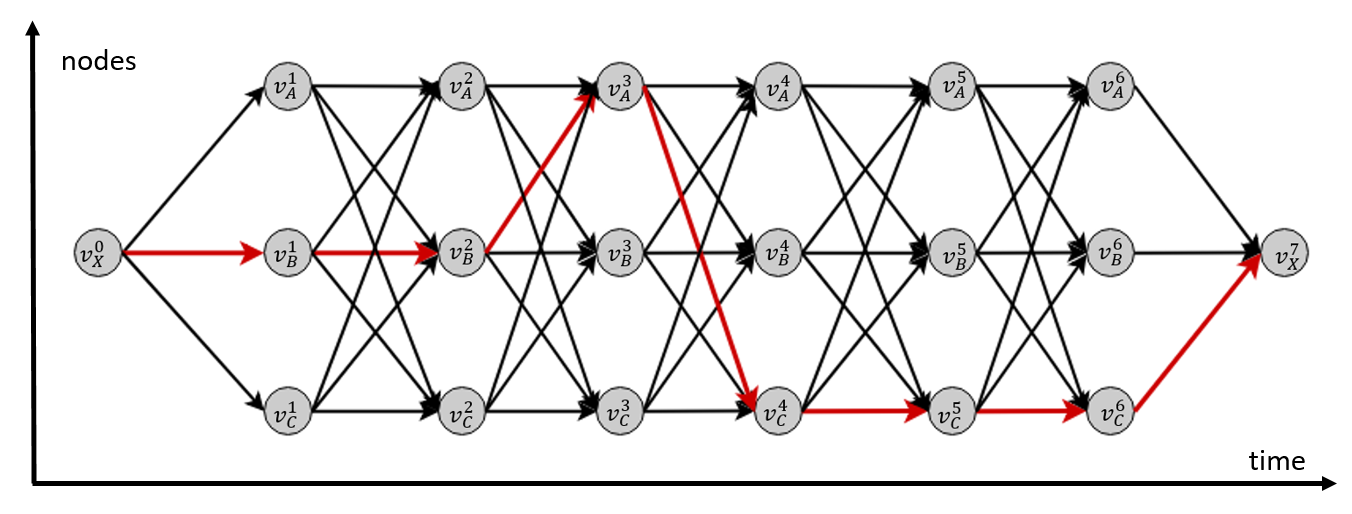
\includegraphics[width=1.0\columnwidth]{./imgs/multipartite_axis.png}
  \caption{Illustration of a Flying Tourist Problem using a multipartite graph. To each node (A,B,C) it is associated a waiting period of respectively (1,2,3) time units. The red arrows represent a possible solution to the problem.}
  \label{fig:multipartite_sol}  
\end{figure}


Despite the apparent complexity of the proposed definition, it can be used to
state very simple flight searches, including one-way and round-trip flights. For
example, the problem of finding a single flight from $A$ to $B$ at date $T$ can
be instantiated as a FTP given by $v_0$ = $A$, $v_{n+1}$ = $B$, $T_{0} = T$, and
$V$ = $D$ = $TW$ = $\{\}$. In its turn, a round-trip flight involving the same
two cities and the same start date, in which the staying period in $B$ is $b$
days, is given by $v_0 = v_{n+1} = A$, $T_{0} = X$, $V = \{B\}$, $D = \{b\}$ and
$TW$ = $\{\}$. Thus, this definition is adequate either for simple and complex
trips, which can be customized according to the user search criteria, by setting
either an extended start dates, or flexible durations.
\section{Relation to the Traveling Salesman}
\label{sec:ftp_tsp}

The Traveling Salesman is the problem of, given a list of cities, finding the best route to visit them all, according to some objective function. In its turn, the Flying Tourist Problem proposed in section \ref{sec:ftp} intends to find the best route, schedule, and set of flights to visit a given list of cities. This section will explore some of these characteristics which distinguish the FTP from the TSP.

It is possible to reduce the Flying Tourist Problem into the Traveling Salesman, a series of reductions, presented below, have to be performed. 

\begin{enumerate}
      \item $v_{n+1} = v_0$;
      \item $T_0 = 0$;
      \item $TW(i) = [0, +\infty[$, $\forall i \in V$;
      \item $D(i) = 1$, $\forall i \in V$;
    \item $c_{ij}^{t} = c_{ij}$, $\forall i, j \in V$, $\forall t$.
\end{enumerate}

Constraint $1)$ operates over the depot, forcing the initial and final node to be the same. While this constraint is not forced on the FTP, because a user might not necessarily want to finish the trip where it was initiated, the TSP considers a single depot. 

Constraint $2)$ is responsible for limiting the start-period to a single time-unit. In a real-world flight search application, this constraint is extremely undesirable, as it reduces the overall quality of the search.

Constraint $3)$ removes the time-windows constrains imposed to each city. This mean that any city might be visited during any time period.

Constraint $4)$ forces each city to be visited during exactly one time-unit. Once again, this constraint is extremely undesirable in a flight search application, since in most cases, users do not want to spend only one night in a destination.

Finally, constraint $5)$ removes the time-dependencies of the cost matrix. It should be noted that the characteristics of commercial flights contradict this constraint.

Applying constrains (1-4) to the proposed Flying Tourist Problem leads to the time-dependent Traveling Salesman Problem, as defined in section \ref{sec:TDTSP_ILP}.

Constraints (1-4) together with (5) reduce the proposed FTP into the asymmetric Traveling Salesman Problem. In order to reduce it to the classical symmetric TSP, it would be necessary to apply an additional constraint which would force the symmetry of the cost matrix.

Given that the Flying Tourist Problem occurs as a generalization of the Traveling salesman, and given that the latter belongs to the class of NP-hard problems \cite{np_completeness}, than so does the former one.




\section{Graph construction}
\label{sec:ftp_graph}



As described in section \ref{sec:ftp}, a Flying Tourist Problem instance is completely described by a structure 
$G =(V_c, A, T_{0}, D, TW)$. Note that the previously referenced structure requires a set of arcs $A$ connecting every pair of nodes belonging to $V_c$. Thus, it is possible to represent this information in a weight matrix, where each of its entries corresponds to a particular arc.

Since the Flying Tourist Problem wishes to address a real-world situation involving commercial flights, upon constructing the weight matrix, it is necessary to take the characteristics of commercial flights into account. For any pair of cities, at any given moment in time, there are several commercial flights which connect these two cities in that particular moment. Given that there is a direct mapping between commercial flights and FTP arcs, than there are multiple arcs for each weight matrix entry. Moreover, a commercial flight connecting two cities does not have a constant price over time. Thus, the value of an arc connecting two cities, varies over time. This means that a weight matrix of a FTP instance is three dimensional, with three variables $i, j, t$, where $i$ is the origin node, $j$ the destination node, and $t$ the moment in time at which the transition occurs.

It is possible to consider a weight matrix in which, for every entry, there are multiple values, corresponding to the different possible arcs for that pair of nodes and time. Consequently, accessing a particular arc requires not only the triplet $(i, j, t)$, but also some information about which particular arc to select. 

Given that the dimensions of a FTP weight matrix are considerable, considering a family of arcs for each weight matrix entry is not recommended, since it would increase the weight size even more. Instead, a pragmatic strategy is followed. Upon constructing a weight matrix for the FTP instance, the objective function is taken into account. This means that, instead of considering that there are multiple arcs for the triplet $(i, j, t)$, it is considered that there is only one: that which has the minimum value according to the objective function. For example, if the objective function intends to minimize the total trip cost, upon constructing the weight matrix, for each family of arcs $(i, j, t)$, only the minimum cost arc would be selected. Using this strategy, for each cost matrix entry, there is only one available arc, and it is the one which minimizes the objective function.

Another important characteristic of commercial flights is that the price of a flight depends on the direction of the traversal. This means that the weight matrix of the FTP is not necessarily symmetric. Moreover, there is also no guarantee that a commercial flight between two cities exist. In fact, there are many cities which do not have a direct flight connection. Fortunately, many commercial flight providers have this into consideration, and try to establish an indirect connection between any two cities, by adding connecting flights. However, this is not always the case, and thus, it is necessary to initialize each entry of the weight matrix to a very high value, in order to discard these non-existent flights from a possible solution.  

To conclude the analysis of the characteristics of the FTP weight matrix, it is worth mentioning that the matrix does not need to be complete, because not every arc is relevant for the construction of a solution. While it is necessary to have every arc connecting two pair of nodes belonging to the set of nodes to be visited, it is not necessary to have every arc connecting the initial and final nodes to the others. In reality, the arcs leaving from and returning to the initial and final node, respectively, are only necessary in particular moments of time. To better understand this, consider figure \ref{fig:arc_families}, which illustrates the necessary arcs to construct a solution to a FTP instance. Every arc of a FTP instance can be classified into three different groups, according to their characteristics: \textit{initial}, \textit{transition} and \textit{final} arcs.

%% ----- use this figure to explain the arc families -----
\begin{figure}[htpb]
  \centering
  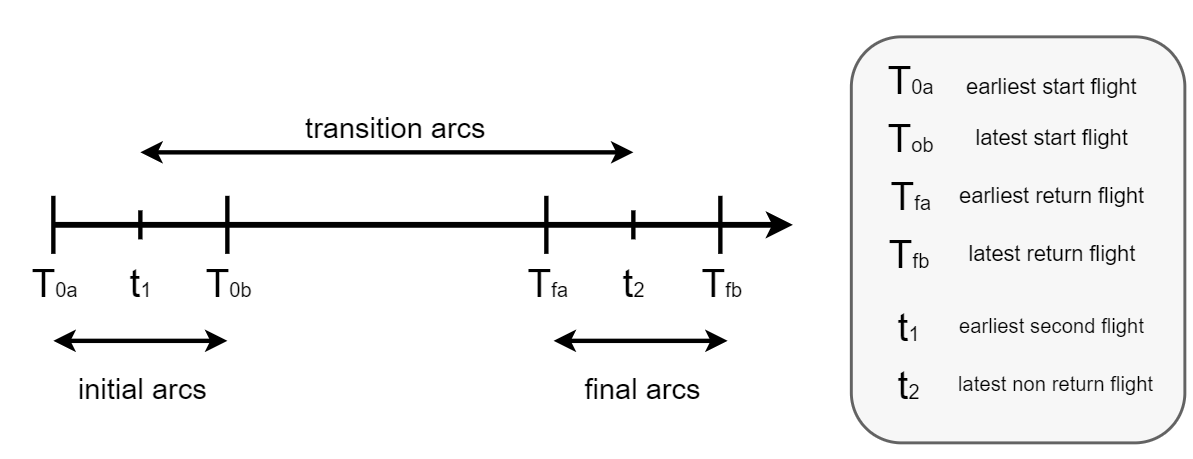
\includegraphics[width=\textwidth]{./Figures/system_design/flights_times.png}
  \caption{Illustration of the distribution in time of the initial, final and transition arcs.}
  \label{fig:arc_families} 
\end{figure}

The \textit{initial} arcs are those which might initiate the trip. Consequently,
they must start at node $v_0$, at $t \in T_0 = [T_{0m}, T_{0M}]$,
connecting $v_0$ to every node in $V$. In its turn, the \textit{final} arcs are those which connect every node in $V$ to
the return node, $v_{n+1}$ at $t$ \in [$T_{fm}$, $T_{fM}$], where $T_{fm}$ =
$T_{0m} + \sum(D)$ and $T_{fM}$ = $T_{0M} + \sum(D)$, and $\sum(D)$
is the total trip duration. There are a total of $k_i = T_{0M} -
T_{0m} + 1$ initial and final arc layers. In the example
depicted in Figure~\ref{fig:multipartite_sol}, there is a single initial and
final layer, since there is only one possible start date.

The \textit{transition} arcs are those which fully connect the $N$ nodes
belonging to $V$. The earliest transition arc occurs at a time no sooner than
$t_1 = T_{0m} + min(D)$, where $min(D)$ corresponds to the lowest value of the
set of durations. Hence, if the trip starts by traversing an initial arc
at time $T_{0m}$, the first transition arc must only be traversed $min(D)$
time-units later. By following a similar approach, the latest transition arc can
occur no latter than $t_2 = T_{0M} + \sum(D) - min(D)$. Thus, there are a total
of $k_2 = t_2-t_1+1$ transition layers, and $k_2*n*(n-1)$ transition arcs.

The union of the initial, transition and final arcs gives the set $A$ of all the
arcs, which may be used to construct a solution to the requested trip. 

\todo{If we can afford an extra page, an analysis of the dimensions involved could be interest. Solution set dimensions, Weight matrix dimensions, memory consumption, relation with instance size, relation with trip duration and start dates}


\section{Optimization methodology}
\label{chap:os}

This section introduces the considered optimization algorithms to produce a solution to a Flying Tourist Problem, as defined in section \ref{sec:ftp}. Given the real-world application under development, and its goals, the devised optimization system should be capable of providing a stream of responses in finite-time. Due to these objectives, the considered optimization strategies are based on heuristic algorithms (subsection \ref{sec:heuristic}) and metaheuristics algorithms (subsection \ref{sec:meta}), as the characteristics of these algorithms fit the goals of the system.



\subsection{Heuristic algorithms}
\label{sec:heuristic}

\input{./Chapters/3.PF/os/heuristic/random.tex}
\input{./Chapters/3.PF/os/heuristic/nn.tex}
%% \input{./Chapters/4.OS/heuristic/two_opt.tex}


\subsection{Metaheuristic algorithms}
\label{sec:meta}

\input{./Chapters/3.PF/os/meta/aco.tex}
\input{./Chapters/3.PF/os/meta/sa.tex}


\section{Summary}
\label{sec:summary_pf}

This chapter enabled the definition of a problem (FTP) which is adequate for the characterization of both simple and complex trips. The instantiation of this problem requires a weight matrix where each of its entries corresponds to a single flight. This problem was shown to be a generalization of the TSP and thus, it belongs to the class of NP-hard problems. Due to its computational complexity, the methodologies proposed to solve the problem rely on heuristic and metaheuristic optimization algorithms.
\cleardoublepage

% %Chapter 4
%\acresetall
%\fancychapter{Optimization System}
\label{sec:os}

This chapter introduces the considered optimization algorithms to produce a solution to a Flying Tourist Problem, as defined in section \ref{sec:ftp}. 
Given the real-world application under development, and its goals, the devised optimization system should be capable of providing a stream of responses in finite-time. Due to these objectives, the considered optimization strategies are based on heuristic algorithms (section \ref{sec:heuristic}) and meta heuristics algorithms (section \ref{sec:meta}), as the characteristics of these algorithms fit the goals of the system.




\section{Heuristic algorithms}
\label{sec:heuristic}

\subsection{Pseudo-random construction procedure}
\label{sec:pseudo_random}

The method introduced in this subsection is not an optimization algorithm, but rather a solution construction procedure for the Flying Tourist Problem. This procedure is relevant for two reasons. First, it can be used to construct a solution to a request in a very fast manner. Of course, the quality of this solution may be extremely poor, but it is very useful as an initial and fast response to a user request. 
Furthermore, this construction procedure is also relevant, because some optimization algorithms, like the Simulated Annealing discussed in section \ref{sec:sa}, require an initial valid and complete solution.

The method introduced below will be hereinafter called pseudo-random construction procedure, and requires an instance of the Flying Tourist Problem $G=(Vc,A,T_0,D,TW)$ where there are no restrictions regarding the time-windows, that is $TW(i) = [0, +\infty[$, $\forall i \in V$. Note that this procedure is both adequate for single and round flights, as well as FTP instances with many nodes to visit. The procedure can be summarized as follows:

\begin{enumerate}
\itemsep0em 
    \item set an initial empty solution: $s=()$;
    \item set the current time to one of the possible start dates: $t \in T_0=[T_{0i}, T_{0f}]$;
    \item set the current node to the start node: $v_c = v_0$;
    \item if the set of nodes to visit, $V$, is empty, go to step 11); else, continue to step 5)
    \item select the next node by choosing a random node from the set of nodes to visit: $v_i \in V$;
    \item remove the selected node from the set of nodes to visit: $V=V\backslash\{v_i\}$;
    \item extend the solution with the arc: $a_{v_c, v_i}^t$;
    \item increment the time according to the duration of visit of the selected node: $t=t+d(v_i)$;
    \item update the current node: $v_c=v_i$;
    \item go to step 4);
    \item extend the solution with the final arc $a_{v_c, v_{n+1}}^t$;
\end{enumerate}
\subsection{Nearest neighbour}
\label{sec:nn}

The nearest neighbour is a solution construction procedure, which starts with an initial empty solution, and at each step of the algorithm updates the current solution be extending it with a solution component, an arc. Thus, this construction procedure is very similar to the one described in subsection \ref{sec:pseudo_random}. However, while the previous construction procedure selects the next node to visit in a pseudo-random way, the nearest neighbour heuristic takes a different approach, selecting the next node according to some particular objective.

During the development of this work, two different nearest neighbour heuristic were used. The first takes into account only the distance between nodes, visiting always the closest node relative to the current one. This is exactly the nearest neighbour procedure applied to the Traveling Salesman Problem. The second approach, instead of considering the distance between nodes, considers the objective function. That is, if the objective is to minimize the total cost, than this heuristic will always select the node according to the minimum cost arc. In its turn, if the objective is to minimize the flight time, or any other criteria, than it is this criteria that is used upon selecting a node to visit, always choosing the node which minimizes the increase in the current objective function. 

In order to distinguish the two nearest neighbour heuristic, we will denote them as \textit{dNN} and \textit{rNN}, that is, \textit{distance} nearest neighbour and  \textit{refined} nearest neighbour, respectively. Note that the first takes into account only the distance between nodes, and not directly the objective function, while the latter only takes into account the objective function, and disregards completely the distance between nodes.

The nearest neighbour construction procedure can be adapted from the previously introduced pseudo-random construction procedure by replacing only the construction step number 5). Thus, the distance nearest neighbour considers:

\begin{itemize}
    \item select the next node by choosing the one closest to the current node: \newline
    $v_i$ $\in$ $V$: $d(v_c, v_i)$ $\leq$ $d(v_c, v_j)$,
    $\forall$ $v_j$ $\in$ $V$ $\backslash$ $\{v_i\}$   
\end{itemize}

while the refined nearest neighbour considers:


\begin{itemize}
    \item select the next node by choosing the one which increases the objective function the least: \newline
    $v_i$ $\in$ $V$: $f(v_c, v_i)$ $\leq$ $f(v_c, v_j)$,
    $\forall$ $v_j$ $\in$ $V$ $\backslash$ $\{v_i\}$   
\end{itemize}

It is worth nothing that applying the distance and the refined nearest neighbour heuristics require different levels of information. On one hand, the distance nearest neighbour requires only the distances between each pair of cities. On the other hand, the refined nearest neighbour requires a complete weight matrix regarding the objective function.




%% \subsection{2-opt}
\label{sec:two_opt}

The 2-opt algorithm is a local search procedure developed for the resolution of the Traveling Salesman Problem \cite{two_opt_croes}. 



\section{Metaheuristic algorithms}
\label{sec:meta}

\subsection{Ant Colony Optimization}
\label{sec:aco}

The considered Ant Colony Optimization (ACO) algorithm receives, as input, a weight matrix with the information regarding all solution components of the problem. It must also receive other relevant parameters for the solution construction process, as the initial and final node and the set of waiting periods $D$. 

\todo{Add reference for the $\tau_0$}
The initialization of the ACO metaheuristic requires the construction of an initial pheromone matrix. Each entry of this matrix is set to an initial pheromone value, according to Eq.~\ref{eq:tau_zero}, where $n$ is the number of nodes and $C^{nn}$ is the cost of the nearest neighbor heuristic. 
\begin{equation}
\label{eq:tau_zero}
  \tau_{ij}^{t} = \tau_{0} = \frac{1}{nC^{nn}}
\end{equation}

The initialization of the metaheuristic also requires the definition of a variety of algorithm-specific parameters, such as the number of ants $m$, the pheromone evaporation rate $\rho$, the heuristic relative influence $\beta$, the pheromone relative influence $\alpha$, and the exploration rate $Q_0$. 

After the initialization, and until the termination condition is met, the algorithm enters an iterative cycle, where every ant belonging to the colony constructs a solution to the problem. This is followed by a pheromone update phase, to reflect the colony search experience. A new iteration may only start after all ants have finished the solution construction process and the pheromone matrix has been updated.

%The construction process that is undertaken by each ant is as follows. First, the current time is set to a value belonging to the allowable trip start dates, $t \in T_0$, and the current node is set to the start node $v_0$. Each ant enters an iterative cycle until all nodes belonging to $V$ are visited. At every step of this cycle, an ant chooses a solution component by either \textit{exploiting} or \textit{exploring} the search space. The decision of exploiting or exploring depends on the algorithm parameter $Q_0$ and on a pseudo-random value $q$, calculated at run time. The selection of the solution component $j$, which identifies the next city to be visited, is given by Eq.~\ref{eq:selection_rule}. After the selection of each solution component, it is necessary to update the time, incrementing it by the duration relative to the selected city.

The construction process undertaken by each ant is as follows. First, the current time is set to a value belonging to the allowable trip start dates, $t \in T_0$, and the current node is set to the start node $v_0$. Each ant enters an iterative cycle until all nodes belonging to the set of nodes to visit, $V$, are visited exactly once. At every step of this cycle, an ant chooses one of the remaining valid solution components. The selection of a particular solution components depends on multiple factors, as the solution component cost and its pheromone value. After the selection of each solution component, it is necessary to update the current time, by incrementing it  according to the duration of the selected city. By following this iterative construction process, a valid but incomplete solution is found. To complete this solution, it is necessary to add an extra solution component, which closes the route by adding the return node, $v_{n+1}$.

In the construction process described above, each ant selects the next solution component by either \textit{exploiting} or \textit{exploring} the search space. That is, exploitation is the process of selecting the next solution component mostly based on the previous ants' search experience, while exploration intends to diversify the traversed search space. The decision of exploiting or exploring depends on the algorithm parameter $Q_0$ and on a pseudo-random value $q$, calculated at run-time. The selection of the solution component $j$, which identifies the next city to be visited, is given by Eq.~\ref{eq:selection_rule}. 

\begin{equation}
  \label{eq:selection_rule}
  j =  \left \{
    \begin{aligned}
      & exploitation \ (\text{Eq.} \ \ref{eq:exploitation}) , && \text{if}\ q \leq Q_0 \\
      & exploration \ (\text{Eq.} \ \ref{eq:exploration}), && \text{otherwise}
    \end{aligned} \right. 
\end{equation}

The \textit{exploitation} of the search space utilizes the \textit{pseudorandom proportional} rule, defined by Eq.~\ref{eq:exploitation}, which determines the next solution component of the ants' solution. The $J_k(i,t)$ term represents the set of solution components that might be selected to form a valid solution component by an ant in its current \textit{state}, where the state refers to the current ant position of the trip it has constructed so far.
\begin{equation}
  \label{eq:exploitation}
    arg max_{j \in J_k(i,t)} {[\tau(i,j,t)][\eta(i,j,t)]^\beta}
\end{equation}

On the other hand, the \textit{exploration} is given by Eq.~\ref{eq:exploration}, with $p_a(i,j,t)$ representing the probability of ant $a$ (which is currently at node $i$ at time $t$) selects $j$ as the next node to visit.
In the presented equations, $\eta$ is the inverse of the weight matrix value.
\begin{equation}
\label{eq:exploration}
  p_a(i,j,t) =  \left \{
    \begin{aligned}
      & \frac{[\tau(i,j,t)][\eta(i,j,t)]^\beta}{\sum_{u \in J_k(i,t)}[\tau(i,u,t)][\eta(i,u,t)]^\beta}, && \text{if}\ j \in J_k(i,t) \\
      &0, && \text{otherwise}
    \end{aligned} \right. 
\end{equation}

%By following an iterative construction procedure, a valid but incomplete solution is found. To complete this solution, it is necessary to add an extra solution component, which closes the route by adding the return node, $v_{n+1}$.

After each ant finishes its iterative solution construction process, the ACO metaheuristic enters into its pheromone update step. Depending on the chosen ACO algorithm, the pheromone update may vary. This work follows the Ant Colony System (ACS) strategy, whose pheromone update requires both a deposit and an evaporation step. Unlike many other ACO algorithms, the pheromone update applies only to the arcs belonging to the best solution found so far, $S_{bs}$. This results in the update of the pheromone values by means of Eq.~\ref{eq:pheromone_update}, where $(\Delta\tau_{ij}^{t})^{bs}$ is given by $1/C^{bs}$, where $C^{bs}$ represents the objective function value of the best solution.
\begin{equation}
\label{eq:pheromone_update}
    \tau_{ij}^{t} = (1-\rho)\tau_{ij}^{t} + \rho (\Delta \tau_{ij}^{t})^{bs}
\end{equation}

It is common (and often recommended) to combine ACO algorithms with local search heuristics, also denoted \textit{daemon actions}, that try to improve the quality of the constructed solutions, after each of the ants' iterative cycle. However, this was not applied to the proposed optimization, due to the nonexistence of adequate local search procedures for the time-dependent TSP. In fact, even the $k$-opt exchange procedures, widely used in the classical TSP as local search, are not efficient for the time-dependent TSP because it requires, at each step, the computation of the entire trip cost, as opposed to just the cost difference regarding the $k$ arcs, as in the symmetric TSP.






\subsection{Simulated Annealing}
\label{sec:sa}

The developed Simulated Annealing algorithm receives, as input, a weight matrix with the information of the solution components of the problem. It must also receive other relevant parameters for the solution construction process, as the initial and final node and the set of waiting periods $D$. This specific information about the instance under optimization is crucial, as it enables the validation of a solution and the calculation of the objective function value.

The general procedure of the Simulated Annealing metaheuristic is as follows. Given an initial solution ($x$), at each step of the inner cycle (also called Markov chain), a new candidate solution ($y$) is constructed based on a neighbourhood function, which is usually problem specific. Depending on the quality of the new solution, and the current temperature of the algorithm, this solution may or may not be accepted. This process of constructing and conditionally accepting a new solution occurs a fixed number of times per outer cycle - this number if referred to as the Markov chain length. Having completed one Markov chain, the temperature of the state is decreased, according to a predefined cooling schedule.

Given the above described procedure, the Simulated Annealing is a metaheuristic which requires:
\begin{enumerate}
    \item an initial solution;
    \item a neighbourhood function - used to construct candidate solutions; 
    \item an acceptance criteria - used to conditionally accept the candidate solutions;
    \item a cooling schedule - to decreasing the temperature of the state;
\end{enumerate}


The Simulated Annealing is a local search metaheuristic, which conditionally accepts uphill moves, allowing it to escape from local minimum. As any local search algorithm, it requires an initial solution.  It is possible to construct this initial solution by applying the pseudo-random construction procedure (section \ref{sec:pseudo_random}), or using the nearest neighbour (section \ref{sec:nn}). In general, the quality of the initial solution does not affect the quality of the best solution found by the algorithm.

The neighbourhood function selected for the generation of new candidate solutions is the 2-opt swap procedure. Hence, at each iteration step of the Markov chain, it selects two random nodes and swaps the corresponding path. It is also necessary to take into account both the initial and final nodes in order to produce a valid solution. Since this swapping procedure may change the dates at which each node is visited, which consequently changes the solution arcs, it is necessary to adjust the flight dates and calculate the objective function value of the candidate solution.

%The acceptance criteria used by the developed Simulated Annealing algorithms is the Metropolis acceptance criteria \cite{metropolis}, presented in Eq.~\ref{eq:metropolis}. This criterion dictates that: (i) if a candidate solution $y$ is \textit{better} than the current solution $x$, it is always accepted; (ii) if the solution is worse, it may, or may not be accepted. The probability by which a worse solution is accepted depends upon: a) the difference in the objective function values $\Delta_f$ of the two solutions; b) the current temperature of the system. As $\Delta_f$ increases, and as the temperature decreases, the probability of accepting a worse solution is reduced. With such an approach, the Metropolis acceptance criteria allows up-hill moves, which enable the algorithm to escape from local minimum. Notwithstanding, as the temperature reaches very low values, the algorithm becomes increasingly greedy.

The acceptance criteria is a function which determines the probability of accepting a candidate solution, which is compared to a pseudo-random value generated at run-time, and dictates if a candidate solution is, or is not, accepted. The developed Simulated Annealing algorithms uses the Metropolis acceptance criteria \cite{metropolis}: 
\begin{enumerate}
    \item if a candidate solution $y$ is \textit{better} than the current solution $x$, it is always accepted;
    \item if a candidate solution is worse, it may, or may not be accepted;
    
\end{enumerate}

The probability by which a worse solution is accepted depends upon the difference in the objective function values $\Delta_f$ of the two solutions and the current temperature of the system (Eq.~\ref{eq:metropolis}). As $\Delta_f$ increases, and as the temperature decreases, the probability of accepting a worse solution is reduced. With such an approach, the Metropolis acceptance criteria allows up-hill moves, which enable the algorithm to escape from local minimum. Notwithstanding, as the temperature reaches very low values, the algorithm becomes increasingly greedy.

% METROPOLIS ACCEPTANCE RULE
\begin{equation}
\label{eq:metropolis}
  p =  \left \{
  \begin{aligned}
    & 1, && \text{if}\ f(y) \leq f(x),\\
    & e^{-\frac{\Delta_f}{t}},&& \text{otherwise}
  \end{aligned} \right. 
\end{equation}

% The developed SA optimization uses a geometric cooling schedule. It starts with an initial temperature $t_0$, and at each outer iteration, the temperature is decreased to $t_{k+1} = \lambda * t_{k}$, where $k$ is the iteration counter of the outer loop and $\lambda$ is the cooling parameter. 

The developed SA optimization uses a geometric cooling schedule. It starts with an initial temperature $t_0$, and at each outer iteration, the temperature is decreased, using equation \ref{eq:cooling}, where $k$ is the iteration counter of the outer loop and $\lambda$ is the cooling parameter. 

\begin{equation}
    \label{eq:cooling}
     t_{k+1} = \lambda * t_{k}
\end{equation}

The cooling schedule parameters $t_0$, $t_f$ and $\lambda$ must be calculated beforehand based on the probability of accepting a worse solution during the first iteration ($p_0$) and during the last iteration ($p_f$), and on the total number of outer iterations ($k$). The defined algorithm establishes $p_0$ as $0.98$ and $p_f$ as a positive value close to zero. The total number of iterations is set according to the time available for the optimization process, and the length of the Markov chain ($M$) is set to the number of nodes $m$.

% In this work, the implemented Simulated Annealing algorithm uses a geometric cooling schedule, with parameter $\lambda$, and a simple 2-opt technique for the neighborhood function. The initial temperature $t_0$, is set in such a way that the initial probability $p_0$ of accepting a worse solution is 0.98. In its turn, the final temperature $t_f$ is such that the probability $p_f$ decreases to $10^{-300}$. By setting $p_0$ and $p_f$, and given that a geometric cooling schedule implies that $t_{k+1} = \lambda * t_{k}$, where $k$ is the iteration counter, it is possible to use the Metropolis acceptance criteria to define the initial and final temperatures. Note that this requires that the algorithm performs a fixed number of iterations, defines apriori. 

To calculate the value of $t_0$ and $t_f$, the algorithm starts by generating some candidate solutions using the neighborhood function and the current solution $x$ (\cite{SA_methods}). These candidate solutions are used to calculate the average absolute difference in the objective function $\Delta_{avg}$. This allows the calculation of the  $t_0$ value according to Eq.~\ref{eq:t_zero}, based on the Metropolis criteria. The final temperature $t_f$ is given by $t_f = \lambda^{k}t_0$. This allows the calculation of $\lambda$ with Eq.~\ref{eq:lambda}. Given $t_0$, $t_f$ and $\lambda$, the geometric cooling schedule is completely defined.

\begin{equation}
\label{eq:t_zero}
    t_0 = \frac{-\Delta_{avg}}{ln(p_0)}
\end{equation}

\begin{equation}
\label{eq:lambda}
    \lambda = \bigg( \frac{-\Delta_{avg}}{ln(p_f)t_0} \bigg)^{1/k}
\end{equation}

% Having a complete cooling schedule and neighborhood function, the Simulated Annealing has almost all parameters required. The only thing missing is information about the length of the inner cycle, the Markov chain. That is, the metaheuristic implements two cycle, where the most inner cycle, the Markov chain, is responsible for generating new solutions, and the outer cycle is responsible for controlling the temperature. The number of the iterations of the inner cycle is given by $m$, and of the outer cycle by $k$. It is common to specify both values apriori, and to define $m$ as a function of the length of the neighborhood structure. In this work, $m$ is set to be equal to the number of nodes.

%Finally, it is necessary to define the length of the Markov chain. Following the suggestions of the literature, the length of the Markov chain, $m$ is set to be equal to the number of nodes. \todo{Vou tentar melhorar este} 


















%\cleardoublepage
%
%Chapter 5
\fancychapter{System Design}
\label{chap:SD}

One of the objectives addressed by this work is the development of a flight search application to solve unconstrained multi-city flight requests. Chapter \ref{chap:pf} presented a formal definition of the problem, and chapter \ref{chap:os} covered some possible ways to solve it. In its turn, this chapter presents an overview of the architecture (section \ref{sec:system_architecture}), structure and design choices (sections \ref{sec:csa_design} and \ref{sec:ssa_design}) of the proposed web application.
\section{System Architecture}
\label{sec:system_architecture}

The aimed web application should allow users to search for the best schedule, route and set of flights, for both one-way and round-trip flights, as well as unconstrained multi-city trips. During the formal definition of the problem, in section \ref{sec:ftp}, it was shown that these problems can be converted into a FTP instance, which is a generalization of the TSP. Because of this, as the number of cities increases, the problem becomes increasingly more difficult to solve. In order to cope with this, each user defined request is solved using the optimization algorithms previously presented in chapter \ref{chap:os}.

The proposed system is structured into two separate applications: the Client Side (CSA) and the Server Side applications (SSA). The client side application is designed to solely interact with the user, redirecting  requests to the server side application, whose goal is to solve these requests. Thus, there is a complete separation of concerns between both applications: the CSA serves only as an input/output port, and the application logic and intelligence is handed by the SSA. The communication between both application relies on the Hypertext Transfer Protocol (HTTP) and on Asynchronous JavaScript and XML (AJAX). This means that the CSA may request data from the SSA using a simple HTTP protocol, and that this communication is asynchronous, allowing the user to continue to interact with the application, even while the response is being prepared. The structure of the proposed application, and the data-flow associated to the resolution of a user defined request are presented in figure \ref{fig:sa_design}.

\begin{figure}[htpb]
  \centering
  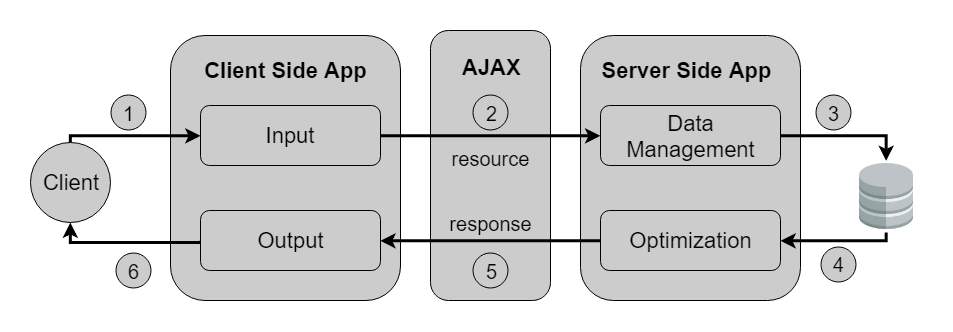
\includegraphics[width=\textwidth]{./Figures/system_design/system_architecture_design.png}
	\caption{Structure and data flow of the proposed application.}
  \label{fig:sa_design}  
\end{figure}


\section{Client Side Application}
\label{sec:csa_design}

The Client Side Application (CSA) is a web application designed to interact with the user, allowing the construction of flight requests and the presentation of meaningful solutions. These requests are not processed directly by the CSA, as it would consume too much resources (CPU and RAM) of the users device, and are, instead, redirected to the SSA to be solved. Thus, the CSA intends to be only an input/output port between the user and the SSA. 

Each user defined request is constructed in such a way that it can be used to instantiate a Flying Tourist Problem, as defined in section \ref{sec:ftp}. Each Flying Tourist Problem request is a specific resource, uniquely identified by a particular Uniform Resource Identifier (URI). This will be further detailed in section \ref{sec:api_protocol}. Each of these resources are used to request a solution to the request from the the server side application. Following this convention, the user interface must enable the collection of:

\begin{itemize}
  \item the start city and return city, $v_{0}$ and $v_{n+1}$, respectively;
  \item a list of cities to be visited $V$, and the durations $D$ associated to each;
  \item the start dates $T_{0}$ associated to the trip;
\end{itemize}

Upon receiving a solution to a user request, the User Interface must be updated, displaying the relevant information of these solutions. Each solution to a request is an object which contains at least one set of flights that satisfy the user defined itinerary. However, a response to a request should 
contain several valid solutions, so that the user might choose the most adequate to his needs.
Each solution is composed of one or several flights, and each of the presented flights should contain, at least, the following information:

\begin{itemize}
  \item the flight cost;
  \item the flight duration;
  \item the date, departure and arrival time;
  \item the number of layover flights;
\end{itemize}

Having a clear idea of the objectives and structure of the Client Side application, it is possible to discuss its actual design. The User Interface can be separated into two independent views: the \textit{Request} and the \textit{Response} view. These views enable the construction of user requests, and the visualization of the constructed response,  respectively. It would also be useful to define and implement a third view: a \textit{Map} view. While the request and response views are essential to the overall function of the application, the map view is not. However, a map capable of displaying the routes of the selected flights, as well as other relevant information, would certainly contribute to a better and more complete user experience.

A web application can be accessed by multiple devices, as phones, tablets and computers, and each of these devices has different screen dimensions. Because of this, the proposed web application should be \textit{responsive}. That is, the design and dimensions of the user interface should be adequate and responsive to the size of the device rendering it.

With this in mind, the proposed User Interface should follow the design illustrated in figure \ref{fig:UI_design}. Notice that there are a total of three views: the response and request views, which are essential, and thus are always present; and the map view, which is not, and thus can be discarded on some smaller devices.

\begin{figure}[htpb]
  \centering
  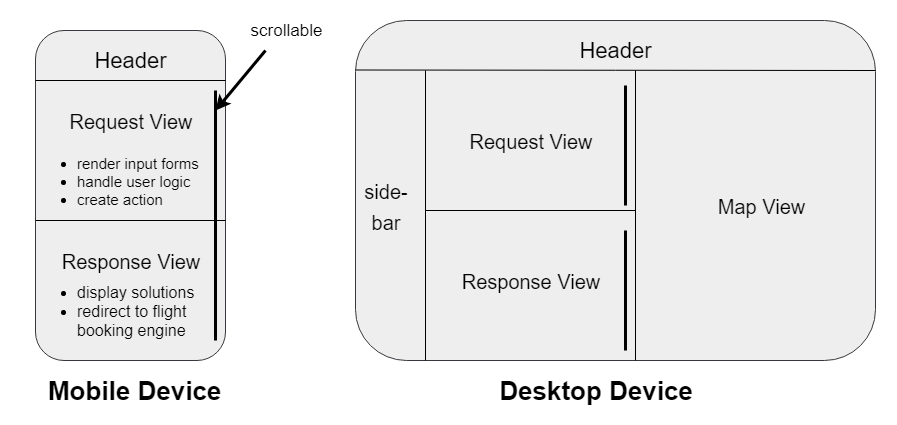
\includegraphics[width=\textwidth]{./Figures/system_design/UI_design.png}
  \caption{Proposed response User Interface for small/medium and large devices. 
  There are 2 essential views and one optional view.}
  \label{fig:UI_design}
\end{figure}

\section{Server Side Application}
\label{sec:ssa_design}

The SSA is responsible for producing a solution to a user defined FTP instance. To do so, the SSA shall be implemented as an Application Programming Interface (API), listening for requests to particular resources, which uniquely identify these FTP instances. Each received request corresponds to a shallow FTP instance, that is, a problem in which the cities are specified, but the flights are not. To overcome this problem, and collect the relevant flight data, the SSA will rely on a \ac{DMS}, discussed in section \ref{sec:dms_design}. Having a complete FTP instance, the SSA will use the Optimization system discussed in section \ref{sec:os_design} to construct a solution to these user requests.




\subsection{Data Management System}
\label{sec:dms_design}
Upon receiving a user defined request, the set of nodes, as already well as the start time and durations, are well defined. On the other hand, the set of arcs which connects these nodes are not. For example, a user request may correspond to a single flight from $A$ to $B$, at time $t$, and, upon receiving this request, there is no available information regarding the possible flights (arcs) between these two cities. In fact, that is exactly what the user is searching for. Thus, the goal of the Data Management System is to collect the necessary information to construct the list of arcs associated to a user request.

%In order to access real flight data, a publicly available flight data API shall be used. This is the simplest, fastest and most efficient way to request flight data. There are several possible choices upon selecting a flight API. As a consequence, the available API's shall be classified as \textit{free}, \textit{limited} and \textit{enterprise}. A free API is one which does not charge or limit the available queries. On the other hand, a limited API is one which sets an upper bound on the number of daily available queries, and charges a fee after this limit. In its turn, an enterprise API is available  only for commercial solutions, and it may not be used in a research context. During the development of this work, only free API's were considered. 

The communication with a flight API utilizes a simple HTTP protocol, and every request is identified according to an Uniform Resource Identifier, whose syntax is defined by the API provider. A response to a request usually consists in a data tree, by using a structured data format, such as \ac{JSON}. Every response includes a list of possible flights, and each flight has a vast number of attributes, as the cost, flight duration, departure time, and so on.

Although there are several publicly available flight data API's, the information provided by each of those might be considerably different. Multiple flight search applications were compared in chapter \ref{chap:introduction} from a simple services offer perspective, and the results were presented in tables \ref{tab:single_round_flights} and \ref{tab:multi_flights}. The analysis of this comparison from the corresponding API perspective shows that the flight data presented by each of these API's varies considerably. For example, the cost of a single flight may be up to 44\% higher, according to the API flight data provider. 

Hence, one of the main goals of the proposed web application is to find the best set of flights for a given query, according to some objective function and, in particular, the minimization of the total flight cost. Given that there are considerable differences among flight APIs, ideally, the proposed web application should query multiple APIs.

The role of the Data Management System is of crucial importance for the development of a high quality flight search web application. This is because every user request seeks to find a given set of flights to a satisfy a particular itinerary. Thus, it is of extreme importance to have the most up-to-date flight data for each of the possible flights.  



\subsection{Optimization system}
\label{sec:os_design}
The goal of the Optimization System (OS) is to produce solutions to user defined Flying Tourist Problem instances. Upon defining an itinerary and translating it to a FTP instance, the arcs which connect the nodes are not defined, and thus, no valid solution can be produced. Thus, the OS is heavily dependent on the Data Management system, as it requires relevant flight data to process the requests. 

Depending on the particular request being processed, the time necessary to collect all the necessary flights, or the time necessary to run a computationally heavy optimization algorithm, might be very high. Because of this, the optimization system is distributed into different layers, as illustrated in figure \ref{fig:optimization_system}, which require different amount information regarding the flights, and produce multiple solutions using different heuristics, at different times. The goal of this is to reduce the latency felt by the user, by producing an initial solution as soon as possible, and continue to search for a better one afterwards.

\begin{figure}[htpb]
  \centering
  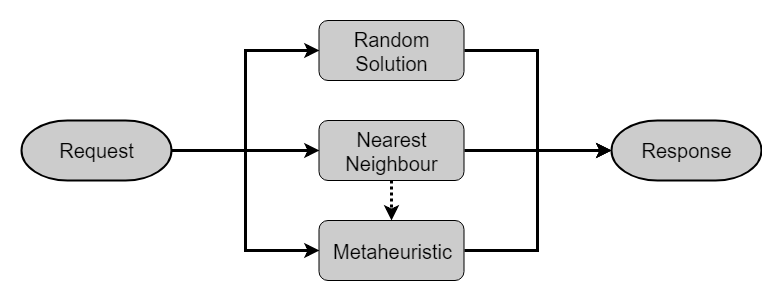
\includegraphics[width=\textwidth]{./Figures/system_design/utility.png}
  \caption{Simplified illustration of the optimization system, which utilizes different algorithms 
  to produce a solution to a user defined request.}
  \label{fig:optimization_system}  
\end{figure}

The first layer of the optimization system implements the random solution construction procedure, proposed in section \ref{sec:pseudo_random}. This procedure enables the construction of a solution in a very fast manner, as it randomly selects one node after another, and only requires information regarding a very limited number of flights. Despite producing a very fast solution, the quality of it is expected to be low.

The second layer of the OS implements the nearest neighbour heuristics proposed in section \ref{sec:nn}. The implementation of this heuristic requires information regarding the entire weight matrix associated to the problem. Because of this, it must run only after constructing the initial solution. It is expected that the solution constructed by this procedure is of higher quality to the initial one.

In its turn, the third layer of the OS implements the meta-heuristic optimization algorithms proposed in section \ref{sec:aco} and \ref{sec:sa}. As occurs with the nearest neighbour heuristic, these optimization algorithms require information regarding the entire weight matrix. Thus, they must also run only after the initial solution construction procedure, but they might run in parallel with the nearest neighbour heuristic. It is expected that the solutions constructed by these meta-heuristics is of much better quality than the initial and the nearest neighbour solutions.



\section{Summary}
\label{sec:summary_sd}

This chapter presented the design and implementation details of the proposed flight search web application. In the first part, covering the sections related to the design process, it was presented the considered architecture for the web application, which separates the user interface from the logic associated to the resolution of FTP requests. It also established a design goal for the user interface, and proposed an architecture for the optimization algorithm, as to reduce the latency that is sensed by the users. During the remaining of the chapter, the implementation details regarding these topics were provided.

\cleardoublepage
%
%Chapter 6
%\fancychapter{System Implementation}
\label{cap:SI}

%By following the design proposed in chapter \ref{chap:SD}, this chapter addresses the implementation details of the developed system. This is achieved by first addressing the proposed system as a whole (section \ref{sec:sa_implementation}), followed by an overview of its two main components: the CSA (section \ref{sec:csa_implementation}) and SSA (section \ref{sec:ssa_implementation}). 
\section{System Architecture}

By following the architecture proposed in section \ref{sec:system_architecture} and illustrated in figure \ref{fig:sa_design}, the developed system consists of two web applications: the CSA and SSA. The CSA is the application responsible for rendering the User Interface, allowing the definition of user requests, which are processed by the SSA. Thus, although these two applications run separately, the CSA is dependent upon the SSA. 

%The developed applications are divided into two distinct groups: the Client Side Application (CSA), or the User Interface, and the Server Side Application , or the flight data/optimization API. Both applications run independently from one another, although the CSA is dependent of the API, and must communicate with it as to obtain solutions to the user requests. Figure \ref{fig:system_architecture} introduces the architecture of the system, as well as the technologies on which the system relies, which will be addressed in the rest of this section. 


The developed applications are hosted on \textit{Heroku}, a cloud platform which, upon request, creates two separate runtime environments, one for each application. Each application requires a server to listen to requests and serve content. In particular, the CSA and SSA run on \textit{node.js} and \textit{django} servers, respectively (see figure \ref{fig:sa_structure}. Furthermore, since the User Interface will render a map, the CSA requires access to the Google Maps API. To enable the implementation of a modern web application, the CSA also uses several other frameworks, in particular, React and Redux. In its turn, the SSA requires access to real flight data and thus, will interact with Kiwi's flight data API. The described application structured is illustrated in figure \ref{fig:sa_structure}, and the developed applications are denoted by \textit{Bfly App} and \textit{Bfly API}, for the CSA and SSA, respectively. The previously mentioned underlying technologies will be discussed with further detail in the following subsection.  


\todo{Edit image. Try to reduce size. Change "cloud platform" to "host". Replace bootstrap to Google modular design}

\begin{figure}[htpb]
  \centering
  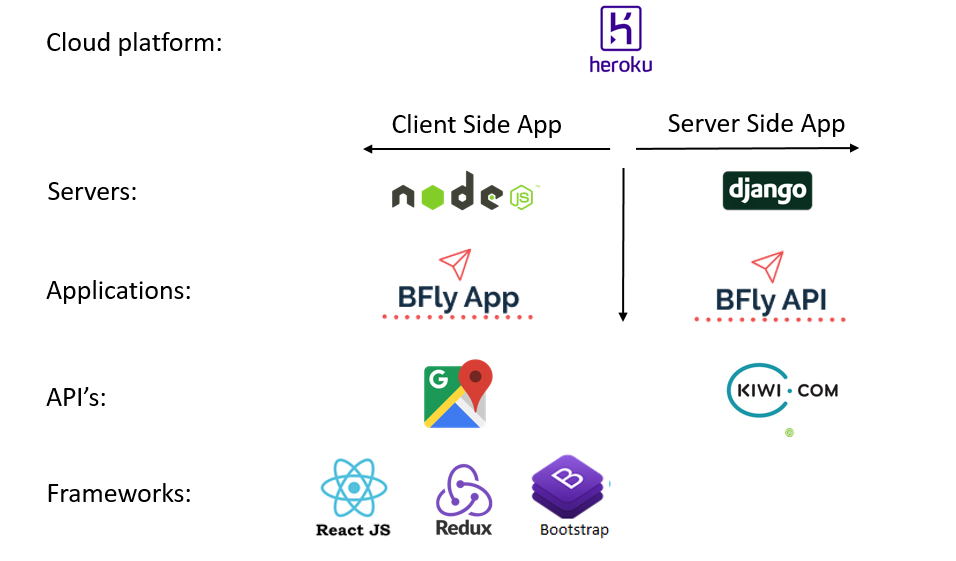
\includegraphics[width=.7\textwidth]{./Figures/system_implementation/system_architecture_implementation.png}
  \caption{Techonology stack used by the developed application.}
  \label{fig:sa_structure}  
\end{figure}


%The developed applications run on \textit{Heroku}, a Cloud Platform as a service, which, upon request, creates two separate servers, one for each application. The Client Side Application runs a \textit{Node.Js} server, which creates a bundle file, that is served to the user, and contains all the necessary information to render the UI, handle the user input logic, and interact with the API. In its turn, the API runs on \textit{Django}, which interacts with the webserver to read the user request, and may execute particular instructions according to the selected route.

\subsection{Underlying technologies}

\subsection{Heroku}
\input{./Chapters/6.SI/SA/tecs/heroku.tex}

\subsection{Node.js}
\input{./Chapters/6.SI/SA/tecs/node.tex}

\subsection{Django}
\input{./Chapters/6.SI/SA/tecs/django.tex}

\subsection{React and Redux}
\input{./Chapters/6.SI/SA/tecs/rr.tex}

% \subsubsection{Google Maps}
% \input{4.SI/SA/tecs/gmaps.tex} 
\section{Client Side Application}
\label{sec:csa_implementation}


The Client Side Application is implemented as a web application to interact with a user and allow the resolution of complex flight requests. The CSA is constructed as a single page application, and is hosted using \textit{heroku}, being publicly available \footnote{The developed CSA has the following URL: \url{https://desolate-castle-31305.herokuapp.com/}}.

The CSA, built using react and redux, evolves around a concept called \textit{state}. The state of the application is stored in the \textit{redux store}, and it contains the relevant information associated to the application at each instance. In the developed application, the state tree is  divided into \textit{requests} and \textit{responses}. Requests are associated to the user input, while responses come from the SSA. The state cycle of the developed application is illustrated in figure \ref{fig:app_state_cycle}.

\begin{figure}[htpb]
  \centering
  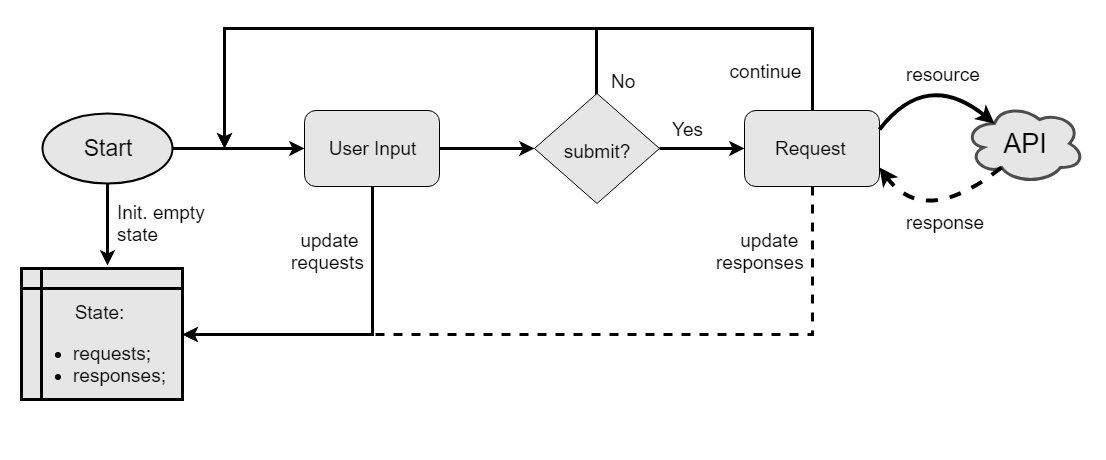
\includegraphics[width=\textwidth]{./Figures/system_implementation/state_flow.png}
  \caption{Block diagram of the state cycle of the Client Side Application.}
  \label{fig:app_state_cycle}  
\end{figure}

To each branch of the state (request and responses) it is associated with a \textit{container} (or a view). Containers are top level components, which access the state directly, and call specific components, often using parts of the state as input (props) for them. Thus, the developed application has two main views, as it was proposed in section \ref{sec:csa_design}. There is also a third container, for the map, although it does not have a state branch for itself, but instead derives the necessary information from the the other two. 

The complete architecture of the implemented react/redux application, including some of the concepts previously discussed, is illustrated in figure \ref{fig:react_redux_app}. This figure illustrates the top down hierarchy, with a single component in the top of the hierarchy (denoted \textit{app.js}), which instantiates the redux store, and renders the complete application, by invoking the containers which are connected to the relevant presentational components. This figure also illustrates the interaction with the store and with third-party API's. 

%Finally, it is important to note that a browser can only render HTML, and the entirety of the application is built using JavaScript. Thus, it is necessary to inject the created JavaScript with all the business and presentation logic, into the HTML file served  to the user. This is usually done by using a package compiler called \textit{Webpack}.

During the remaining of this section, it will be shown how to collect user input (subsection \ref{sec:user_input}) and how to communicate with the SSA  (subsection \ref{sec:api_communication}). Finally, subsection \ref{sec:user_interface_ready} illustrates the developed web application, by presenting some actual screen-shots of it.

\begin{figure}[htpb]
  \centering
  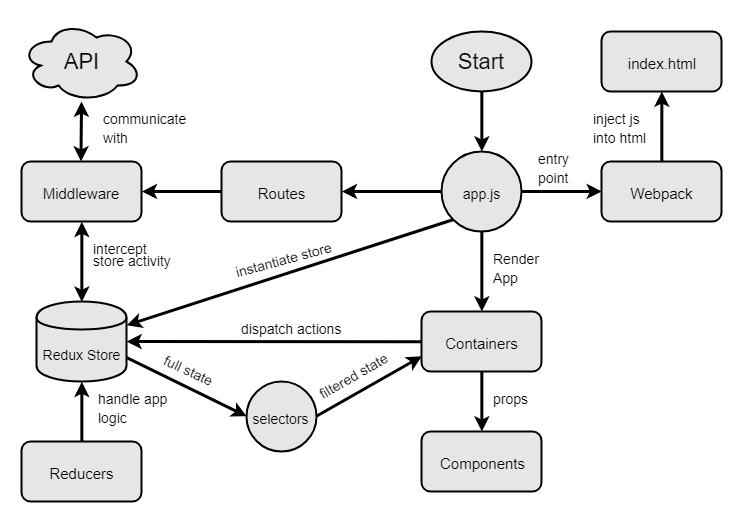
\includegraphics[width=.8\textwidth]{./Figures/system_implementation/react_redux_app.png}
  \caption{Building blocks of an application built using React And Redux.}
  \label{fig:react_redux_app}  
\end{figure}




\subsection{User Input}
\label{sec:user_input}
There are three types of requests that will be processed by the application: single flight, round trip and multi-city trip. A user must initially select the desired type of search, and follow this with the completion of a series of forms that collect the relevant input. 

Every request requires at least an origin and a destination, as well as a start date. There are other search attributes which might be relevant, according to the selected trip type, as the duration associated to each city that will be visited. A complete list of the input that may be collected from the user is presented in table \ref{table:input_action_reducer} (left column). 


\begin{table}[htpb]
  \centering
  \caption{Parallelism between User Input, Actions and Reducers. To each user defined input corresponds an 
  action, declaring the intent of changing the state with some specific data, and a reducer, which actually modifies the state. }
  \setlength{\tabcolsep}{8mm}
  \label{table:input_action_reducer}
  \begin{tabular}{ccc}
  \hline
  \\[-0.75em]
  User input  & Action               & Reducer                    \\ \hline
  \\[-0.75em]
  origin      & actOrigin(origin)    & setOrigin(state, action)   \\
  \\[-0.75em]
  destination & actDest(dest, index) & setDest(state, action)     \\
  \\[-0.75em]
  duration    & actDur(dur, index)   & setDuration(state, action)     \\
  \\[-0.75em]
  start date  & actDate(date, index) & setStartDate(state, action)     \\
  \\[-0.75em]
  submit      & actRequest(request)  & setResponse(state, action) \\ \hline
  \end{tabular}
\end{table}


Then, to every user input it is associated an action and a reducer. Table \ref{table:input_action_reducer} also defines the action that is dispatched each time the input is updated (center column), and the corresponding reducer that is responsible for updating the state of the application (right column). Note that the last user input (\textit{submit}) is processed by an asynchronous action. Thus, after the submission of the request, the reducer will be called only upon receiving the response from the SSA, updating the state by storing the received data, and triggering the update of the user interface. 

The developed application forces the user to submit the request, by clicking on a button that dispatches an action. During the development of the application, the possibility of removing this button, and to automatically dispatch a request was considered. However, it was subsequently rejected because of the difficulty to know if a certain request is complete. For example, given a single flight request, knowing if the request is complete is simply a matter of verifying if an origin, destination and departure date exist. For a round-trip, the duration would also be a requirement. However, for multicity requests, unless the user specifies how many cities are to be visited, there is no way of knowing when a request is complete. Furthermore, any change to an already complete request would trigger another new request. Thus, it must be an user defined action to declare the intention of submitting a request.


%_________________ INPUT FLOW ______________

% \begin{figure}[H]
%   \centering
%   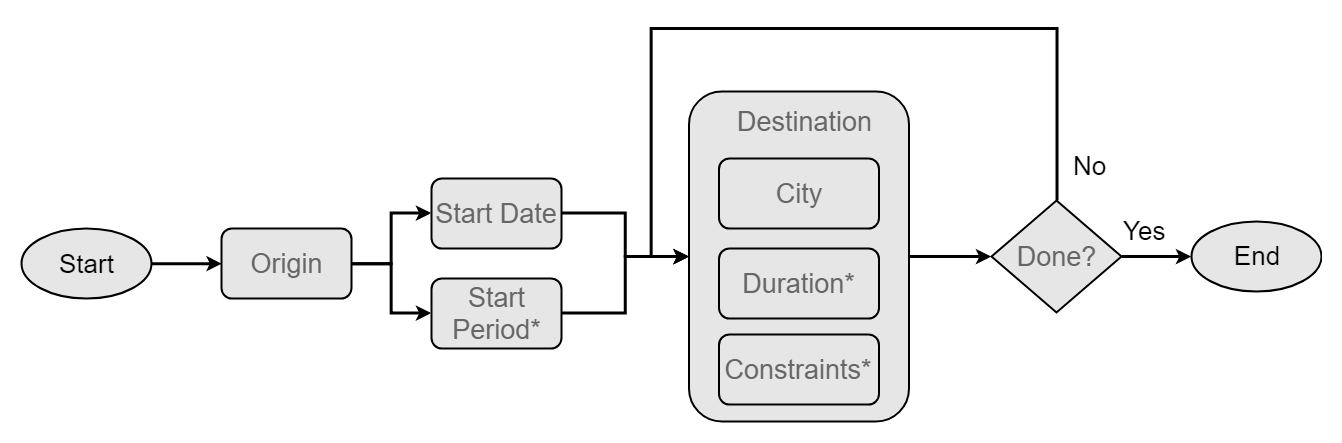
\includegraphics[width=\textwidth]{Figures/system_implementation/user_input.png}
%   \caption{Block diagram of the user input cycle.}
%   \label{fig:user_input}  
% \end{figure}


%_________________ AIRPORT VALIDATION ______________

% Figure of airport validation.
% This is not a central key to the program, so use the image only if we need extra content
% \begin{figure}[H]
%   \centering
%   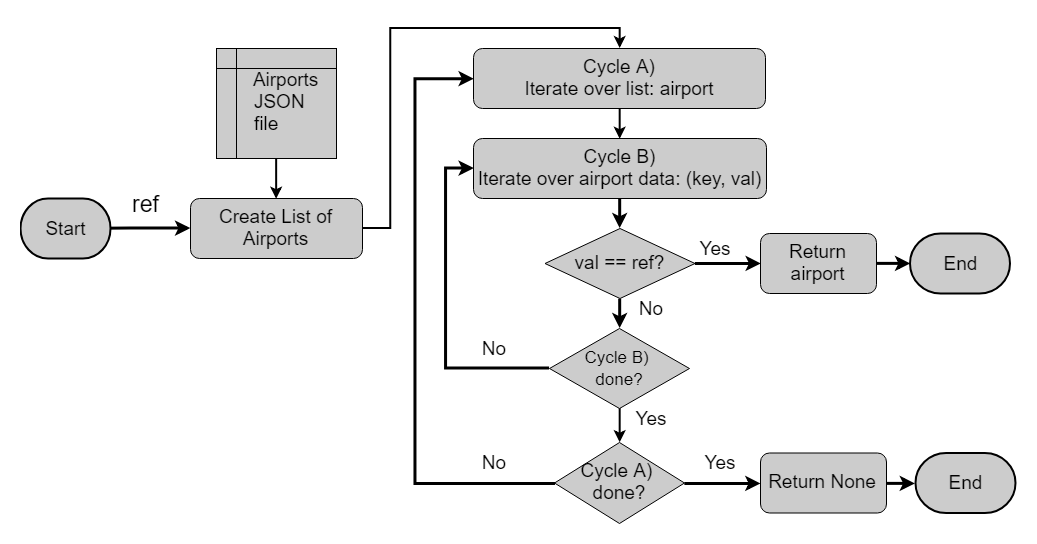
\includegraphics[width=\textwidth]{Figures/system_implementation/airports.png}
%   \caption{Validation of an user introduced airport based on an airport list stored in a JSON file.}
%   \label{fig:airports}  
% \end{figure}

\subsection{Communication with the SSA API}
\label{sec:api_communication}
Upon the construction of a complete request, the Client Side Application 
must call a third-party API to process the request. Since there 
is no apriori information regarding the ammount of time necessary to process the request,
the implementation of this crucial step should be asynchronous.
This means that users can continue to interact with the application, while the request is being processed.

The businnes logic of the developed application is managed by Redux, but Redux by itself is not able
to create asynchronous behaviour. In order to do so, it is necessary to use two secondary libraries:
redux-thunk, and superagent. \textit{Redux-thunk} is a store enhancer, or a middleware,
providing additional functionalities to the store,
and \textit{superagent} is a library for asynchronous javascript and XML (AJAX) requests.

While Redux defines that an action must return a pure javascript object, Redux-thunk overwrites this behaviour,
and lets an action return a function instead. Thus, an asynchronous action 
is an action which upon being completed, invokes a function, which dispatches a secondary action.
This means that an asynchronous action may update the state two times: the first when the action is initially dispatched,
and a second time when the request is complete.
In order to inform the user that the request is being processed, the primary action should 
update the state with some waiting information, while the secondary action interacts with the API.

The details of the asynchronous action previously explained are illustrated in figure \ref{fig:ajax_request}.
Note that an asynchronous request starts with an user defined action, dispatched from inside a component,
and updates the Redux store at two particular moments in time: the first immediatly, and the second after receiving the asynchronous response.

\begin{figure}[htpb]
  \centering
  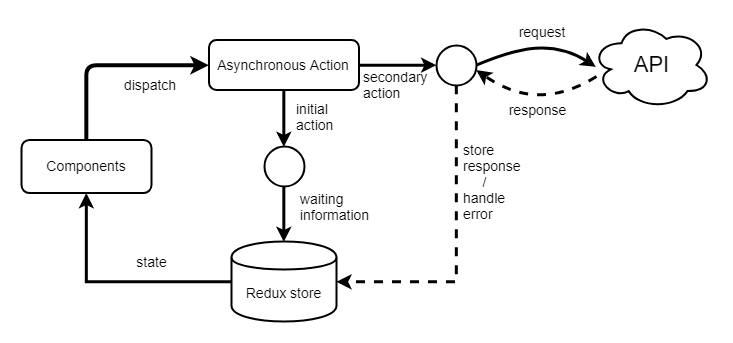
\includegraphics[width=\textwidth]{./Figures/system_implementation/async_request.png}
  \caption{Asynchronous javascript request.}
  \label{fig:ajax_request}  
\end{figure}

The actual request to the third-party API corresponds to a simple HTTP request to a particular URL,
according to the API protocol defined in subsection \ref{sec:api_protocol}. The URL extenstion, called 
the Uniform Resource Identifier (URI), enables the specification of the particular resource under request.
Thus, the URI may be implemented as a way of specifying the attributes which characterize the user selected resource.
It follows thats a particular resource is identified by a collection of (key, value) pairs,
which identify the resource attribute and its user defined value.
There are a total of 7 keys which may be used to construct a request: flyFrom, returnTo, flyTo, startDate, endDate, duration and tripType.


\subsection{User Interface}
\label{sec:user_interface_ready}
This subsection specifies the implementation details of the User Interface,
and should be considered together with figure \ref{fig:UI_views},
which illustrates the design proposed for the application.
The User Interface consists in a single page application,
divided into three main views: the \textit{Request}, \textit{Response} and \textit{Map view}.
Due to the implementation using React, every view is managed by a container,
which reads the state from the store, calls the rendering of presentational components,
and may dispatch actions on user input or other events. 

The User Interface is designed to be mobile friendly, by being responsive to the 
device size. This is achieved using the Bootstrap grid system, 
a website design paradigm in which the user screen is divided into 12 columns,
and each block of the user interface may specify a variable number of columns, depending on the screen size.
The results of this implementation is illustrated in figure \textbf{insert mobile vs desktop figure here}
%\ref{fig:desktop_vs_mobile_app},
where the mobile and desktop versions are put side a side for comparison.

Figure \ref{fig:user_interface_example} is a screenshot of the current version 
of developed application.


\begin{figure}[htpb]
  \centering
  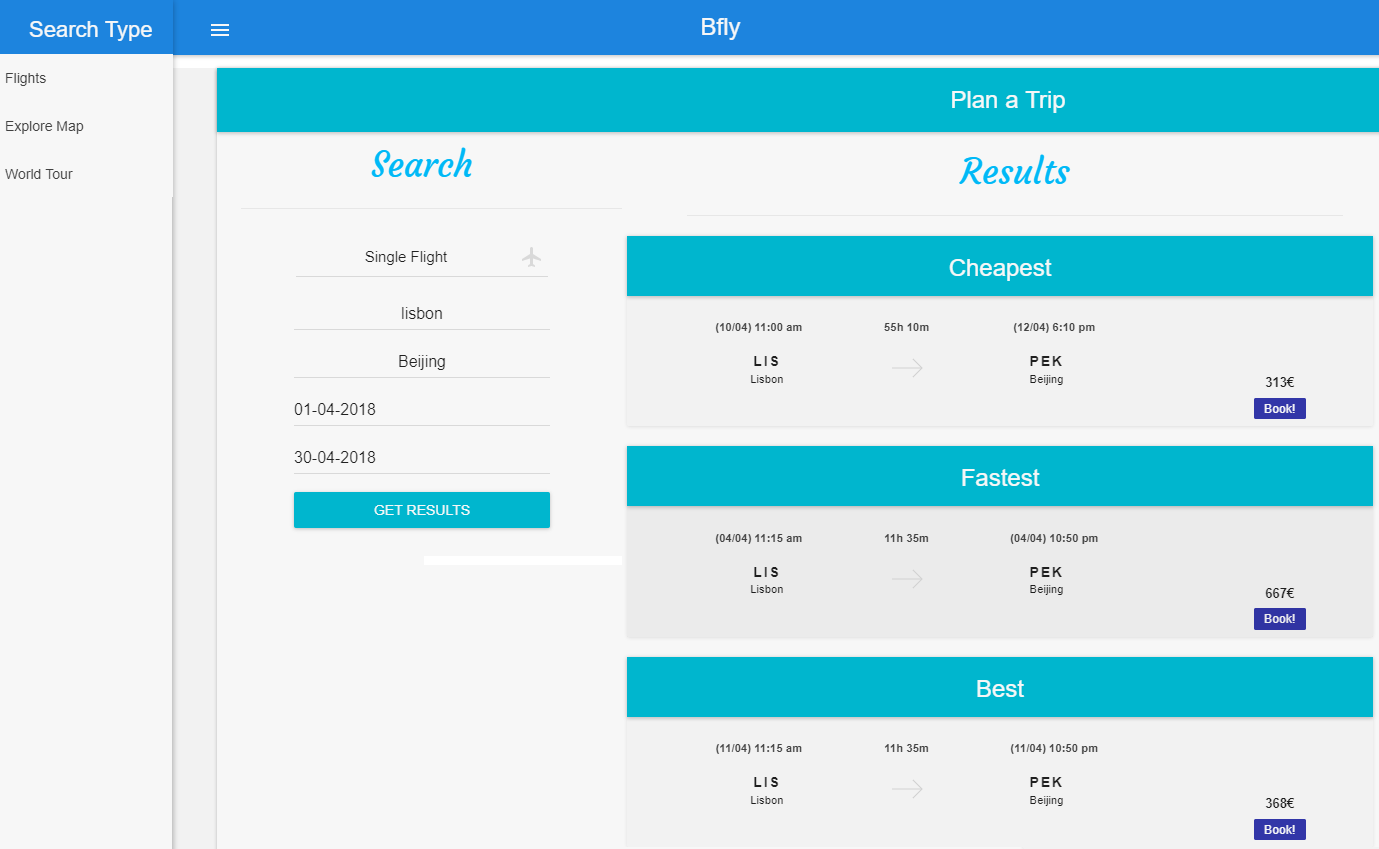
\includegraphics[width=\textwidth]{./Figures/system_implementation/user_interface_example.png}
  \caption{Print screen of the User Interface, as is, displaying the request 
  of a single flight between Lisbon and Beijing, over the span of a month. Three results 
  are presented, the cheapest (313€/55:10h), fastest (667€/11:35h), and most efficient (368€/11:35h) flight.}
  \label{fig:user_interface_example}  
\end{figure}    
\section{Server Side Application}

The Server Side Application is the system responsible for producing a solution to a user request, which corresponds to the specific resources, as described in section \ref{sec:api_protocol}. Producing a solution to a user request involves the communication with third party API's, as to obtain the necessary flight data, which is handled by the Data Management System, detailed in section \ref{sec:dms_implementation}. The actual production of a solution is managed by the Optimization System, as described in chapter \ref{chap:os}. The architecture and implementation details of the SSA are presented in section \ref{sec:api_architecture}.


% \begin{figure}[H]
%   \centering
%   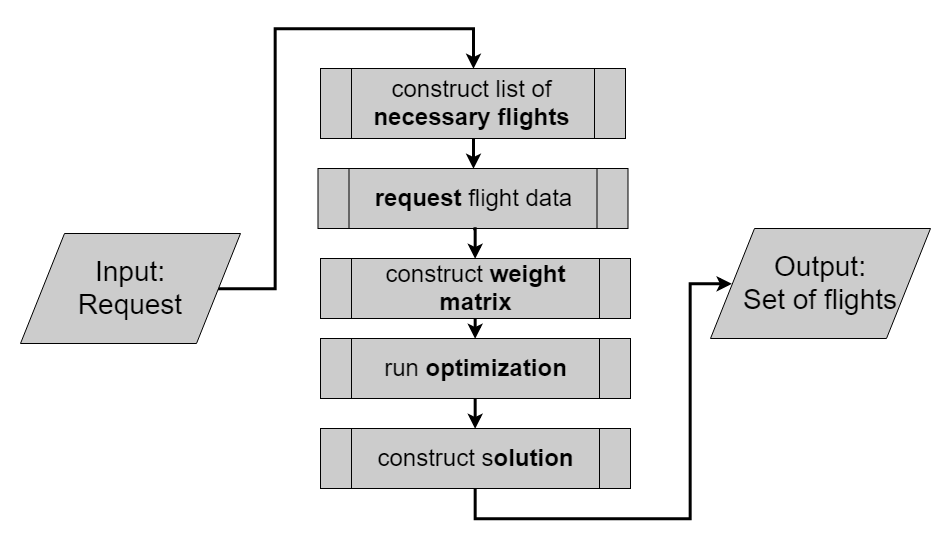
\includegraphics[width=\textwidth]{Figures/system_implementation/overall_flow_2.png}
%   \caption{Necessary steps to construct a solution to a user request.}
%   \label{fig:solution_steps}  
% \end{figure}


\subsection{API architecture}
\label{sec:api_architecture}
\todo{PAREI A REVISAO AQUI.}

The goal of the Server Side Application is to process user defined requests, and to construct a solution to them. There are two steps to produce a response to a request: data collection, and optimization. Both of these steps are managed by the SSA, respectively in the Data Management System (DMS) and in the Optimization System (OS). The data collection procedure will be explained with more detail in subsection \ref{sec:dms_implementation}, while the optimization procedure was described in chapter \ref{chap:os}.

The Server Side Application is built using Python and a Python framework denoted Django, which facilitates the construction of servers and APIs. Django enables the creation of routes for the application, and each of these is connected to a particular set of instructions. It is also possible to define a pattern each route, enabling the setting of user selected input. \todo{shit paragraph}

Upon receiving a request, its Uniform Resource Identifier (URI) is used to identify a particular resource, and the set of user selected input. This data is used as input to a python class called \textit{Resource}. Upon creating the Resource object, the user defined request is validated. In case there is an error in the data, for example a past date, or an invalid airport/city, the proccess does not continue, and Django responds with an error. On the other hand, if the validation is succesfull, the Resource object creates a second class object, called \textit{Request} object. There are 3 types of request objects: the \textit{single}, \textit{round} and \textit{multicity} trip. These objects are not to be confused with the respective single/round flight. While a flight corresponds to a single instance connecting two locations in a particular date, a single/round flight may have an extended start period, in which case there are several flights which may constitute a solution to a user request.

Every Request class has a particular set of functions which are executed each time the class is instantiated. This set of instructions are called the \textit{main} cycle of each request object, and correspond to the:

\begin{enumerate}[noitemsep,topsep=0pt,parsep=0pt,partopsep=0pt]
  \item creation of a list of necessary flights;
  \item acquisition of the necessary flight data;
  \item construction of the weight matrix according to the objective function;
  \item execution of the optimization algorithms;
  \item construction of the solution;
\end{enumerate}

From the above defined main cycle, steps i), iii) and v) are done internally, by each of the class object, while steps ii) and iv) are managed by the Data Management and Optimizaion system, respectively. Note that the step iv), the execution of optimization algorithms, is not necessary for the single/round trip objects,
because the best solution is unambiguous.

Figure \ref{fig:api_structure} illustrates the structure of the Client Side Application. This application is activated each time a request is received, which activates  the instantiation of a \textit{Resource} object, responsible for the validation of the request. After a successfull validation, the Resource object instantiates a \textit{Request} object, which executes the \textit{main cycle} of the solution construction procedure, by first calling the Data Management System to collect the necessary set of flights, following this with the execution of a series of optimization algorithms, to produce a stream of responses which can be served to respond to the request.

\begin{figure}[htpb]
  \centering
  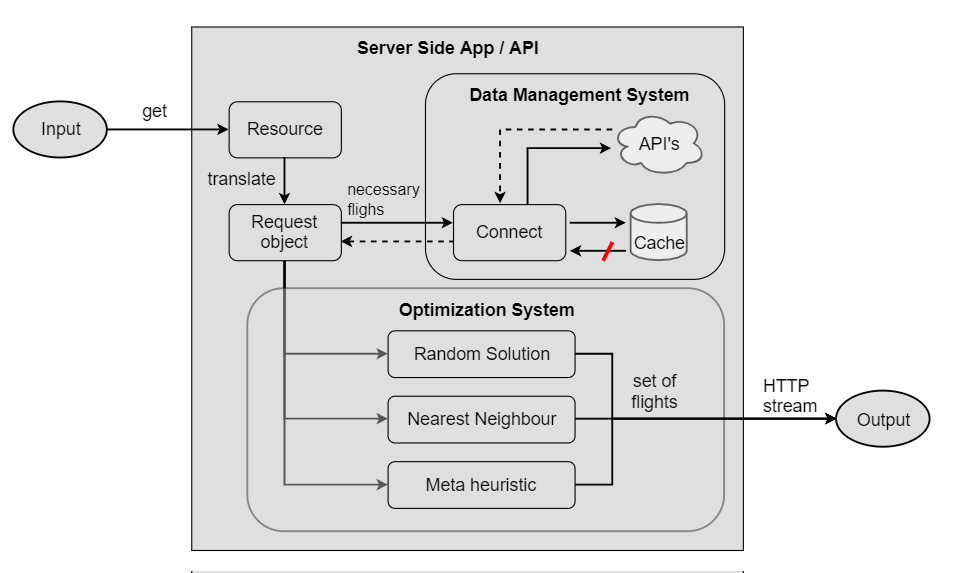
\includegraphics[width=\textwidth]{./Figures/system_implementation/api_structure.png}
  \caption{Structure of the Server Side Application/API.}
  \label{fig:api_structure}  
\end{figure}

\subsection{Api protocol}
\label{sec:api_protocol}
This subsection introduces the syntax of the implemented API protocol. The objective of this protocol is to be simple and clear, and enable an easy interpretation of the user request. \todo{Add footnote with link to API and its documentation}

Every user request may be formullated as a Flying Tourist Problem instance, as proposed in \ref{sec:ftp_design}. Thus, each request is characterized by a limited number of attributes (origin, start date, etc.). This means that the identification of a specific resource can be achieved by including each of these attributes in the uniform resource identifier.

Each request starts with the API endpoint, the specification of the resource type, '/flights', followed by the necessary atributes to describe the requeest. These atributes are grouped using a '\&' symbol, and do not require a specific order. Table \ref{table:api_symbols} \todo{Review table} specifies the possible request attributes, together with the keyword necessary to identify it, and the details and datatype of each.

\begin{table}[]
  \centering
  \caption{This table specified the (keywords, value) pairs, which must be specified in order 
  to uniquely identify a resource.}
  \setlength{\tabcolsep}{3mm}
  \label{table:api_symbols}
  \begin{tabular}{llll}
  \hline
  \\[-0.75em]
  Name         & Symbol     & Keyword                                                       & Details                                                                                                                                                                                   \\
  \\[-0.75em]
  \hline
  \\[-0.75em]
  start city   & $v_0$       & flyFrom=                                                      & Requires a city name, or an ICAO code.                                                                                                                                                    \\
  \\[-0.75em]
  return city  & $v_{n+1}$ & returnTo=                                                     & Requires a city name, or an ICAO code.                                                                                                                                                    \\
  \\[-0.75em]
  destinations & $V$          & cities=                                                       & \begin{tabular}[c]{@{}l@{}}Defines the cities to be visited. \\ Accepts multiple values, sepparated by comma.\\ Each city is specified by a city name or an ICAO code.\end{tabular}       \\
    \\[-0.75em]
  durations    & $D$          & duration=                                                     & \begin{tabular}[c]{@{}l@{}}Defines the duration of stay, in days, for each city.\\ Each value must be a positive integer.\\ Must be the same length as the number of cities.\end{tabular} \\
    \\[-0.75em]
  start date   & $T_0$       & \begin{tabular}[c]{@{}l@{}}minDate =\\ maxDate =\end{tabular} & \begin{tabular}[c]{@{}l@{}}minDate specifies the earliest start date $T_{0i}$,\\ while maxDateidentifies  the max $T_{0f}$. \\ Each date follows the dd/mm/yyyy format.\end{tabular}  \\
    \\[-0.75em]
    \hline
  \end{tabular}
  \end{table}

\subsection{Data Management System}
\label{sec:dms_implementation}
The Data Management System (DMS) is responsible for collecting the set of necessary flights,
in order to process user defined request.
As discussed in section \ref{sec:dms_design}, it is possible to obtain this flight data 
in two distint ways, by using a third-party flight data API, or by performing web scraping.
Both of these methods were implemented and tested, and the results will be discussed in section \textbf{put the section 
of the comparison of API vs webscraping here}. During the development of this work, several API's were tested, and the one which is currently being used
is the \textit{Kiwi.com} API, whose details can be found in the followig website: \textit{https://docs.kiwi.com/}. 


Communicating with a third-party API to request flight data is simply a matter of making HTTP requests
using an URL which defines the resource under query. This request is usually answered with a 
JSON or XML object, which contains the relevant response for the performed request.
In general, each API has its own URL syntax and response structure. Thus, communicating with different 
API's requires the differentiation of the resource identification and response parsing methods,
because these are usually API dependent. 
Thus, communicating with an API usually involves three steps:

\begin{enumerate}[noitemsep,topsep=0pt,parsep=0pt,partopsep=0pt]
  \item creation of a URL specifying the intended resource;
  \item execution of an HTTP request to the URL;
  \item deconstruction (parsing) of the response;
\end{enumerate}

These three essential steps are the base for any data collection system. They can be used to collect data from an API,
and they can also be used to do webscraping. In general, the difference between these two methods (api vs webscraping)
is more likely to be felt in the parsing of the response. Using an API,
the response is usually structured and organized, encoded in a JSON data type, or similar,
which is, in general, human readable.
In its turn, using web scraping, the response comes in the form of HTML, and the necessary data 
may be trapped under many levels of HTML objects. In general, it is harder to parse the result of webscraping.

There is a second difference that must be mentioned when comparing the usage of API's and webscraping.
Webscraping is the act of retrieving the data visible on the \textit{screen}.
The problem is that, in many cases, before the data becomes visable, 
javascript has to be executed, and in some cases, there are database acceses,
which usually require a substaintial ammoun of time to execute.
In this case, it is said that the websites uses javascript to render their page, and
in general, webscraping javascript websites is much more harder
and slower, because a simple HTTP request is not sufficient to obtain the necessary data.
Instead, it is necessary to emulate a browser,
make the HTTP request, and wait for the javascript to be completly loaded.
During the development of this system, the \textit{httplib} module of the python programming language
was utilized for executing the HTTP requests,
and the \textit{Selenium Web driver} library for the execution of a automatable browser.

Given a list of flights whose data must be collected,
figure \ref{fig:serial_api} illustrates the necessary steps to communicate 
with a thid-party API, using HTTP protocol, to obtain the necessary data.
In this figure, the system utilizes a serial approach, which means that at any time,
only one request is being executed. 

\begin{figure}[htpb]
  \centering
  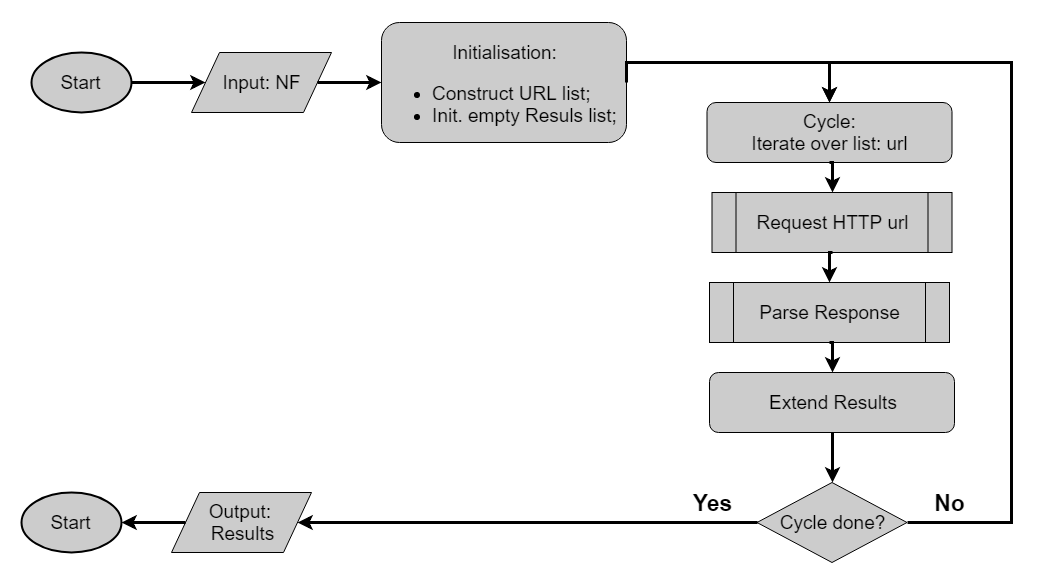
\includegraphics[width=\textwidth]{./Figures/system_implementation/serial_api.png}
  \caption{Communication with third-party API's, using HTTP protocol, and a serial requesting scheme.}
  \label{fig:serial_api}  
\end{figure}

The bottleneck of the serial system illustrated in figure \ref{fig:serial_api},
is the necessary time to receive the response to an HTTP request.
In order to take advantage of this bottleneck, a concurrent approach was considered,
in which the waiting period of a request is utilized to spwan more requests.
This approach is achieved by adopting a \textit{Producer-Consumer} system,
illustrated in figure \ref{fig:concurrent_api}. This system 
spwans at most $n_{max}$ threads (workers),
one at a time, to execute a list of jobs, which correspond 
to making an HTTP request and parsing the response.
Using this approach, the bottleneck experienced by each worker 
is not imposed on any of the other $n_{max} -1$ workers,
and thus the time-delay is not cummulative.


\begin{figure}[htpb]
  \centering
  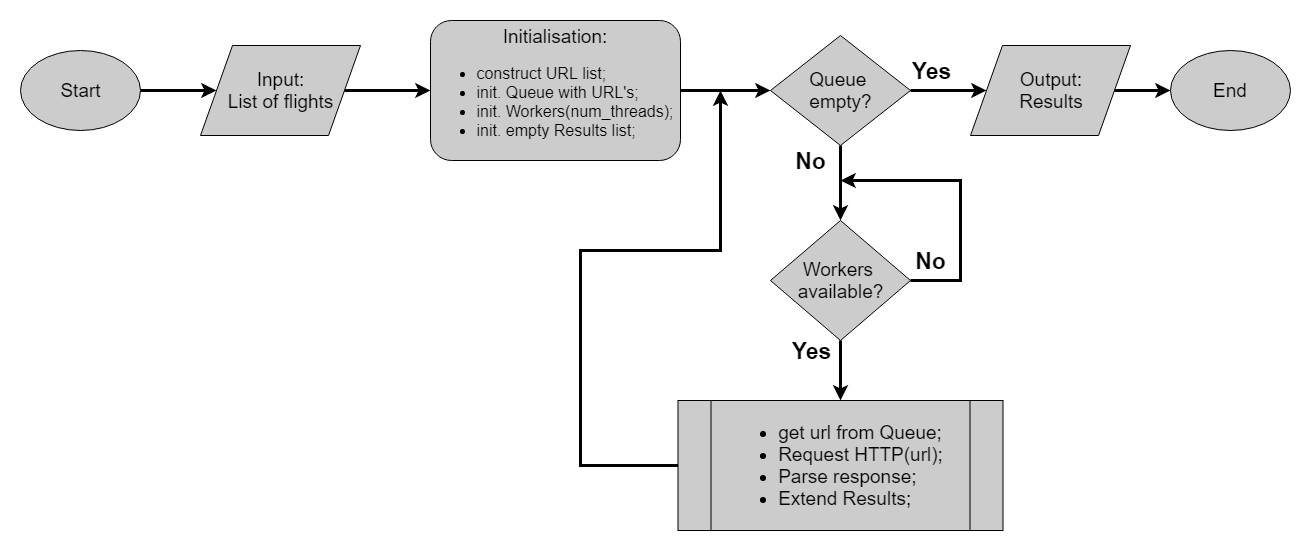
\includegraphics[width=\textwidth]{./Figures/system_implementation/concurrent_api.png}
  \caption{Communication with third-party API's, using HTTP protocol, and concurrent requesting scheme to take advantage of the waiting times.}
  \label{fig:concurrent_api}  
\end{figure}


The webscraping systems developed are very similar to those illustrated in figures \ref{fig:serial_api} and \ref{fig:concurrent_api}.
However, instead of making simple HTTP requests, a Selenium browser is used to access the website.
Consequentially, the execution of the concurrent approach must create, at most, $n_{max}$ browsers.
The illustration of these systems may be consulted in the \textbf{ANEXO}.

Subsection \textbf{section herereeere} will evaluate the proposed system,
and compare the efficiency of the serial and concurrent approaches,
for both the API collectiong and the webscraping. These two systems will also be compared 
in order to evaluate which is most adequate for the usage in a production system.



    
%\cleardoublepage
%Chapter 7
\acresetall
\fancychapter{Experimental Results}
\label{cap:ER}

In order to validate and evaluate the performance of the developed system, several tests were developed and executed. First, by using a set of benchmarks, the implemented optimization algorithms are tested as to evaluate their overall quality (section \ref{sec:os_eval}). Then, the overall utility of the proposed system is evaluated, by performing a series of tests on the Flying Tourist Problem (section \ref{sec:ftp_eval}). Finally, a thorough comparison with the only known state-of-the-art alternative for the devised FTP is performed (section \ref{sec:nomad}). This is achieved by considering a comprehensive set of real-world multi-city flight problems, using different objective functions as to evaluate the systems performance.

These experiments were executed on a 2.6GHz Intel i7-6700 CPU, with 8GB of RAM, and all the code was developed using the Python3 programming language. 
%In particular, the quality of the obtained solutions are compared with those provided by the \textit{metric nearest neighbor} heuristic, which promotes the nodes proximity to define the traveling route and closely approximates the strategy usually adopted by a human solver.


\section{Optimization module evaluation}
\label{sec:os_eval}

The main difficulty behind the aimed evaluation of the developed optimization module results from the absence of publicly available FTP benchmarks (with \textit{a priori} known optimal solutions) that could be used to validate the obtained results. To circumvent this adversity, it was decided to conduct such evaluation using closely-related NP-hard problems, such as the  Asymmetric TSP (subsection \ref{sec:atsp_eval}) and Time-Dependent TSP  (subsection \ref{sec:tdtsp_eva}).

%% Asymmetric TSP problem
%% ________________________
\subsection{Asymmetric TSP evaluation}
\label{sec:atsp_eval}

The set of benchmarks (and respective input data) considered for the Asymmetric TSP were collected from the publicly available TSPLib and correspond to problems with 17, 35, 53, 124 and 323 nodes (br17, ftv35, ft53, kro124p, rbg323, respectively). The adoption of such graph dimension ranges allows the evaluation of the developed optimization module with different complexity levels: small instances (17 nodes), corresponding to a dimension more closely-related to the targeted \textit{flying tourist} application scenario; medium instances (35-53 nodes), used to evaluate more computationally demanding scenarios; and large instances (124-323 nodes), used to evaluate the scalability of the developed system.

Each benchmark was independently solved by the two considered optimization algorithms (ACO and SA). The execution of each problem was repeated 5 times and the obtained results were averaged.  

Furthermore, since there are strict limitations on the maximum time a user is willing to wait for a result in a real-world application, it was considered a stop criteria to limit the total optimization time. In accordance, during the execution of these tests, each algorithm may run for no longer than 60 seconds. 
The results of both meta-heuristic algorithms on the considered set of asymmetric benchmarks are presented in Table~\ref{tab:tsp_results}. 

\begin{table}[b]
\centering
\caption{Performance of the ACO and SA on the asymmetric TSP benchmarks, taken from the TSPLib (stop-criteria = 60 seconds). }
\label{tab:tsp_results}
\begin{tabular}{@{}l l c c c c c@{}}
\hline
\multirow{2}{*}{Alg.}& Bench   & \multirow{2}{*}{\#Iterat.}  & Optimal  & Comput.  & Error  \\ 
                     & mark    &                             & solution & solution &  [\%]  \\ \hline
\multirow{5}{*}{ACO} & br17    & 6893    & 39        & 39       & 0              \\  
                     & ftv35   & 1469    & 1473      & 1552.4   & 5.39         \\  
                     & ft53    & 689     & 6905      & 8269.6   & 16.13        \\ 
                     & kro124p  & 275     & 36230     & 44102    & 17.00         \\   
                     & rbg323  & 20      & 1326      & 1660.4   & 25.21      \\ \hline
\multirow{5}{*}{SA}  & br17    & 264319  & 39        & 39       & 0               \\  
                     & ftv35   & 63659   & 1473      & 1641		& 11.41       \\  
                     & ft53    & 36189   & 6905      & 7963     & 15.32        \\  
                     & kro124p  & 17533    & 36230     & 44102   & 21.73      \\  
                     & rbg323  & 1361    & 1326      & 1706.2   & 28.67        \\ \hline
\end{tabular}
\end{table}

For small instances (17 nodes), both ACO and SA consistently present optimal solutions. For medium instances (35-53 nodes), both algorithms perform in the range of 5-16$\%$ relative error. As for bigger problems (124-323 nodes), the performance of the ACO slightly decreases (17-25\%), followed closely by the SA (22-29\%). 

By observing the number of iterations that were executed during the 60-seconds interval, it is clear that the SA is much faster than the ACO, performing 38 to 68 times more iterations in the same time interval. However, this greater number of iterations does not seem to directly contribute to a better final result of the SA. This happens because the ACO search strategy is guided, taking into account the previous search experience in the selection of the next solution. This does not occur with the classical implementation of the SA, which utilizes a simple and non-guided local search.

On the other hand, while the considered stop-criteria value may be sufficient to reach the metaheuristic stationary result for small problem instances, meaning that continuing the optimization further may not affect the final error in a significant way, the higher relative error and lower number of iterations for bigger problem instances suggest that improvements may still occur.%the stagnation was not yet reached. 

To analyze the advantages of further optimization, all problems were solved once more, by using the same procedure previously described, this time for a total of 300 seconds. The obtained results are presented in Table~\ref{tab:further_opt}, which allow the comparison of the final result as a function of the execution time. Columns RE60 and RE300 present the relative error after 60 and 300 seconds, respectively. As it can be seen, increasing the optimization time leads to an improvement in the final result for both metaheuristics and for almost every benchmark problem. These improvements are more significant for bigger problem instances, and affect the small instances only slightly.

Hence, the observed performance of the implemented metaheuristic algorithms on the asymmetric TSP, for the level of complexity of the targeted \textit{flying tourist} application scenario, showed to be highly promising, leading to final solutions which are either optimal or whose relative error is close to 10\%. \todo{Review paragraph}

\begin{table}[t]
\centering
\caption{Effects of increased optimization time on the final result.}
\label{tab:further_opt}
\begin{tabular}{ccccc}
\hline
         & \multicolumn{2}{c}{ACO} & \multicolumn{2}{c}{SA} \\
Benchmark & RE60      & RE300      & RE60       & RE300      \\ \hline
br17     & 0          & 0          & 0         & 0          \\
ftv35    & 5.39       & 4.75           & 11.41     & 11.73      \\
ft53     & 16.13      & 13.71 			& 15.32     & 13.20      \\
kro124p   & 17.00       & 13.91            & 21.73     & 17.21      \\
rbg323   & 25.21      & 18.78            & 28.67     & 10.27      \\
\hline
\end{tabular}
\end{table}



\subsection{Time-dependent TSP evaluation}
\label{sec:tdtsp_eva}

Due to the absence of standardized benchmarks for the time-dependent case in the TSPLib, it was necessary to define specific problems (whose best known solutions are known \textit{a priori}) by using a method described in (\cite{TDTSP_construction}), based on the duality principle over the Integer Linear formulation for the time-dependent TSP. The defined benchmarks were constructed as to have the same dimensions of those used for the Asymmetric TSP, and their names were appended with an asterisk suffix to distinguish from the asymmetric TSP case.

Executing the same evaluation strategy on the time-dependent TSP problems leads to the results presented in Table~\ref{tab:tdtsp_results}. Once again, it is possible to compare the efficiency of the ACO and the SA, by evaluating the relative error of each set of problems.

\begin{table}[b]
\centering
\caption{Performance of the ACO and SA on the time-dependent TSP benchmarks (stop-criteria = 60 seconds).}
\label{tab:tdtsp_results}
\begin{tabular}{@{}l l@{}c c c c c@{}}
\hline
\multirow{2}{*}{Alg.}& Bench   & \multirow{2}{*}{\#Iterat.}  & Optimal  & Comput.  & Error  \\ 
                     & mark    &                             & solution & solution &  [\%]  \\ \hline
\multirow{5}{*}{ACO} & br17*    & 9720    & 2458        & 2729                 & 11.03          \\  
                     & ftv35*   & 2590    & 5131       & 5500              & 7.20       \\  
                     & ft53*    & 1099     & 7930      & 8370               & 5.53      \\ 
                     & kro124p*  & 71     & 25483     & 26402         & 3.61     \\   
                     & rbg323*  & 13      & 48991      & 50261                & 2.59      \\ \hline
\multirow{5}{*}{SA}  & br17*    & 219517  & 2458        & 2631             & 7.04          \\  
                     & ftv35*   & 80262   & 5131      & 5406			  & 5.38      \\  
                     & ft53*    & 37450   & 7930      & 8265           & 4.23      \\  
                     & kro124p*  & 3521    & 25483     & 26427         & 3.70     \\  
                     & rbg323*  & 901    & 48991      & 51926              & 5.99      \\ \hline
\end{tabular}
\end{table}

For small instances (17 nodes), ACO and SA present a small relative error, ranging from 7\% and 11\%. For medium instances (35-53 nodes), the relative error decreases for both algorithms, ranging from 4\% to 7\%, with SA offering better results than ACO. This may occur because the high number of performed iterations in small and medium instances leads to an intensive search space exploration. However, when  bigger problems (124-323 nodes) are considered, the performance of the ACO increases (possibly due to its guided search exploration), reducing the relative error to close to 3\% and surpassing that of the SA.

In any case, the performance of these two algorithms on the time-dependent TSP is highly promising, leading to final solutions which are consistently below the 10\% relative error mark. 

A precise interpretation of the factors involved in these results is hard. Still the following conclusions seem plausible. When comparing the time-dependent TSP with the asymmetric TSP we usually expect the former to be more heavily constrained than the latter. In those cases finding the problem itself simplifies finding the overall optimum, as bad solutions are much easier to identify. In particular both ACO and SA seem to explore this property well, as can be inferred by the fact that for the corresponding benchmarks the time dependent version obtains a better relative error rate with less iterations. Moreover we believe that the better relative error rates themselves are also problem induced, meaning that the asymmetric TSP contains big gaps in the objective function, in particular from the optimal value to a close by maximum, whereas the time-dependent TSP contains smaller gaps and a higher concentration of near maximums. \todo{Review paragraph}



% \begin{table*}[]
% \centering
% \caption{Performance of the optimization algorithm on the \textbf{time-dependent TSP}.}
% \label{tab:tdtsp_results}
% \begin{tabular}{|l|l|l|l|l|l|}
% \hline
% algorithm            & problem & opt cost & meta cost & num. iterations & rel. error \\ \hline
% \multirow{5}{*}{SA}  & p17     & 2458     & 2631.2    & 219517.2        & 7.04       \\ \cline{2-6} 
%                      & p35     & 5131     & 5406.8    & 80262           & 5.38       \\ \cline{2-6} 
%                      & p53     & 7930     & 8265.6    & 37450.6         & 4.23       \\ \cline{2-6} 
%                      & p170    & 25483    & 26427     & 3521            & 3.70       \\ \cline{2-6} 
%                      & p323    & 48991    & 51926.8   & 900.6           & 5.99       \\ \hline
% \multirow{5}{*}{ACO} & p17     & 2458     & 2729      & 9720.6          & 11.03      \\ \cline{2-6} 
%                      & p35     & 5131     & 5500.2    & 2590.6          & 7.20       \\ \cline{2-6} 
%                      & p53     & 7930     & 8370.4    & 1099.6          & 5.53       \\ \cline{2-6} 
%                      & p170    & 25483    & 26402.4   & 71.2            & 3.61       \\ \cline{2-6} 
%                      & p323    & 48991    & 50261.4   & 13.4            & 2.59       \\ \hline
% \end{tabular}
% \end{table*}

\section{Flying Tourist Problem evaluation}
\label{sec:ftp_eval}

To demonstrate and quantify the actual benefits of the proposed system, a series of FTP instances were defined, ranging from just 1 city to visit (which corresponds to a round-tri[), up to a total of 20 cities. For each problem instance, several solutions were obtained using four different approaches:
\begin{itemize}
    \item a \textit{pseudo-random} approach, i.e., a closed tour randomly generated that connects all the ;
    \item a \textit{metric nearest-neighbor} heuristic that promotes the nodes proximity to define the traveling route (this approach closely approximates the strategy usually followed by a human solver);
    \item a \textit{regular nearest-neighbor} heuristic using the flight price as the objective function;
    \item the \textit{proposed ACO and SA} meta-heuristics (where the best of these two results is chosen), considering two different objective functions (minimization of the total cost and of the entropy). 
\end{itemize}  

In this experiment, the number of nodes was varied and multiple requests (more than 5) were made for each set of nodes, averaging their results.
In every case, the trip starts and returns to Lisbon (Portugal) and visits a given set of cities, randomly chosen from the following set: 
Abuja, Atlanta, Barcelona, Beijing, Cairo, Casablanca, Dubai, Dublin, Frankfurt, Hong Kong, Istanbul, 
Johannesburg, Kiev, Los Angeles, Madrid, Miami, Moscow, New-York (JFK), Oslo, San Francisco, Sidney, Singapore. The start date was set to be the same for all requests(\textit{1 November 2018}), which, upon the execution of the tests, was 50 days into the future. The waiting period on each city was set to a random value between 1 and 5 days. 


%________________________________________________________________________________________________
%_____________________________ Quantitative evaluation ____________________________________________
%________________________________________________________________________________________________
\subsection{Quantitative evaluation and improvement}
\label{sec:ftp_quantitative_eval}

\begin{table*}
\definecolor{Gray}{gray}{0.9}
\definecolor{green}{rgb}{0,0.5,0}
\definecolor{red}{rgb}{0.75,0,0}
\setlength\tabcolsep{4pt}
\renewcommand{\arraystretch}{1.25}
\centering
\caption{Comparison of different Flying Tourist Problem solutions obtained with distinct algorithms and optimization criteria, considering the \textit{Metric Nearest Neighbor} approach (shaded gray) as reference.} 
\resizebox{1.0\textwidth}{!}{
  \begin{tabular}{l|l|r@{~}r|r@{~}r|r@{~}r|r@{~}r|r@{~}r|r@{~}r|r@{~}r|}
  \label{tab:utility}
                                     & \multicolumn{1}{r}{\#Nodes} 
                                     & \multicolumn{2}{|c}{1} 
                                     & \multicolumn{2}{|c}{3}    
                                     & \multicolumn{2}{|c}{5}    
                                     & \multicolumn{2}{|c}{7}
                                     & \multicolumn{2}{|c}{10}   
                                     & \multicolumn{2}{|c}{15}
                                     & \multicolumn{2}{|c|}{20}   \\
  \hline  
  \multirow{4}{*}{\begin{sideways}\hspace*{-4ex}\textbf{PRICE}\end{sideways}}     
                    & Random            & 635  & 
                                                & 1455 & {\color{red}(+1.2\%)} 
                                                & 2194 & {\color{red}(+7.0\%)} 
                                                & 3436 & {\color{red}(+26.6\%)} 
                                                & 4791 & {\color{red}(+28.8\%)} 
                                                & 7222 & {\color{red}(+63.5\%)} 
                                                & 9154 & {\color{red}(+68.8\%)} \\
                    & \cellcolor{Gray}Metric Nearest Neighbor   
                                                & \cellcolor{Gray}635  & \cellcolor{Gray}
                                                & \cellcolor{Gray}1438 & \cellcolor{Gray}
                                                & \cellcolor{Gray}2051 & \cellcolor{Gray}
                                                & \cellcolor{Gray}2715 & \cellcolor{Gray}
                                                & \cellcolor{Gray}3721 & \cellcolor{Gray}
                                                & \cellcolor{Gray}4417 & \cellcolor{Gray}
                                                & \cellcolor{Gray}5422 & \cellcolor{Gray} \\
                    & Regular Nearest Neighbor  & 635  & 
                                                & 1438 & 
                                                & 1993 & {\color{green}(-2.8\%)} 
                                                & 2553 & {\color{green}(-6.0\%)}
                                                & 3412 & {\color{green}(-8.3\%)}
                                                & 3911 & {\color{green}(-11.5\%)}
                                                & 4678 & {\color{green}(-13.7\%)} \\
                            & Proposed (Price)   & 635  & 
                                                & 1398 & {\color{green}(-2.8\%)}
                                                & 1727 & {\color{green}(-15.8\%)}
                                                & 1911 & {\color{green}(-29.6\%)}
                                                & 2466 & {\color{green}(-33.7\%)}
                                                & 3051 & {\color{green}(-30.9\%)}
                                                & 3699 & {\color{green}(-31.8\%)} \\
                            & Proposed (Entropy)& 876 & {\color{red}(+38.0\%)} 
                                                & 1761 & {\color{red}(+22.5\%)}
                                                & 2203 & {\color{red}(+7.4\%)}
                                                & 2749 & {\color{red}(+1.3\%)}
                                                & 3687 & {\color{green}(-0.9\%)}
                                                & 4123 & {\color{green}(-6.7\%)}
                                                & 4707 & {\color{green}(-13.2\%)} \\ \hline
  \multirow{4}{*}{\begin{sideways}\hspace*{-4ex}\textbf{DURATION}\end{sideways}} 
                            & Random            & 61   & 
                                                & 125  & {\color{red}(+5.0\%)} 
                                                & 183  & {\color{red}(+3.4\%)} 
                                                & 270  & {\color{red}(+31.7\%)} 
                                                & 369  & {\color{red}(+48.2\%)} 
                                                & 497  & {\color{red}(+63.0\%)} 
                                                & 638  & {\color{red}(+92.7\%)}  \\
                            & \cellcolor{Gray}Metric Nearest Neighbor        
                                                & \cellcolor{Gray}61 & \cellcolor{Gray}
                                                & \cellcolor{Gray}119 & \cellcolor{Gray}
                                                & \cellcolor{Gray}177 & \cellcolor{Gray}
                                                & \cellcolor{Gray}205 & \cellcolor{Gray}
                                                & \cellcolor{Gray}249 & \cellcolor{Gray}
                                                & \cellcolor{Gray}305 & \cellcolor{Gray}
                                                & \cellcolor{Gray}331 & \cellcolor{Gray}  \\
                            & Regular Nearest Neighbor       & 61 & 
                                                & 119 & 
                                                & 181 & {\color{red}(+2.3\%)}
                                                & 212 & {\color{red}(+3.4\%)}
                                                & 257 & {\color{red}(+3.2\%)}
                                                & 323 & {\color{red}(+5.9\%)}
                                                & 358 & {\color{red}(+8.2\%)}  \\
                            & Proposed (Price)   & 61 & 
                                                & 121 & {\color{red}(+1.7\%)}
                                                & 151 & {\color{green}(-14.7\%)}
                                                & 179 & {\color{green}(-12.7\%)}
                                                & 258 & {\color{green}(+3.6\%)}
                                                & 292 & {\color{green}(-4.3\%)}
                                                & 319 & {\color{green}(-3.6\%)}  \\
                            & Proposed (Entropy)& 29 & {\color{green}(-52.5\%)}
                                                & 57 & {\color{green}(-52.1\%)}
                                                & 82 & {\color{green}(-53.7\%)}
                                                & 92 & {\color{green}(-55.1\%)}
                                                & 104 & {\color{green}(-58.2\%)}
                                                & 140 & {\color{green}(-54.1\%)}
                                                & 160 & {\color{green}(-51.7\%)} \\ \hline 
  \end{tabular}
}
\end{table*}

The result of the execution of the described test is summarized in Table~\ref{tab:utility}, where both the total flight cost and duration are presented, as a function of the optimization approaches and the number of nodes. This table also presents the observed improvement, relative to the \textit{metric nearest-neighbor} solution, which is used as reference due to its proximity to the human search approach.

%\begin{table}[]
%\centering
%\caption{Solving the Flying Tourist Problem with different algorithms and optimization criteria.} 
%\resizebox{0.5\textwidth}{!}{
%  \begin{tabular}{l|c|cccccccccc}
%  \label{tab:utility}
%  \hline
%                            & N & 1    & 3    & 5    & 7    & 10   & 15   & 20   \\
%  \hline
%  \multirow{4}{*}{C}     & R         & 838  & 1520 & 2089 & 3571 & 4819 & 7289 & 9188 \\
%                            & NN        & 838  & 1512 & 1993 & 2479 & 3229 & 3808 & 4665 \\
%                            & MC        & 838  & 1458 & 1655 & 1928 & 2468 & 3104 & 3721 \\
%                            & ME        & 1158 & 1828 & 2124 & 2521 & 3212 & 3996 & 4704 \\ \hline
%  \multirow{4}{*}{D} & R         & 82   & 125  & 194  & 268  & 378  & 518  & 666  \\
%                            & NN        & 82   & 118  & 157  & 203  & 256  & 313  & 344  \\
%                            & MC        & 82   & 111  & 157  & 181  & 267  & 260  & 325  \\
%                            & ME        & 37   & 58   & 63   & 90   & 105  & 142  & 163 \\ \hline 
%  \end{tabular}
%}
%\end{table}


%\begin{table}[]
%\centering
%\caption{Relative improvement of different optimization algorithms compared to random solution.} 
%\resizebox{0.5\textwidth}{!}{
%    \begin{tabular}{c|c|ccccccc}
%    \label{tab:improvement}
%    \hline
%                       & num nodes & 1     & 3     & 5     & 7     & 10    & 15    & 20    \\
%    \hline
%    \multirow{3}{*}{C} & NN        & 0,0   & -0,5  & -4,6  & -30,6 & -33,0 & -47,8 & -49,2 \\
%                       & MC        & 0,0   & -4,1  & -20,8 & -46,0 & -48,8 & -57,4 & -59,5 \\
%                       & ME        & 38,2  & 20,3  & 1,7   & -29,4 & -33,3 & -45,2 & -48,8 \\ \hline
%    \multirow{3}{*}{D} & NN        & 0,0   & -5,6  & -19,1 & -24,3 & -32,3 & -39,6 & -48,3 \\
%                       & MC        & 0,0   & -11,2 & -19,1 & -32,5 & -29,4 & -49,8 & -51,2 \\
%                       & ME        & -54,9 & -53,6 & -67,5 & -66,4 & -72,2 & -72,6 & -75,5 \\ \hline 
%    \end{tabular}
%}
%\end{table}

The first insight into these results allows a preliminary evaluation of the utility of the proposed system. It can be seen that, for a small number of nodes (1 and 3), the \textit{metric} and \textit{regular} nearest neighbour present the same results. However, for greater instances (5-20) nodes, the \textit{metric} nearest neighbour starts to present worse results when compared to the \textit{regular} variant. The \textit{regular} variant performs better (reducing the cost between $\approx$ $3\%$ and $13\%$) because it always selects the node with the lowest cost. Despite the positive results presented by the \textit{regular} nearest neighbour approach, the proposed meta-heuristics are still capable of improving them. The metaheuristic approach enables the cost to be reduced by an extra 3\% to 25\%, when compared to the \textit{regular} nearest neighbour, and up to a total of 34\%, when compared to the \textit{metric} one. 

%The first insight into these results allows a preliminary evaluation of the utility of the proposed system. It can be seen that, for a small number of nodes (1 and 3), there is no significant improvement relative to the \textit{metric nearest-neighbor} solution. However, when greater instances (5-20 nodes) are considered, this straightforward approach stops presenting good results, while its regular variant (using the flight prices objective function) and the proposed meta-heuristics greatly improve the total flights cost ($\approx$ 3-34\%). However, despite the good results that were presented by the regular nearest neighbour approach (using the flight prices), the proposed meta-heuristics are still capable of improving them ($\approx$ 3-25\%).    


\subsection{Balancing the total flight price and duration}
\label{sec:ftp_obj_func_eval}

It is possible to execute the proposed metaheuristics with different objective functions, as proposed in subsection \ref{sec:ftp}. In particular, it is possible to introduce both the price and flight duration in the objective function (see equation \ref{eq:obj_entropy}). With this approach, a better balance between price and flight duration is envisaged, by minimizing an \textit{entropic} metric defined as a weighted value, where the price and flight duration contribute with 70\% and 30\%, respectively.

%Another implementation of the proposed metaheuristics was also considered that introduce the flight duration in the objective function. With such an alternative implementation, it was envisaged a better balance between price and flight duration, by minimizing an entropy metric defined as a weighted value where the price and flight duration contribute with 70\% and 30\%, respectively.

As it can be observed in Table~\ref{tab:utility}, such an \textit{entropic} minimization leads to significant improvements in the flight duration, although it introduces some penalization in the flight price for a small number of nodes (1-5). However, as the number of nodes increases, the flight price significantly decreases, but it is always higher than that provided by the former price-only meta-heuristics. This happens because the two objective functions (price and duration) can hardly be simultaneously minimized, and thus, a compromise has to be reached. In this case, compromising means slightly increasing the price, to significantly reduce the duration.

This compromise between flight price and duration is also illustrated in Fig.~\ref{fig:cost_vs_time}, which presents the relative duration improvement as a consequence of the increase in price. This figure shows that, in general, increasing the price by around 20\% leads to a decrease in the flight duration by around 50\%, when compared to the price-only metaheuristic approach.

\begin{figure}
  \centering
  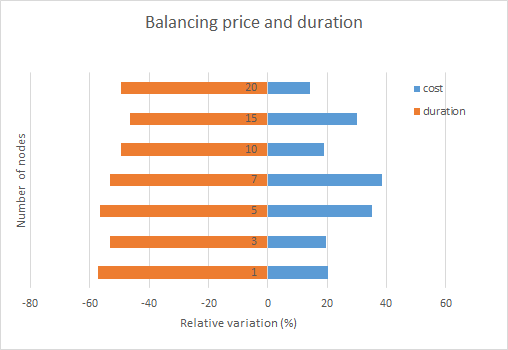
\includegraphics[width=9cm]{./imgs/cost_vs_time.png}
  \caption{Variation of the total flight price and duration when minimizing the entropy objective function.}
  \label{fig:cost_vs_time}  
\end{figure}


\subsection{Impact of the trip start interval}
\label{sec:start_impact}

To evaluate the influence of the trip start interval on the obtained results, the same queries and data sets were used to solve these FTPs using start periods of different lengths.
These results are illustrated in Fig.~\ref{fig:cost_vs_start_period}, where $NN$ refers to the \textit{metric nearest neighbour} heuristic and $M-1$, $M-15$ and $M-31$ represents the proposed meta-heuristic algorithms, with start periods of length 1, 15 and 31 days, respectively. 

The analysis of Fig.~\ref{fig:cost_vs_start_period} shows that increasing the interval of the start date may lead to great improvements, with flight price reductions as high as 15\%, even for medium size instances with up to 20 nodes.  

\begin{figure}[h]
  \centering
  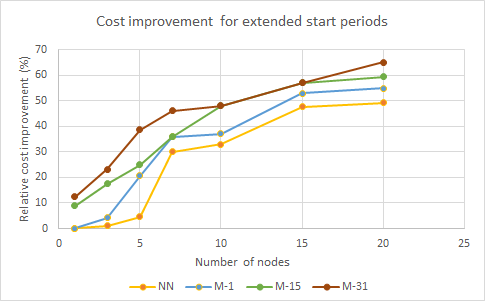
\includegraphics[width=9cm]{./imgs/cost_improvement_startdates.png}
  \caption{Price improvement as a function of the trip start interval.}
  \label{fig:cost_vs_start_period}  
\end{figure}


\subsection{Response time}
\label{sec:response_time}

The response time to a requests depends mostly on two difference procedures: $i$) the data gathering, which is handled by the DMS; and $ii$) the optimization, handled by the OS. This subsection evaluates the response time to a given request, by comparing the relative influence of these two steps. 

As to collect the necessary flight data to a request, it is necessary to communicate with third-party APIs. The module responsible for this is the DMS, which implements a concurrent architecture to make HTTP requests. Figure \ref{fig:dms_factory} illustrates the required time to receive the response to 100 flight queries, using the KIWI flight API. By varying the number of threads, it also shows the speed-up obtained by implementing the concurrent system.

\begin{figure}[h]
  \centering
  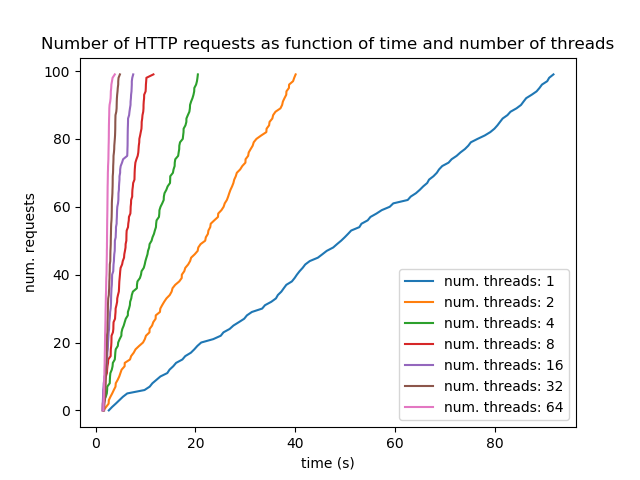
\includegraphics[width=9cm]{./Figures/results/dms_factory.png}
  \caption{Required time to perform 100 HTTP requests to a third-party API, as a function of the number of concurrent requests.}
  \label{fig:dms_factory}  
\end{figure}

Given a serial approach, which corresponds to the case in which there is only one worker thread, the system requires approximately 100 seconds to perform all queries. Thus, the time for the remote API server to respond to one query is, on average, one second. It is possible to increase the number of requests per second, by opting for a concurrent approach. Figure \ref{fig:dms_factory} shows that by performing two concurrent requests, the response time drops to half. As the number of concurrent requests increases, the response time decreases. 

However, this decrease is not always linear. While the first concurrent requests have a very positive effect in the reduction of the response time, this behavior eventually reaches a stagnation point, in which continuing to increase the number of concurrent requests has a negative effect. Thus, it is recommended to be sensible upon defining the number of concurrent requests. Despite this, the proposed DMS allows the collection of 100 requests in less than 5 seconds, which is over 20 times faster than the serial approach.

After collecting the necessary set of flights, the proposed system determines the response to a request by running the appropriate optimization algorithms. Each request is solved using the nearest neighbour heuristic, and the SA and ACO metaheuristics. For each request, it is necessary to run the optimization algorithms for a total of three times, one for each objective function (price, flight duration and entropy). While the nearest neighbour runs until a solution is found, it is possible to define multiple stop criteria for the metaheuristics, as it was referred in section \ref{sec:os_eval}. In this particular evaluation, it was defined that each optimization algorithm may run for a maximum of 1 second, or 10.000 iterations.

As a result, the total time that is necessary to respond to a request, as a function of the number of nodes and length of the start period, is illustrated in figure \ref{fig:response_time}. The analysis of this figure shows that requests with up to 10 nodes are solved in less than 60 seconds. It also shows that the response time increases non-linearly as the number of nodes increases. On the other hand, increasing the length of the start interval has low influence for small instances (up to 10 nodes), but has a significant impact for greater instances.

\begin{figure}
  \centering
  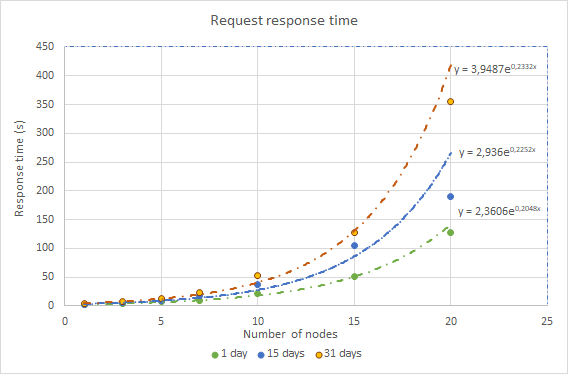
\includegraphics[width=9cm]{./imgs/response_time.png}
  \caption{Total response time to a request, as a function of the number of nodes and length of start period.}
  \label{fig:response_time}  
\end{figure}


% Note that the nearest neighbor and metaheuristics run only after the complete weight matrix is available, which occurs only once the communication with the third-party API is finished. Note also that, after the weight matrix is complete, the nearest neighbor is run first, followed by the metaheuristic for the cost, and finally by the metaheuristic for the entropy. Thus, the completion time of the nearest neighbor, gives a good estimation, or "upper bound", on the time spent communicating with the third-party API, as to obtain the necessary flight data. Figure \ref{fig:kiwi_response_time} presents an accurate illustration of the time spent communicating with the third-party API, as a function of the number of nodes, and the length of the start-period.  



% As to simplify the comprehension of the results presented in table \ref{tab:utility_0}, figure \ref{fig:prices_0} illustrates the improvement of the total flight cost, for the NN and metaheuristic algorithms, relative to the cost of the initial \textit{random} solution. It is worth noting that, for a single node (round flight), the initial random solution, the nearest neighbor, and the metaheuristic, all produce the same result. For 3 nodes, the nearest neighbor does not present relevant improvement, while the metaheuristic already distances itself, presenting around 5\% improvement. For 5 nodes, this difference increases to 20\%, and at 10 nodes it reaches the 50\% mark. Instances with more nodes, 15-20, continue to improve, slowly, up to 60\%.





% We also analyzed the impact of using different objective functions in the optimization process. Instead of optimizing for the total trip cost, the algorithm was set to minimize the entropy, that is, the weighted summation of the flight cost and flight duration. The entropy is set such that the cost weight contributes with 70\%, and the flight duration with the remaining 30\%. After executing the metaheuristic for both objective functions, the total flight cost and duration are compared. The results are illustrated in figure \ref{fig:cost_vs_time}. The inspection of this figure leads to the conclusion that, in general, by increasing the cost by around 20\%, the flight duration decreases to approximately half.


% This series of experiments is completed with the execution of the same problems, this time with a start-period of 31 days. The impact in the solution improvement, relative to the trip cost, can be verified in figure \ref{fig:prices_31}. The analysis of this figure leads to the conclusion that, the selection of an extended start-period, as opposed to a single date, leads to a higher increase in the total savings. For the round flight, the improvement of the metaheuristic is around 10\%. This is because the random and the nearest neighbor solution consider a single start date for the solution construction process. Other small instances, with 3 and 5 nodes, present much higher improvements than those with a single start date, ranging from 20-40\%, as opposed to just 5-20\%. For bigger problem instances, the effect of increasing the start-period is less significant, but it exists, providing an improvement of up to 65\%.






\section{Comparison with \textit{Kiwi}'s \textit{Nomad}}
\label{sec:nomad}

At the present time, \textit{Kiwi}'s \textit{Nomad} is the only (non-disclosed) tool that is capable of addressing the formalized \textit{Flying Tourist Problem} in the form of an unconstrained multi-city routing problem, although limited to only 10 different nodes. To facilitate the comparison of the conceived optimization system with this tool, the definition of the user requests of the proposed FTP (see section \ref{sec:ftp}) was kept as similar as possible to \textit{Kiwi}'s \textit{Nomad} interface. The user is asked to specify the departing/arriving city, together with the start date, the set of cities to be visited and the duration of the stay in each city.

The results provided by both applications were directly compared against each other, according to each considered objective function. The difference in the total flight price and duration (for each query) was also measured and analyzed as a function of the query parameters. The former evaluation will be called \textit{absolute comparison} (subsection \ref{sec:absolute_eval}), while the latter \textit{quantitative evaluation} (subsection \ref{sec:quantitative_eval}).

The execution of these tests involved over 100 different queries, by varying not only the number of nodes (2-10), but also the length of the trip start interval (1-15 days). All queries that were performed on both applications had its start and return city set to Lisbon (Portugal), while each city to be visited belongs to the same set of hub airports that were considered in the previous subsections.  These queries were executed during the period between 15 and 16 of June 2018 and the base start date was set to the 1st of August 2018, which, at the time of the tests, was 45 days in the future. The staying period in each city was set to a random value between 1 and 5 days. For extended start periods, the base start date was extended by 31 days.


\subsection{Absolute comparison}
\label{sec:absolute_eval}

Both applications respond to each query with three different sets of flights, serving the following different optimization criteria: the \textit{cheapest}, the \textit{fastest} and the \textit{recommended}. For each query, a winner was determined according to the following criteria. The cheapest set of flights is determined according to the total flight price, while the fastest depends solely on the total flight duration. The recommended set of flights depends on both the price and the duration, and the winner for this criteria must have both lower prices and duration. 

\begin{figure}[h]
    \centering
    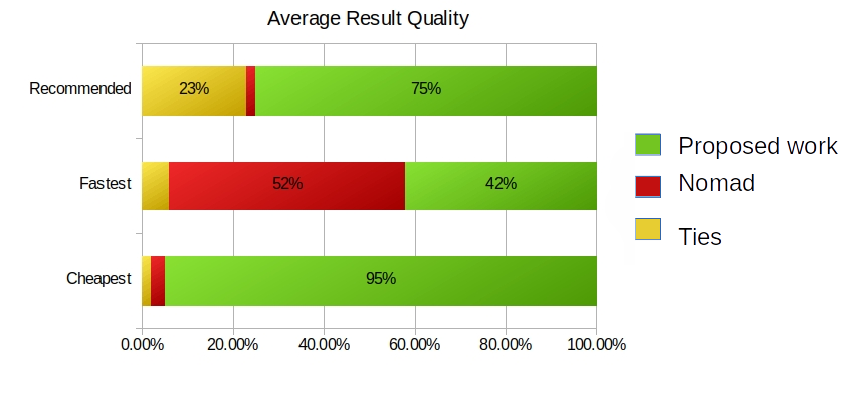
\includegraphics[width=8.5cm]{./imgs/results.png}
    \caption{Comparison of the results provided by the proposed tool and by \textit{Kiwi}'s \textit{Nomad} application.}
    \label{fig:quality_apis}
\end{figure}

Fig.~\ref{fig:quality_apis} illustrates the obtained comparison, by presenting the total number of times that an application outperformed the other, for each of the three different optimization criteria. It also shows the number of cases in which the responses were very similar.

The analysis of this figure indicates that the developed application presents better solutions for a significant amount of queries. In fact, while the fastest set of flights is only achieved in 42\% of the queries, it presents the cheapest set of flights 95\% of the times and the best recommended result 75\% of the times. 

The developed application presents high quality results for two of the three objective functions, in a consistent way. However, it does not perform particularly well in the minimization of the total flight duration. This occurs because of an implementation detail in the DMS. Upon receiving a list of flights for a query, the DMS selects only a subset of these flights, as to reduce the required amount of memory. This subset always selects the cheapest set of flights. However, in general, if a flight is fast, its price is high. Thus, upon selecting the subset of flights, the most promising solution components for the minimization of the total flight duration are discarded.


%The analysis of this figure indicates that the developed application presents better solutions for a significant amount of queries. In fact, is presents the cheapest set of flights in 95\% of the queries, and the best recommended results 75\% of the time.





\subsection{Quantitative evaluation}
\label{sec:quantitative_eval}

To evaluate the difference of the responses provided by both applications, the total flight price and duration of the recommended set of flights was also quantitatively measured (see Fig.~\ref{fig:comparison}). The values presented in these graphs refer to the developed application response and were normalized using the \textit{Kiwi}'s \textit{Nomad} response as reference. 

% \begin{figure}[!tbp]
%   \centering
%   \begin{minipage}[b]{0.4\textwidth}
%     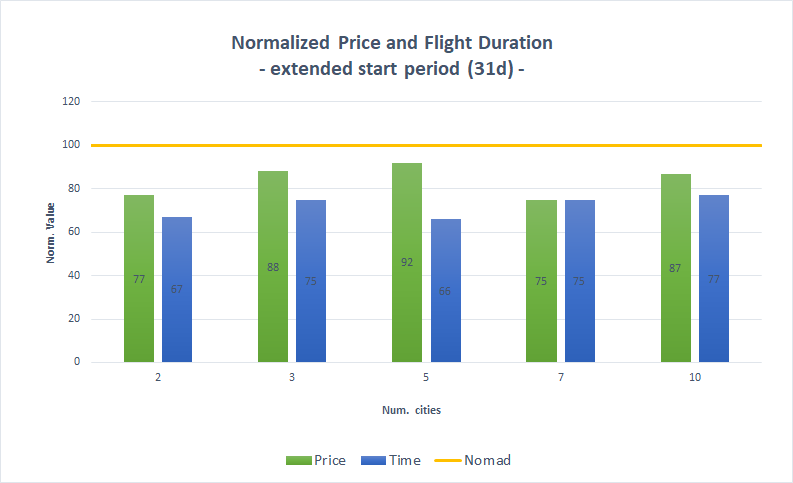
\includegraphics[width=\textwidth]{./imgs/normalized_results_es.png}
%     \caption{Flower one.}
%   \end{minipage}
%   \hfill
%   \begin{minipage}[b]{0.4\textwidth}
%     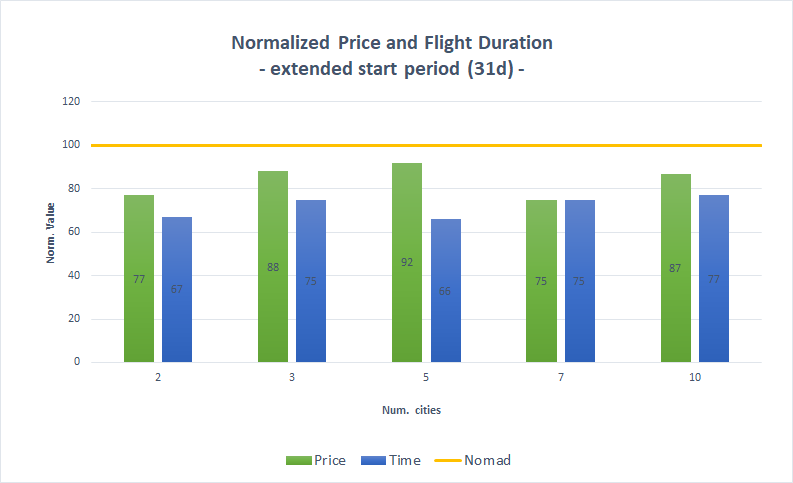
\includegraphics[width=\textwidth]{./imgs/normalized_results_es.png}
%     \caption{Flower two.}
%   \end{minipage}
% \end{figure}

%\todo{E preferivel ter esta imagem lado a lado ou uma em cima da outra}

\begin{figure}[h]
\centering
  \begin{subfigure}{0.49\linewidth} \centering
     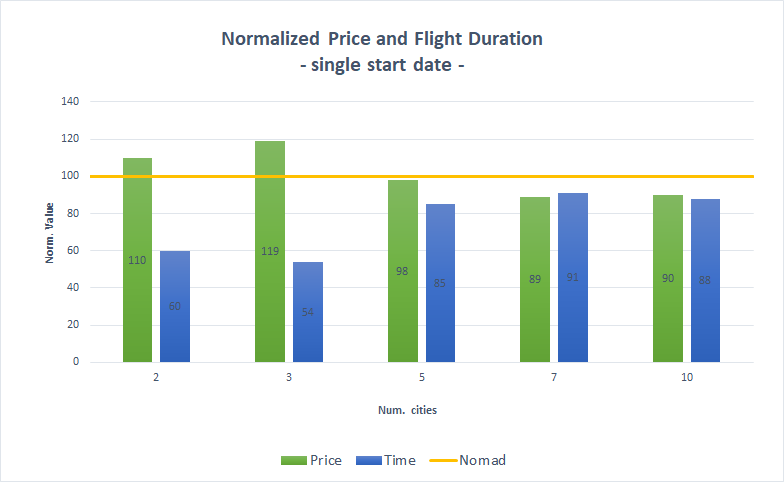
\includegraphics[scale=0.4]{./imgs/normalized_results_ss.png}
     \caption{Single start date.}\label{fig:comparison_a}
  \end{subfigure}
  \begin{subfigure}{0.49\linewidth} \centering
     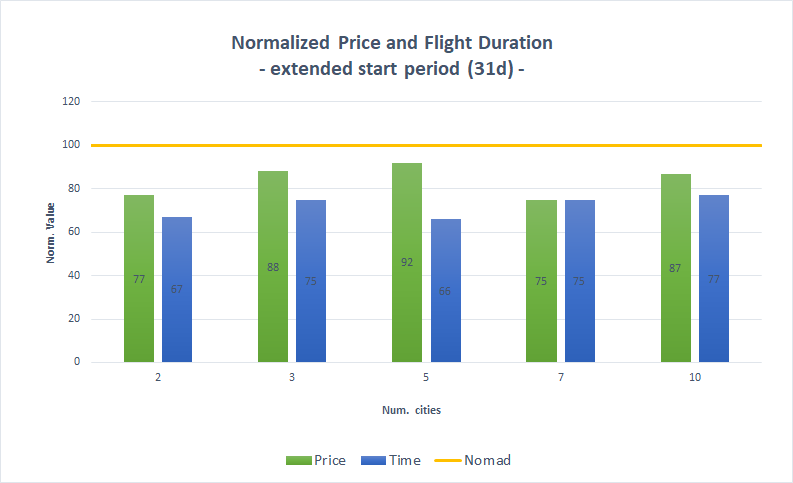
\includegraphics[scale=0.4]{./imgs/normalized_results_es.png}
     \caption{Extended start period (31 days)}\label{fig:comparison_b}
  \end{subfigure}
\caption{Comparison of the recommended flights price and duration, as a function of the number of nodes and the length of start interval. The presented values refer to the proposed application response, and were normalized with respect to \textit{Kiwi}'s \textit{Nomad} response value.}
\label{fig:comparison}
\end{figure}

Figure \ref{fig:comparison_a} presents the results of the queries performed for a single start date. Its analysis shows that, for a small number of nodes (2 and 3), the developed application recommends flights that are slightly more expensive ($\approx$ 10\% to 19\%) but have a much lower flight duration ($\approx$ 33\%-46\%). For requests with more nodes (5 to 10), the results presented by the developed application have both lower prices ($\approx$ 2\%-18\%) and flight duration ($\approx$ 9\%-24\%).

Figure \ref{fig:comparison_b} depicts the obtained results when the length of the start interval was extended to 31 days. With such an extended start period, every recommended set of flights provided by the proposed application has a lower price and duration. The price presents the most significant change: the minimum improvement is 8\%, while the maximum is 29\%.

Finally, it is worth noting that all the presented experiments only consider up to 10 different cities to be visited by the traveler. The reason why more nodes were not considered arises not from the developed application (which could easily accommodate more cities), but is motivated by a strict limit presented by \textit{Kiwi}'s \textit{Nomad} application, which does not support more than 10 nodes in the planned route.
  

% \subsubsection{Evaluating optimization performance}
% Given the more than 100 different queries considered, we compared the quality of the responses of both application for each optimization criteria. The results are presented in figure \ref{fig:quality_apis},
% and show that Bfly consistently present higher quality results, for both the cheapest, and the recommended set of flights. \textbf{Out of 100 different queries, Bfly presented the cheapest set of flights 95 times}, loosing three times to Kiwi, and tying two. As for the recommended set of flights, Bfly presents the better response 75 times, looses twice, and presents similar responses to Kiwi's 23 times. 

% \begin{figure}
%     \centering
%     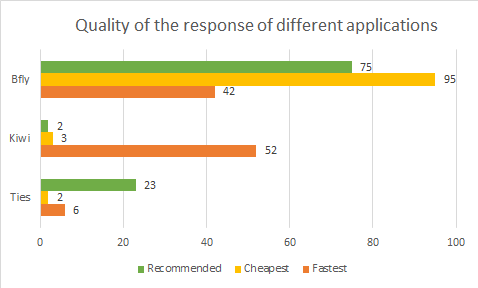
\includegraphics[width=8.5cm]{./imgs/quality_apis.png}
%     \caption{Comparison of the quality of the results of Bfly API, and Kiwi's \textit{Nomad} application.}
%     \label{fig:quality_apis}
% \end{figure}

% % We also analyzed the average quality improvement of Bfly compared to Kiwi's Nomad. These results are presented in table \ref{tab:kiwi_vs_bfly_1} and \ref{tab:kiwi_vs_bfly_15} for a single start date, and for a range of start dates (15 days), respectively. In both cases, Bfly consistently presents better results. For the extended start period, Kiwi wins only in 4 different occasions (2,5,8 and 9 nodes), and only for one optimization criteria (fastest trip). For the single start date, both applications present high quality responses for 2, 3 and 4 nodes. In these cases, one application presents better results for one criteria, but looses or ties in the other two criteria. As the number of nodes increases (5 to 10), Bfly reports better results for the cheapest and recommended set of flights.

% % \begin{figure}[h!]
% %     \centering
% %     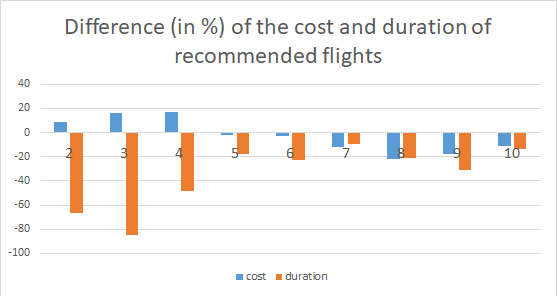
\includegraphics[width=8.5cm]{./imgs/recommended_1.png}
% %     \caption{Difference in flight cost and duration, for a single start date, as a function of the number of nodes.}
% %     \label{fig:quality_apis}
% % \end{figure}

% % \begin{figure}[h!]
% %     \centering
% %     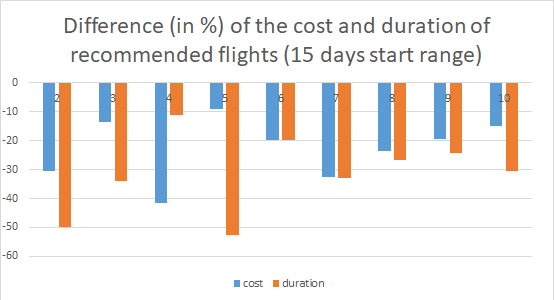
\includegraphics[width=8.5cm]{./imgs/recommended_15.png}
% %     \caption{Comparison of difference in flight cost and duration, for a range of start dates (15 days), as a function of the number of nodes.}
% %     \label{fig:quality_apis}
% % \end{figure}


% \begin{figure}
% \centering
% \begin{subfigure}[a]{0.5\textwidth}
%   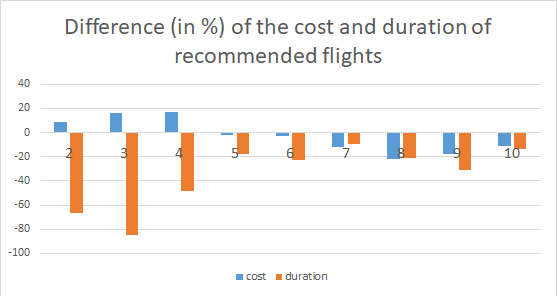
\includegraphics[width=1\linewidth]{./imgs/recommended_1.png}
%   \caption{}
%   \label{fig:Ng1} 
% \end{subfigure}

% \begin{subfigure}[b]{0.5\textwidth}
%   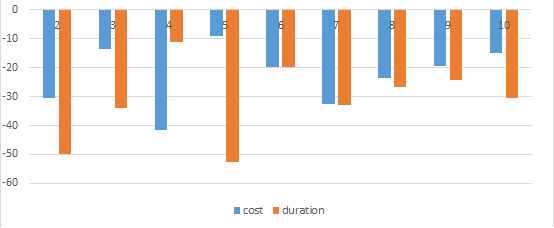
\includegraphics[width=1\linewidth]{./imgs/recommended_15_clean.png}
%   \caption{}
%   \label{fig:Ng2}
% \end{subfigure}

% \caption[asadadsa]{Difference, in \%, of the total cost and flight duration of the recommended set of flights, as a function of number of nodes. A negative value indicates that Bfly presents a lower value response, and thus, a positive result. (a) indicates queries with a single start date. (b) indicates queries with an extended start period (15 days).}
% \label{fig:recommended}
% \end{figure}

% Figure \ref{fig:recommended} enables the comparison of the total flight prices and duration between the responses of Kiwi and Bfly applications. The presented values are relative to that presented by Kiwi. Thus, a negative value in the price/duration indicates that Bfly presented a lower value response, and thus, a better result. This figure is also divided into two subplots, one for a single start date (a), and another for an extended start period (b). 

% From the analysis of figure \ref{fig:Ng1}, it can be seen that, for a low number of nodes (2, 3 and 4),
% Kiwi presents flights which are cheaper ($\approx$ 10-20\%), but slower ($\approx$ 40-80\%). However, for 5 to 10 nodes, Bfly presents results of higher quality. For 5 and 6 nodes, the cost improvement is not relevant ($\approx$ 2-3\%), but there is a considerable improvement in the flight duration ($\approx$ 20\%). As the number of nodes increases, so does the cost improvement ($\approx$ 10-20\%).

% In its turn, figure \ref{fig:Ng2} indicates that the overall quality of Bfly results improve for queries with an extended start period. First of all, Bfly always presents the better result, compared to Kiwi: for any number of nodes, the total flight duration and cost is lower. Furthermore, the cost improvement is considerably higher for extended start periods: the minimum improvement is $\approx$ 10\%, while the maximum is greater than 30\%. 



\cleardoublepage
%
%Chapter 8
\fancychapter{Conclusions}
\cleardoublepage
\label{cap:cc}
Placeholder for the conclusions.
\cleardoublepage




%
% -----------------------------------------------------------------------------




















% BIBLIOGRAPHY
% Add the Bibliography to the PDF table of contents (not the document table of contents)
\pdfbookmark[0]{Bibliography}{bib}
% The bibliography style sheet
% Chose your preferences on the format of the entries and the Labels:
% IEEEtran: Used in general (recommended for IST Thesis)
%           Entries are labelled and sorted by appearance in the document
%           Labels are Numeric inside square brackets
\bibliographystyle{IEEEtran}
%
% Apalike:  Entries formatted alphabetically, last name first, with identation
%           Labels with Autor's Name and Year inside square brackets
%\bibliographystyle{apalike}
%
% Alpha:    Entries formatted with Autor's Name and Year, hanging identation
%           Labels with Autor's abbr. Names and Year inside square brackets
%\bibliographystyle{alpha}
%
% Acm:     Entries formatted with Autor's Name (small Caps), hanging identation
%          Labels are Numeric inside square brackets
%\bibliographystyle{acm}
% The following command resets the 'emphasis' style for bibliography entries
\normalem
% Name of your BiBTeX file
\bibliography{./Thesis-MSc-Bibliography} % Put here your own filename
%
% The following command modifies the 'emphasis' style for bibliography entries
\ULforem
% If Printing on DOUBLE SIDED pages, the second page should be white.
% Otherwise, comment the following command:
\cleardoublepage
%
% -----------------------------------------------------------------------------
% HERE GO THE APPENDIXES IF REQUIRED
% If not required just comment the blocks
\appendix
%% First Appendix
\pdfbookmark[1]{Appendix A}{appendix}
% #############################################################################
% This is Appendix A
% !TEX root = ../main.tex
% #############################################################################
\chapter{Code of Project}
\label{chapter:appendixA}

Nulla dui purus, eleifend vel, consequat non, dictum porta, nulla. Duis ante mi, laoreet ut, commodo eleifend, cursus nec, lorem. Aenean eu est. Etiam imperdiet turpis. Praesent nec augue. Curabitur ligula quam, rutrum id, tempor sed, consequat ac, dui. Vestibulum accumsan eros nec magna. Vestibulum vitae dui. Vestibulum nec ligula et lorem consequat ullamcorper. 

\begin{lstlisting}[frame=lines,style=XML,caption={Example of a XML file.},label=xmlEx]
<?xml version="1.0" encoding="UTF-8"?>
<StreamInfo version="2.0">
    <Clip duration="PT01M0.00S">
        <BaseURL>videos/</BaseURL>
        <Description>svc_1</Description>
        <Representation mimeType="video/SVC" codecs="svc" frameRate="30.00" bandwidth="401.90"
            width="176" height="144" id="L0">
            <BaseURL>svc_1/</BaseURL>
            <SegmentInfo from="0" to="11" duration="PT5.00S">
                <BaseURL>svc_1-L0-</BaseURL>
            </SegmentInfo>
        </Representation>
        <Representation mimeType="video/SVC" codecs="svc" frameRate="30.00" bandwidth="1322.60"
            width="352" height="288" id="L1">
            <BaseURL>svc_1/</BaseURL>
            <SegmentInfo from="0" to="11" duration="PT5.00S">
                <BaseURL>svc_1-L1-</BaseURL>
            </SegmentInfo>
        </Representation>
    </Clip>
</StreamInfo>
\end{lstlisting}

Etiam imperdiet turpis. Praesent nec augue. Curabitur ligula quam, rutrum id, tempor sed, consequat ac, dui. Maecenas tincidunt velit quis orci. Sed in dui. Nullam ut mauris eu mi mollis luctus. Class aptent taciti sociosqu ad litora torquent per conubia nostra, per inceptos hymenaeos. Sed cursus cursus velit. Sed a massa. Duis dignissim euismod quam.

\begin{spacing}{0.5}
\lstinputlisting[style=coloredASM,language=Assembler,numbers=left,caption={Assembler Main Code.},label=code]
{./tables_and_code/example.asm.txt}
\end{spacing}


Class aptent taciti sociosqu ad litora torquent per conubia nostra, per inceptos hymenaeos. Phasellus eget nisl ut elit porta ullamcorper. Maecenas tincidunt velit quis orci. Sed in dui. Nullam ut mauris eu mi mollis luctus. Class aptent taciti sociosqu ad litora torquent per conubia nostra, per inceptos hymenaeos.

This inline MATLAB code \mcode{for i=1:3, disp('cool'); end;} uses the \verb|\mcode{}| command.\footnote{MATLAB Works also in footnotes: \mcodefn{for i=1:3, disp('cool'); end;}}

Nullam ut mauris eu mi mollis luctus. Class aptent taciti sociosqu ad litora torquent per conubia nostra, per inceptos hymenaeos. Sed cursus cursus velit. Sed a massa. Duis dignissim euismod quam. Nullam euismod metus ut orci.

\begin{lstlisting}[language=matlabfloz,caption={\mcode{Matlab Function}}]
for i = 1:3
	if i >= 5 && a ~= b       % literate programming replacement
		disp('cool');         % comment with some §\mcommentfont\LaTeX in it: $\mcommentfont\pi x^2$§
	end
	[:,ind] = max(vec);
	x_last = x(1,end) - 1;
	v(end);
	ylabel('Voltage (µV)');
end
\end{lstlisting}

Nullam ut mauris eu mi mollis luctus. Class aptent taciti sociosqu ad litora torquent per conubia nostra, per inceptos hymenaeos. Sed cursus cursus velit. Sed a massa. Duis dignissim euismod quam. Nullam euismod metus ut orci.

\lstinputlisting[
	label=lst:matlab_code,
	caption={\mcode{function.m}},
	breaklines=true
	]{./tables_and_code/function.m}

Class aptent taciti sociosqu ad litora torquent per conubia nostra, per inceptos hymenaeos. Phasellus eget nisl ut elit porta ullamcorper. Maecenas tincidunt velit quis orci. Sed in dui. Nullam ut mauris eu mi mollis luctus. Class aptent taciti sociosqu ad litora torquent per conubia nostra, per inceptos hymenaeos. Sed cursus cursus velit. Sed a massa. Duis dignissim euismod quam. Nullam euismod metus ut orci. Vestibulum erat libero, scelerisque et, porttitor et, varius a, leo.

\begin{lstlisting}[style=htmlcssjs,caption={HTML with CSS Code}]
<!DOCTYPE html>
<html>
  <head>
    <title>Listings Style Test</title>
    <meta charset="UTF-8">
    <style>
      /* CSS Test */
      * {
        padding: 0;
        border: 0;
        margin: 0;
      }
    </style>
    <link rel="stylesheet" href="css/style.css" />
  </head>
  <header> hey </header>
  <article> this is a article </article>
  <body>
    <!-- Paragraphs are fine -->
    <div id="box">			
			<p>
			  Hello World
			</p>
      <p>Hello World</p>
      <p id="test">Hello World</p>
			<p></p>
    </div>
    <div>Test</div>
    <!-- HTML script is not consistent -->
    <script src="js/benchmark.js"></script>
    <script>
      function createSquare(x, y) {
        // This is a comment.
        var square = document.createElement('div');
        square.style.width = square.style.height = '50px';
        square.style.backgroundColor = 'blue';
        
        /*
         * This is another comment.
         */
        square.style.position = 'absolute';
        square.style.left = x + 'px'; 
        square.style.top = y + 'px';
        
        var body = document.getElementsByTagName('body')[0];
        body.appendChild(square);
      };
      
      // Please take a look at +=
      window.addEventListener('mousedown', function(event) {
        // German umlaut test: Berührungspunkt ermitteln
        var x = event.touches[0].pageX;
        var y = event.touches[0].pageY;
        var lookAtThis += 1;
      });
    </script>
  </body>
</html>
\end{lstlisting}

Nulla dui purus, eleifend vel, consequat non, dictum porta, nulla. Duis ante mi, laoreet ut, commodo eleifend, cursus nec, lorem. Aenean eu est. Etiam imperdiet turpis. Praesent nec augue. Curabitur ligula quam, rutrum id, tempor sed, consequat ac, dui. Vestibulum accumsan eros nec magna. Vestibulum vitae dui. Vestibulum nec ligula et lorem consequat ullamcorper.

\begin{lstlisting}[style=htmlcssjs,caption={HTML CSS Javascript Code}]

@media only screen and (min-width: 768px) and (max-width: 991px) {
	
	#main {
		width: 712px;
		padding: 100px 28px 120px;
	}
	
	/* .mono {
		font-size: 90%;
	} */
	
	.cssbtn a {
		margin-top: 10px;
		margin-bottom: 10px;
		width: 60px;  
		height: 60px;   
		font-size: 28px;
		line-height: 62px;
	}
\end{lstlisting}

Nulla dui purus, eleifend vel, consequat non, dictum porta, nulla. Duis ante mi, laoreet ut, commodo eleifend, cursus nec, lorem. Aenean eu est. Etiam imperdiet turpis. Praesent nec augue. Curabitur ligula quam, rutrum id, tempor sed, consequat ac, dui. Vestibulum accumsan eros nec magna. Vestibulum vitae dui. Vestibulum nec ligula et lorem consequat ullamcorper.

\begin{lstlisting} [style=py,caption={PYTHON Code}]
class TelgramRequestHandler(object):
    def handle(self):
        addr = self.client_address[0]         # Client IP-adress
        telgram = self.request.recv(1024)     # Recieve telgram
        print "From: %s, Received: %s" % (addr, telgram)
        return
\end{lstlisting}
%% If Printing on DOUBLE SIDED pages, the second page should be white.
%% Otherwise, comment the following command:
\cleardoublepage
%% Second Appendix
\pdfbookmark[1]{Appendix B}{appendix}
% #############################################################################
% This is Appendix B
% !TEX root = ../main.tex
% #############################################################################
\chapter{A Large Table}
\label{chapter:appendixB}

Aliquam et nisl vel ligula consectetuer suscipit. Morbi euismod enim eget neque. Donec sagittis massa. Vestibulum quis augue sit amet ipsum laoreet pretium. Nulla facilisi. Duis tincidunt, felis et luctus placerat, ipsum libero vestibulum sem, vitae elementum wisi ipsum a metus. Nulla a enim sed dui hendrerit lobortis. Donec lacinia vulputate magna. Vivamus suscipit lectus at quam. In lectus est, viverra a, ultricies ut, pulvinar vitae, tellus. Donec et lectus et sem rutrum sodales. Morbi cursus. Aliquam a odio. Sed tortor velit, convallis eget, porta interdum, convallis sed, tortor. Phasellus ac libero a lorem auctor mattis. Lorem ipsum dolor sit amet, consectetuer adipiscing elit.

Nunc auctor bibendum eros. Maecenas porta accumsan mauris. Etiam enim enim, elementum sed, bibendum quis, rhoncus non, metus. Fusce neque dolor, adipiscing sed, consectetuer et, lacinia sit amet, quam. Suspendisse wisi quam, consectetuer in, blandit sed, suscipit eu, eros. Etiam ligula enim, tempor ut, blandit nec, mollis eu, lectus. Nam cursus. Vivamus iaculis. Aenean risus purus, pharetra in, blandit quis, gravida a, turpis. Donec nisl. Aenean eget mi. Fusce mattis est id diam. Phasellus faucibus interdum sapien. Duis quis nunc. Sed enim.
Nunc auctor bibendum eros. Maecenas porta accumsan mauris. Etiam enim enim, elementum sed, bibendum quis, rhoncus non, metus. Fusce neque dolor, adipiscing sed, consectetuer et, lacinia sit amet, quam.

% Table Example
\newcommand{\greyrow}{\rowcolor[rgb]{0.9,0.9,0.9}}
\newcommand{\whiterow}{\rowcolor[rgb]{1,1,1}}
\newcommand{\greycell}[1]{\multicolumn{1}{{>{\columncolor[rgb]{0.9,0.9,0.9}}c}}{#1}}
\newcommand{\lightgreycell}[1]{\multicolumn{1}{{>{\columncolor[rgb]{0.9,0.9,0.9}}c}}{#1}}
\newcommand{\mediumgreycell}[1]{\multicolumn{1}{{>{\columncolor[rgb]{0.8,0.8,0.8}}c}}{#1}}
\newcommand{\darkgreycell}[1]{\multicolumn{1}{{>{\columncolor[rgb]{0.7,0.7,0.7}}c}}{#1}}
\newcommand{\whitecell}[1]{\multicolumn{1}{{>{\columncolor[rgb]{1,1,1}}c}}{#1}}

\newcommand{\cellformatG}[1]{\multicolumn{1}{{>{\columncolor[rgb]{.9,.9,.9}}c}}{#1}}
\newcommand{\cellformatW}[1]{\multicolumn{1}{{>{\columncolor[rgb]{1,1,1}}c}}{#1}}
\newcommand{\cellformatlG}[1]{\multicolumn{1}{{|>{\columncolor[rgb]{.9,.9,.9}}c}}{#1}}
\newcommand{\cellformatlW}[1]{\multicolumn{1}{{|>{\columncolor[rgb]{1,1,1}}c}}{#1}}
\newcommand{\cellformatrG}[1]{\multicolumn{1}{{>{\columncolor[rgb]{.9,.9,.9}}c|}}{#1}}
\newcommand{\cellformatrW}[1]{\multicolumn{1}{{>{\columncolor[rgb]{1,1,1}}c|}}{#1}}
\newcommand{\cellformatlrG}[1]{\multicolumn{1}{{|>{\columncolor[rgb]{.9,.9,.9}}c|}}{#1}}
\newcommand{\cellformatlrW}[1]{\multicolumn{1}{{|>{\columncolor[rgb]{1,1,1}}c|}}{#1}}

\begin{table}[t]
\centering
\caption{Example table}
\label{table:table1}
\begin{tabular}{c c c c c c}
\hline
\cellformatrG{}&\cellformatlG{}&\cellformatrG{}&\cellformatlG{}&\cellformatrG{}&\cellformatlG{}\\
\cellformatrG{}&
\cellformatlG{\multirow{-2}{*}{\centering\bf \#Layers}} & 
\cellformatrG{\multirow{-2}{*}{\centering\bf \#Nets}} & 
\cellformatlG{\multirow{-2}{*}{\centering \#Nodes\Mark1}} & 
\cellformatrG{\multirow{-2}{1.8cm}{\centering Critical path}}&
\cellformatlG{\multirow{-2}{2cm}{\centering\bf Latency ($T_{iter}$)}}\\
\cellformatrG{\multirow{-3}{2.2cm}{\centering Benchmark: ANN}} &
\cellformatlG{\footnotesize $(1)$} & 
\cellformatrG{\footnotesize$(2)$} & 
\cellformatlG{\footnotesize$(3)=8\cdot(1)\cdot(2)$} & 
\cellformatrG{\footnotesize$(4)=4\cdot(1)$} & 
\cellformatlG{\footnotesize$(5)$}\\
\hline
\cellformatrW{A1} & \cellformatlW{\bf 3--1501} & \cellformatrW{       1   } & \cellformatlW{\bf 24--12008}  & \cellformatrW{\bf 12--6004} & \cellformatlW{    4}\\
\cellformatrW{A2} & \cellformatlW{    501    } & \cellformatrW{       1   } & \cellformatlW{     4008    }  & \cellformatrW{  2004      } & \cellformatlW{\bf 2--2000 }\\
\cellformatrW{A3} & \cellformatlW{     10    } & \cellformatrW{\bf 2--1024} & \cellformatlW{\bf 160--81920} & \cellformatrW{    40      } & \cellformatlW{   60\Mark2 }\\
\cellformatrW{A4} & \cellformatlW{     10    } & \cellformatrW{      50   } & \cellformatlW{     4000    }  & \cellformatrW{    40      } & \cellformatlW{\bf 80--1200}\\
\hline
\multicolumn{6}{c}{\vspace*{-0.3cm}}\\
%%%%%%%%%%%%% SECOND PART OF THE TABLE %%%%%%%%%%%%%%%%%%%%%%%%
\hline
\cellformatrG{}&\cellformatlG{}&\cellformatrG{}&\cellformatlG{}&\cellformatrG{}&\cellformatlG{}\\
\cellformatrG{}&
\cellformatlG{\multirow{-2}{1.6cm}{\centering\bf FFT size\Mark3}} & 
\cellformatrG{\multirow{-2}{*}{\centering\it\#Inputs}} & 
\cellformatlG{\multirow{-2}{*}{\centering\it \#Nodes\Mark1}} & 
\cellformatrG{\multirow{-2}{1.8cm}{\centering\it Critical path}}&
\cellformatlG{\multirow{-2}{2cm}{\centering\bf Latency ($T_{iter}$)}}\\
\cellformatrG{\multirow{-3}{2.2cm}{\centering Benchmark: FFT}}& 
\cellformatlG{\footnotesize$(1)$} & 
\cellformatrG{\footnotesize$(2)=2^{(1)}$} & 
\cellformatlG{\footnotesize$(3)=10\cdot(1)\cdot (2)$} & 
\cellformatrG{\footnotesize$(4)=4\cdot (1)$} & 
\cellformatlG{\footnotesize$(5)$}\\
\hline
\cellformatrW{F1} & \cellformatlW{\bf 1--10} & \cellformatrW{2--1024} & \cellformatlW{\bf 20--102400} &  \cellformatrW{4--40} & \cellformatlW{6--60\Mark2}\\
\cellformatrW{F2} & \cellformatlW{\bf 5} & \cellformatrW{32} & \cellformatlW{1600} & \cellformatrW{20} & \cellformatlW{\bf 40 -- 1500}\\
\hline
\multicolumn{6}{c}{\vspace*{-0.3cm}}\\
% THIRD AND LAST TABLE!!!
\hline
\cellformatrG{}&\cellformatlG{}&\cellformatrG{}&\cellformatlG{}&\cellformatrG{}&\cellformatlG{}\\
\cellformatrG{}&
\cellformatlG{\multirow{-2}{*}{\centering\bf\#Types}} & 
\cellformatrG{\multirow{-2}{*}{\centering\bf \#Nodes}} & 
\cellformatlG{\multirow{-2}{*}{\centering\it \#Networks}} & 
\cellformatrG{\multirow{-2}{1.8cm}{\centering\it Critical path}}&
\cellformatlG{\multirow{-2}{2cm}{\centering\bf Latency ($T_{iter}$)}}\\
\cellformatrG{\multirow{-3}{2.2cm}{\centering Benchmark: Random networks}}& 
\cellformatlG{\footnotesize$(1)$} & 
\cellformatrG{\footnotesize$(2)$} & 
\cellformatlG{\footnotesize$(3)$} &
\cellformatrG{\footnotesize$(4)$} & 
\cellformatlG{\footnotesize$(5)$}\\
\hline
\cellformatrW{R1} & \cellformatlW{3} & \cellformatrW{10--2000} & \cellformatlW{500} &  \cellformatrW{\it variable} & \cellformatlW{\footnotesize$(4)$}\\
\cellformatrW{R2} & \cellformatlW{3} & \cellformatrW{  50    } & \cellformatlW{500} &  \cellformatrW{\it variable} & \cellformatlW{\footnotesize$(4)\times [1;\cdots;20]$}\\
\hline
\multicolumn{6}{c}{\vspace*{-0.3cm}}\\
\multicolumn{6}{l}{\it\Mark1 Excluding constant nodes.}\\
\multicolumn{6}{l}{\it\Mark2 Value kept proportional to the critical path: $(5)=(4)*1.5$.}\\
\multicolumn{6}{l}{\it\Mark3 A size of $x$ corresponds to a $2^x$ point FFT.}\\
\multicolumn{6}{l}{\it Values in bold indicate the parameter being varied.}
\end{tabular}
\end{table}

\textcolor{violet}{As \Cref{table:table1} shows, the data can be inserted from a file, in the case of a somehow complex structure. Notice the Table footnotes.}	

Lorem ipsum dolor sit amet, consectetuer adipiscing elit. Morbi commodo, ipsum sed pharetra gravida, orci magna rhoncus neque, id pulvinar odio lorem non turpis. Nullam sit amet enim. Suspendisse id velit vitae ligula volutpat condimentum. Aliquam erat volutpat. Sed quis velit. Nulla facilisi. Nulla libero. Vivamus pharetra posuere sapien. Nam consectetuer. Sed aliquam, nunc eget euismod ullamcorper, lectus nunc ullamcorper orci, fermentum bibendum enim nibh eget ipsum. Donec porttitor ligula eu dolor. Maecenas vitae nulla consequat libero cursus venenatis. Nam magna enim, accumsan eu, blandit sed, blandit a, eros. 

\textcolor{violet}{And now an example (\Cref{tab:lon_table}) of a table that extends to more than one page. Notice the repetition of the Caption (with indication that is continued) and of the Header, as well as the continuation text at the bottom.}

\begin{center}
\begin{longtable}{|l|l|l|}
\caption[Example of a very long table spreading in several pages]{Example of a very long table spreading in several pages} \label{tab:lon_table} \\

\hline \multicolumn{1}{|c|}{\textbf{Time (s)}} & \multicolumn{1}{c|}{\textbf{Triple chosen}} & \multicolumn{1}{c|}{\textbf{Other feasible triples}} \\ \hline 
\endfirsthead

\multicolumn{3}{c}%
{{\bfseries \tablename\ \thetable{} -- continued from previous page}} \\
\hline \multicolumn{1}{|c|}{\textbf{Time (s)}} &
\multicolumn{1}{c|}{\textbf{Triple chosen}} &
\multicolumn{1}{c|}{\textbf{Other feasible triples}} \\ \hline 
\endhead

\hline \multicolumn{3}{|r|}{{Continued on next page}} \\ \hline
\endfoot

\hline \hline
\endlastfoot
0 & (1, 11, 13725) & (1, 12, 10980), (1, 13, 8235), (2, 2, 0), (3, 1, 0) \\
2745 & (1, 12, 10980) & (1, 13, 8235), (2, 2, 0), (2, 3, 0), (3, 1, 0) \\
5490 & (1, 12, 13725) & (2, 2, 2745), (2, 3, 0), (3, 1, 0) \\
8235 & (1, 12, 16470) & (1, 13, 13725), (2, 2, 2745), (2, 3, 0), (3, 1, 0) \\
10980 & (1, 12, 16470) & (1, 13, 13725), (2, 2, 2745), (2, 3, 0), (3, 1, 0) \\
13725 & (1, 12, 16470) & (1, 13, 13725), (2, 2, 2745), (2, 3, 0), (3, 1, 0) \\
16470 & (1, 13, 16470) & (2, 2, 2745), (2, 3, 0), (3, 1, 0) \\
19215 & (1, 12, 16470) & (1, 13, 13725), (2, 2, 2745), (2, 3, 0), (3, 1, 0) \\
21960 & (1, 12, 16470) & (1, 13, 13725), (2, 2, 2745), (2, 3, 0), (3, 1, 0) \\
24705 & (1, 12, 16470) & (1, 13, 13725), (2, 2, 2745), (2, 3, 0), (3, 1, 0) \\
27450 & (1, 12, 16470) & (1, 13, 13725), (2, 2, 2745), (2, 3, 0), (3, 1, 0) \\
30195 & (2, 2, 2745) & (2, 3, 0), (3, 1, 0) \\
32940 & (1, 13, 16470) & (2, 2, 2745), (2, 3, 0), (3, 1, 0) \\
35685 & (1, 13, 13725) & (2, 2, 2745), (2, 3, 0), (3, 1, 0) \\
38430 & (1, 13, 10980) & (2, 2, 2745), (2, 3, 0), (3, 1, 0) \\
41175 & (1, 12, 13725) & (1, 13, 10980), (2, 2, 2745), (2, 3, 0), (3, 1, 0) \\
43920 & (1, 13, 10980) & (2, 2, 2745), (2, 3, 0), (3, 1, 0) \\
46665 & (2, 2, 2745) & (2, 3, 0), (3, 1, 0) \\
49410 & (2, 2, 2745) & (2, 3, 0), (3, 1, 0) \\
52155 & (1, 12, 16470) & (1, 13, 13725), (2, 2, 2745), (2, 3, 0), (3, 1, 0) \\
54900 & (1, 13, 13725) & (2, 2, 2745), (2, 3, 0), (3, 1, 0) \\
57645 & (1, 13, 13725) & (2, 2, 2745), (2, 3, 0), (3, 1, 0) \\
60390 & (1, 12, 13725) & (2, 2, 2745), (2, 3, 0), (3, 1, 0) \\
63135 & (1, 13, 16470) & (2, 2, 2745), (2, 3, 0), (3, 1, 0) \\
65880 & (1, 13, 16470) & (2, 2, 2745), (2, 3, 0), (3, 1, 0) \\
68625 & (2, 2, 2745) & (2, 3, 0), (3, 1, 0) \\
71370 & (1, 13, 13725) & (2, 2, 2745), (2, 3, 0), (3, 1, 0) \\
74115 & (1, 12, 13725) & (2, 2, 2745), (2, 3, 0), (3, 1, 0) \\
76860 & (1, 13, 13725) & (2, 2, 2745), (2, 3, 0), (3, 1, 0) \\
79605 & (1, 13, 13725) & (2, 2, 2745), (2, 3, 0), (3, 1, 0) \\
82350 & (1, 12, 13725) & (2, 2, 2745), (2, 3, 0), (3, 1, 0) \\
85095 & (1, 12, 13725) & (1, 13, 10980), (2, 2, 2745), (2, 3, 0), (3, 1, 0) \\
87840 & (1, 13, 16470) & (2, 2, 2745), (2, 3, 0), (3, 1, 0) \\
90585 & (1, 13, 16470) & (2, 2, 2745), (2, 3, 0), (3, 1, 0) \\
93330 & (1, 13, 13725) & (2, 2, 2745), (2, 3, 0), (3, 1, 0) \\
96075 & (1, 13, 16470) & (2, 2, 2745), (2, 3, 0), (3, 1, 0) \\
98820 & (1, 13, 16470) & (2, 2, 2745), (2, 3, 0), (3, 1, 0) \\
101565 & (1, 13, 13725) & (2, 2, 2745), (2, 3, 0), (3, 1, 0) \\
104310 & (1, 13, 16470) & (2, 2, 2745), (2, 3, 0), (3, 1, 0) \\
107055 & (1, 13, 13725) & (2, 2, 2745), (2, 3, 0), (3, 1, 0) \\
109800 & (1, 13, 13725) & (2, 2, 2745), (2, 3, 0), (3, 1, 0) \\
112545 & (1, 12, 16470) & (1, 13, 13725), (2, 2, 2745), (2, 3, 0), (3, 1, 0) \\
115290 & (1, 13, 16470) & (2, 2, 2745), (2, 3, 0), (3, 1, 0) \\
118035 & (1, 13, 13725) & (2, 2, 2745), (2, 3, 0), (3, 1, 0) \\
120780 & (1, 13, 16470) & (2, 2, 2745), (2, 3, 0), (3, 1, 0) \\
123525 & (1, 13, 13725) & (2, 2, 2745), (2, 3, 0), (3, 1, 0) \\
126270 & (1, 12, 16470) & (1, 13, 13725), (2, 2, 2745), (2, 3, 0), (3, 1, 0) \\
129015 & (2, 2, 2745) & (2, 3, 0), (3, 1, 0) \\
131760 & (2, 2, 2745) & (2, 3, 0), (3, 1, 0) \\
134505 & (1, 13, 16470) & (2, 2, 2745), (2, 3, 0), (3, 1, 0) \\
137250 & (1, 13, 13725) & (2, 2, 2745), (2, 3, 0), (3, 1, 0) \\
139995 & (2, 2, 2745) & (2, 3, 0), (3, 1, 0) \\
142740 & (2, 2, 2745) & (2, 3, 0), (3, 1, 0) \\
145485 & (1, 12, 16470) & (1, 13, 13725), (2, 2, 2745), (2, 3, 0), (3, 1, 0) \\
148230 & (2, 2, 2745) & (2, 3, 0), (3, 1, 0) \\
150975 & (1, 13, 16470) & (2, 2, 2745), (2, 3, 0), (3, 1, 0) \\
153720 & (1, 12, 13725) & (2, 2, 2745), (2, 3, 0), (3, 1, 0) \\
156465 & (1, 13, 13725) & (2, 2, 2745), (2, 3, 0), (3, 1, 0) \\
159210 & (1, 13, 13725) & (2, 2, 2745), (2, 3, 0), (3, 1, 0) \\
161955 & (1, 13, 16470) & (2, 2, 2745), (2, 3, 0), (3, 1, 0) \\
164700 & (1, 13, 13725) & (2, 2, 2745), (2, 3, 0), (3, 1, 0) \\
\end{longtable}
\end{center}
%% If Printing on DOUBLE SIDED pages, the second page should be white.
%% Otherwise, comment the following command:
\cleardoublepage

% -----------------------------------------------------------------------------
% And this is THE END of the IST Thesis Document
\end{document}